% Author: Alfredo Sánchez Alberca (asalber@ceu.es)
% !TEX program = xelatex
%----------------------------------------------------------------------------------------
%    DOCUMENT CLASS
%----------------------------------------------------------------------------------------

\documentclass[11pt,a4paper,openright]{book}
%----------------------------------------------------------------------------------------
%	PACKAGES AND OTHER DOCUMENT CONFIGURATIONS
%----------------------------------------------------------------------------------------

% Language settings
\usepackage{polyglossia}
\setdefaultlanguage{english}

% Margins and layout
\usepackage[top=3cm, bottom=3cm, left=2.54cm, right=2.54cm]{geometry}

% Math support
\usepackage{amsmath, amssymb}
% \usepackage{mathspec}

% Font settings
\usepackage{unicode-math}
\setmainfont[Ligatures=TeX]{TeX Gyre Pagella}
\setmathfont{TG Pagella Math}
% \setmathfont[math-style=ISO, bold-style=ISO]{texgyrepagella-math.otf}

% Color
\usepackage{xcolor} % Required for specifying colors by name
\definecolor{color1}{RGB}{5,161,230}
\definecolor{color2}{RGB}{238,50,36}
\definecolor{ocre}{RGB}{243,102,25} % Define the orange color used for highlighting throughout the book
\definecolor{blueceu}{RGB}{5,161,230} % Blue color of CEU logo
\definecolor{greenceu}{RGB}{185,209,16} % Green color of CEU logo
\definecolor{redceu}{RGB}{238,50,36} % Red color of CEU logo
\definecolor{grayceu}{RGB}{111,107,83} % Gray color of CEU logo
\definecolor{coral}{rgb}{1,0.5,0.31} % Orange color for graphics
\definecolor{royalblue1}{rgb}{0.28,0.46,1} % Blue color for graphics
\definecolor{mygreen}{rgb}{0,0.8,0} % Green color for graphics
\definecolor{chaptergrey}{RGB}{5,161,230} % Blue color of CEU logo

% Line breaking
\usepackage{microtype} 
\setlength{\emergencystretch}{2em}

% Graphics
\usepackage{graphicx}
\usepackage{tikz} 
\usepackage{eso-pic} % Required for specifying an image background in the title page

% Arrays and tables
\usepackage{array}
\usepackage{multirow}
\usepackage{colortbl}
\usepackage{booktabs}
\newcommand{\tcrule}{\arrayrulecolor{color1!50!white}\toprule}
\newcommand{\mcrule}{\arrayrulecolor{color1!50!white}\midrule}
\newcommand{\bcrule}{\arrayrulecolor{color1!50!white}\bottomrule}

% Captions
\usepackage[margin=20pt, font=small, labelfont=bf, labelsep=endash]{caption}

% Floating figures
\usepackage{subfigure}

% Lists
\usepackage[shortlabels]{enumitem} % Customize lists
%\setlist{nolistsep} % Reduce spacing between bullet points and numbered lists
\setlist[description]{style=sameline,leftmargin=0cm}

% Columns
\usepackage{multicol}

% Creative common icons
\usepackage[scale=2]{ccicons}

% \makeatletter
% \let\savees@listquot\es@listquot
% \def\es@listquot{\protect\savees@listquot}
% \makeatletter

% hyperlinks
\usepackage{hyperref}
\hypersetup{
pdfauthor = {Alfredo S\'anchez Alberca},
pdftitle = {Calculus practices with Geogebra},
pdfsubject = {Calculus},
pdfkeywords = {Mathematics, Calculus, Geogebra},
pdfcreator = {XeLaTeX with hyperref package},
pdfproducer = {pdfLaTeX},
colorlinks = true,
linkcolor = red,          % color of internal links
citecolor = green,        % color of links to bibliography
filecolor = magenta,      % color of file links
urlcolor = magenta,          % color of external links
}
%\usepackage{breakurl}

% Indentation
%\setlength\parindent{0pt}

% Control of widow orphan lines
\clubpenalty=10000
\widowpenalty=10000 

%Code listing formatting
\usepackage{listings}
\lstdefinelanguage{morejava}{morekeywords={String}}
\definecolor{vollgrau}{rgb}{0.9,0.9,0.9}
\definecolor{colKeys}{rgb}{0,0,1}
\definecolor{colIdentifier}{rgb}{0,0,0}
\definecolor{colComments}{rgb}{1,0.5,0}
\definecolor{colString}{rgb}{0,0.5,0}
\definecolor{colbackground}{rgb}{0.9,0.9,1}
\lstset{%
      language=R,
      float=hbp,%
      basicstyle=\ttfamily,%
      identifierstyle=\color{colIdentifier},%
      keywordstyle=\color{colKeys},%
      stringstyle=\color{colString},%
      commentstyle=\color{colCommentsxelatex},%
%    columns=flexible,%xelatex
%    columns=fullflexible,%xelatex
      columns=fixed, %xelatex
      tabsize=1,%xelatex
      extendedchars=true,%xelatex
      showspaces=false,%xelatex
      showstringspaces=false,%xelatex
      breaklines=true,%xelatex
      breakindent=10pt,%xelatex
      backgroundcolor=\color{colbackgxelatexround},%
      breakautoindent=true,%xelatex
      captionpos=t,%
      xleftmargin=1em,%
%    xrightmargin=.5\fboxsep,%
      numbersep=1em,%
      escapechar=\#\RequirePackage[\eu@zf@math]{fontspec}[2008/08/09]
}

% Set short or lon\RequirePackage[\eu@zf@math]{fontspec}[2008/08/09]ersion desired
% \usepackage[cort\RequirePackage[\eu@zf@math]{fontspec}[2008/08/09]

%----------------------------------------------------------------------------------------
%	SECTIONS AND SUBSECTIONS
%----------------------------------------------------------------------------------------
%\titleformat*{\section}{\Huge}
%\titleformat*{\subsection}{\Large}


% Chapter and section formatting 
\usepackage[rigidchapters,explicit]{titlesec}
\setlength{\fboxsep}{5pt}
\newlength{\titulolength}
\setlength{\titulolength}{\textwidth} 
\addtolength{\titulolength}{-2\fboxsep}
\addtolength{\titulolength}{-2\fboxrule}
\titleformat{\chapter}[display]
{\bfseries\sffamily}
{\filleft \mdseries \LARGE \color{blueceu} Practice \Huge\thechapter}
{0.5ex}
{\colorbox{blueceu}{\parbox[t]{\titulolength}{\rule{0mm}{10mm}\Huge\sffamily\filleft\textcolor{white}{#1}}}}
\titleformat{\section}{\normalfont\Large\bfseries\color{blueceu}}{\arabic{section}}{1em}{#1}
\titleformat{\subsection}{\normalfont\large\bfseries\color{blueceu}}{\arabic{section}.\arabic{subsection}}{1em}{#1}
\titleformat{\subsubsection}{\normalfont\normalsize\bfseries\color{blueceu}}{\arabic{section}.\arabic{subsection}.\arabic{subsubsection}}{0.5em}{#1}
\titlespacing{\chapter}{0pt}{0pt}{30ex}
\titlespacing{\section}{0pt}{8ex}{4ex}

%----------------------------------------------------------------------------------------
%	MAIN TABLE OF CONTENTS
%----------------------------------------------------------------------------------------

% \usepackage{titletoc} % Required for manipulating the table of contents
% 
% \contentsmargin{0cm} % Removes the default margin
% % Chapter text styling
% \titlecontents{chapter}[1.25cm] % Indentation
% {\addvspace{15pt}\large\bfseries} % Spacing and font options for chapters
% {\color{gray}\contentslabel[\Large\thecontentslabel.]{1.25cm}} % Chapter number
% {}  
% {\color{gray}\bfseries\hfill\thecontentspage} % Page number
% % Section text styling
% \titlecontents{section}[1.25cm] % Indentation
% {\addvspace{5pt}\bfseries} % Spacing and font options for sections
% {\contentslabel[\thecontentslabel]{1.25cm}} % Section number
% {}
% {\hfill\color{black}\thecontentspage} % Page number
% []
% % Subsection text styling
% \titlecontents{subsection}[1.25cm] % Indentation
% {\addvspace{1pt}\small} % Spacing and font options for subsections
% {\contentslabel[\thecontentslabel]{1.25cm}} % Subsection number
% {}
% {\;\titlerule*[.5pc]{.}\;\thecontentspage} % Page number
% [] 

%----------------------------------------------------------------------------------------
%	MINI TABLE OF CONTENTS IN CHAPTER HEADS
%----------------------------------------------------------------------------------------

% % Section text styling
% \titlecontents{lsection}[0em] % Indendating
% {\footnotesize\sffamily} % Font settings
% {}
% {}
% {}
% 
% % Subsection text styling
% \titlecontents{lsubsection}[.5em] % Indentation
% {\normalfont\footnotesize\sffamily} % Font settings
% {}
% {}
% {}
 
%----------------------------------------------------------------------------------------
%	PAGE HEADERS
%----------------------------------------------------------------------------------------

% Headings and footers
\usepackage{fancyhdr}
\pagestyle{fancy}
\fancyhead{}
\renewcommand{\chaptermark}[1]{\markboth{\thechapter.\ #1}{}}
\fancyhead[LE]{\scshape Matemática Aplicada con Geogebra}
\fancyhead[RO]{\sffamily\slshape \leftmark}
\renewcommand{\headrulewidth}{0pt}
\renewcommand{\floatpagefraction}{.8}
\renewcommand{\textfraction}{.1}


% \usepackage{fancyhdr} % Required for header and footer configuration
% 
% \pagestyle{fancy}
% \renewcommand{\chaptermark}[1]{\markboth{\color{grayceu}\sffamily\normalsize\textit{#1}}{}} % Chapter text font
% % settings
% %\renewcommand{\sectionmark}[1]{\markright{\color{grayceu}\sffamily\normalsize\textit{\thesection\hspace{5pt}#1}}{}} %
% % Section text font settings
% \fancyhf{} \fancyfoot[LE,RO]{\normalsize\thepage} % Font setting for the page number in the footer
% \fancyhead[RE]{{\color{grayceu}\sffamily\normalsize\textit{Pr�cticas de Bioestad�stica con R and RKTeaching}}} % Print the nearest
% % section name on the left side of odd pages
% \fancyhead[LO]{\leftmark} % Print the current chapter name on the right side of even pages
% \renewcommand{\headrulewidth}{0pt} % Removes the rule in the header
% \addtolength{\headheight}{2.5pt} % Increase the spacing around the header slightly
% \renewcommand{\footrulewidth}{0pt} % Removes the rule in the footer
% \fancypagestyle{plain}{\fancyhead{}\renewcommand{\headrulewidth}{0pt}} % Style for when a plain pagestyle is specified
% 
% % Removes the header from odd empty pages at the end of chapters
% \makeatletter
% \renewcommand{\cleardoublepage}{
% \clearpage\ifodd\c@page\else
% \hbox{}
% \vspace*{\fill}
% \thispagestyle{empty}
% \newpage
% \fi}


%----------------------------------------------------------------------------------------
%	THEOREM STYLES
%----------------------------------------------------------------------------------------

\usepackage{amsthm} % For including math equations, theorems, symbols, etc

\newcommand{\intoo}[2]{\mathopen{]}#1\,;#2\mathclose{[}}
\newcommand{\ud}{\mathop{\mathrm{{}d}}\mathopen{}}
\newcommand{\intff}[2]{\mathopen{[}#1\,;#2\mathclose{]}}
\newtheorem{notation}{Notación}[chapter]

\newtheoremstyle{blueceu} % Theorem style name
{7pt} % Space above
{7pt} % Space below
{\normalfont} % Body font
{} % Indent amount
{\small\bf\sffamily\color{blueceu}} % Theorem head font
{\;\;} % Punctuation after theorem head
{0.25em} % Space after theorem head
{\small\sffamily\color{blueceu}\thmname{#1}\thmnumber{\@ifnotempty{#1}{ }\@upn{#2}} % Theorem text (e.g. Theorem 2.1)
\thmnote{\ {\the\thm@notefont\sffamily\bfseries\color{blueceu}--- #3.}}} % Optional theorem note
\renewcommand{\qedsymbol}{$\blacksquare$} % Optional qed square

\newtheoremstyle{blacknumex} % Theorem style name
{7pt} % Space above
{7pt} % Space below
{\normalfont} % Body font
{} % Indent amount
{\small\bf\sffamily} % Theorem head font
{\;\;} % Punctuation after theorem head
{0.25em} % Space after theorem head
{\small\sffamily{\tiny\ensuremath{\blacksquare}}\ \thmname{#1}\thmnumber{\@ifnotempty{#1}{ }\@upn{#2}} % Theorem text (e.g. Theorem 2.1)
\thmnote{\ {\the\thm@notefont\sffamily\bfseries--- #3.}}} % Optional theorem note

\newtheoremstyle{blacknum} % Theorem style name
{7pt} % Space above
{7pt} % Space below
{\normalfont} % Body font
{} % Indent amount
{\small\bf\sffamily} % Theorem head font
{\;\;} % Punctuation after theorem head
{0.25em} % Space after theorem head
{\small\sffamily\thmname{#1}\thmnumber{\@ifnotempty{#1}{ }\@upn{#2}} % Theorem text (e.g. Theorem 2.1)
\thmnote{\ {\the\thm@notefont\sffamily\bfseries--- #3.}}} % Optional theorem note

\newtheoremstyle{example} % Theorem style name
{7pt} % Space above
{7pt} % Space below
{\normalfont} % Body font
{} % Indent amount
{\small\bf\sffamily} % Theorem head font
{\;\;} % Punctuation after theorem head
{0.25em} % Space after theorem head
{\small\sffamily\thmname{#1} % Theorem text (e.g. Theorem 2.1)
\thmnote{\ {\the\thm@notefont\sffamily\bfseries--- #3.}}} % Optional theorem note

\newtheoremstyle{indication} % Theorem style name
{-5pt} % Space above
{7pt} % Space below
{\normalfont} % Body font
{-28pt} % Indent amount
{\bf} % Theorem head font
{\kern-11.5pt} % Punctuation after theorem head
{20pt} % Space after theorem head
{\begin{tikzpicture}
\draw node [fill=blueceu,opacity=1,inner sep=1pt] {\makebox[17pt][c]{
\includegraphics[scale=0.3]{img/bulb}}}; \end{tikzpicture}} % Theorem text (e.g. Theorem 2.1)

\makeatother

% Defines the theorem text style for each type of theorem to one of the three styles above
\theoremstyle{ocrenum}
\newtheorem{exerciseT}{Exercise}[chapter]
\theoremstyle{blacknumex}
\newtheorem{exampleT}{Example}[chapter]
%\theoremstyle{blacknum}
\theoremstyle{blueceu}
\newtheorem{vocabulary}{Vocabulario}[chapter]
\newtheorem{definitionT}{Definición}[chapter]
\newtheorem{theoremT}{Teorema}[chapter]
\newtheorem{corolary}{Corolario}[chapter]
\theoremstyle{indication}
\newtheorem{indicationT}{Indicación}
%\theoremstyle{example}
%\newtheorem{ejemplo}{Ejemplo}

%----------------------------------------------------------------------------------------
%	DEFINITION OF COLORED BOXES
%----------------------------------------------------------------------------------------

\RequirePackage[framemethod=default]{mdframed} % Required for creating the theorem, definition, exercise and corollary boxes

% Theorem box
\newmdenv[skipabove=7pt,
skipbelow=7pt,
backgroundcolor=black!5,
linecolor=ocre,
innerleftmargin=5pt,
innerrightmargin=5pt,
innertopmargin=5pt,
leftmargin=0cm,
rightmargin=0cm,
innerbottommargin=5pt]{tBox}

% Exercise box	  
\newmdenv[skipabove=7pt,
skipbelow=7pt,
rightline=false,
leftline=true,
topline=false,
bottomline=false,
backgroundcolor=ocre!10,
linecolor=ocre,
innerleftmargin=5pt,
innerrightmargin=5pt,
innertopmargin=5pt,
innerbottommargin=5pt,
leftmargin=0cm,
rightmargin=0cm,
linewidth=4pt]{eBox}	

% Definition box
\newmdenv[skipabove=10pt,
skipbelow=10pt,
rightline=false,
leftline=true,
topline=false,
bottomline=false,
linecolor=ocre,
innerleftmargin=5pt,
innerrightmargin=5pt,
innertopmargin=0pt,
leftmargin=0cm,
rightmargin=0cm,
linewidth=4pt,
innerbottommargin=0pt]{dBox}	

% Corollary box
\newmdenv[skipabove=7pt,
skipbelow=7pt,
rightline=false,
leftline=true,
topline=false,
bottomline=false,
linecolor=gray,
backgroundcolor=black!5,
innerleftmargin=5pt,
innerrightmargin=5pt,
innertopmargin=5pt,
leftmargin=0cm,
rightmargin=0cm,
linewidth=4pt,
innerbottommargin=5pt]{cBox}	

% Indication box
\newmdenv[skipabove=7pt,
skipbelow=7pt,
rightline=false,
leftline=true,
topline=false,
bottomline=false,
linecolor=blueceu,
backgroundcolor=black!5,
innerleftmargin=5pt,
innerrightmargin=5pt,
innertopmargin=5pt,
leftmargin=0pt,
rightmargin=0pt,
linewidth=4pt,
innerbottommargin=5pt]{iBox}		  
		  			  


% Creates an environment for each type of theorem and assigns it a theorem text style from the "Theorem Styles" section above and a colored box from above
\newenvironment{theorem}{\begin{tBox}\begin{theoremT}}{\end{theoremT}\end{tBox}}
\newenvironment{exercise}{\begin{eBox}\begin{exerciseT}}{\hfill{\color{ocre}\tiny\ensuremath{\blacksquare}}\end{exerciseT}\end{eBox}}				  
\newenvironment{definition}{\begin{dBox}\begin{definitionT}}{\end{definitionT}\end{dBox}}	
\newenvironment{example}{\begin{exampleT}}{\hfill{\tiny\ensuremath{\blacksquare}}\end{exampleT}}		
\newenvironment{corollary}{\begin{cBox}\begin{corollaryT}}{\end{corollaryT}\end{cBox}}	
\newenvironment{indication}{\begin{iBox}\begin{indicationT} \renewcommand{\theenumii}{\arabic{enumii}}\renewcommand{\labelenumii}{\sffamily\theenumii)}\renewcommand{\theenumiii}{\arabic{enumiii}}\renewcommand{\labelenumiii}{\sffamily\theenumiii)}}{\end{indicationT}\end{iBox}}	

%----------------------------------------------------------------------------------------
%	REMARK ENVIRONMENT
%----------------------------------------------------------------------------------------

%\newenvironment{remark}{\par\vskip10pt\small % Vertical white space above the remark and smaller font size
%\begin{list}{}{
%\leftmargin=35pt % Indentation on the left
%\rightmargin=25pt}\item\ignorespaces % Indentation on the right
%\makebox[-2.5pt]{\begin{tikzpicture}[overlay]
%\node[draw=ocre!60,line width=1pt,circle,fill=ocre!25,font=\sffamily\bfseries,inner sep=2pt,outer sep=0pt] at (-15pt,0pt){\textcolor{ocre}{R}};\end{tikzpicture}} % Orange R in a circle
%\advance\baselineskip -1pt}{\end{list}\vskip5pt} % Tighter line spacing and white space after remark

% %----------------------------------------------------------------------------------------
% %	SECTION NUMBERING IN THE MARGIN
% %----------------------------------------------------------------------------------------
% 
% \makeatletter
% %\renewcommand{\@seccntformat}[1]{\llap{\textcolor{grayceu}{\csname the#1\endcsname.}\hspace{1em}}}                    
% \renewcommand{\section}{
% 	\@startsection{section}{1}{\z@}
% 	{-4ex \@plus -1ex \@minus -.4ex}{1ex \@plus.2ex }
% 	{\normalfont\LARGE}
% }
% \renewcommand{\subsection}{
% 	\@startsection{subsection}{2}{\z@}
% 	{-3ex \@plus -0.1ex \@minus -.4ex}{0.5ex \@plus.2ex }
% 	{\normalfont\Large}
% }
% \renewcommand{\subsubsection}{
% 	\@startsection{subsubsection}{3}{\z@}
% 	{-2ex \@plus -0.1ex \@minus -.2ex}{0.2ex \@plus.2ex }
% 	{\normalfont\large}
% }                        
% \renewcommand{\paragraph}{
% 	\@startsection{paragraph}{4}{\z@}
% 	{-2ex \@plus-.2ex \@minus .2ex}{0.1ex}
% 	{\normalfont\bfseries}
% }
% 
% \def\thechapter{\arabic{chapter}}
% \def\thesection{\thechapter.\arabic{section}.}
% \def\thesubsection{\thesection\arabic{subsection}.}
% \def\thesubsubsection{\thesubsection\arabic{section}.}
% 
% %----------------------------------------------------------------------------------------
% %	CHAPTER HEADINGS
% %----------------------------------------------------------------------------------------
% %\newcommand{\thechapterimage}{}
% %\newcommand{\chapterimage}[1]{\renewcommand{\thechapterimage}{#1}}
% \def\@makechapterhead#1{
% \thispagestyle{empty}
% {
% \ifnum \c@secnumdepth >\m@ne
% \if@mainmatter
% \startcontents
% \begin{tikzpicture}[remember picture,overlay]
% % \node at (current page.north west)
% % {\begin{tikzpicture}[remember picture,overlay]
% % 
% % %\node[anchor=north west] at (-4pt,-27.5mm) {\includegraphics[width=\paperwidth]{\thechapterimage}};
% % %Commenting the 3 lines below removes the small contents box in the chapter heading
% % % \draw[fill=white,opacity=.6] (30mm,-30mm) rectangle (9cm,-9cm);
% % % \node[anchor=north west] at (30mm,-30mm) {\parbox[t][9cm][t]{5.5cm}{\huge\bfseries\flushleft \printcontents{l}{1}{\setcounter{tocdepth}{2}}}};
% % % \draw[anchor=west] (5cm,-11cm) node [rounded corners=25pt,fill=white,opacity=.7,inner sep=15.5pt]{\huge\sffamily\bfseries\textcolor{black}{\vphantom{plPQq}\makebox[20cm]{}}};
% \draw[anchor=north west, fill=black] (0mm,50mm) rectangle (1pt,10mm);
% \draw[anchor=north west] (0cm,20mm) node {\scalebox{1.5}{\Huge{\textcolor{grayceu}\thechapter}}}; 
% %\draw[anchor=west] (0cm,0cm) node {\Huge{#1}}; 
% \end{tikzpicture}
% \par\vspace*{2cm}
% {\Huge #1}
% \par\vspace*{1cm}
% % \end{tikzpicture}}\par\vspace*{230\p@}
% }}
% \def\@makeschapterhead#1{
% \thispagestyle{empty}
% {
% \ifnum \c@secnumdepth >\m@ne
% \if@mainmatter
% \startcontents
% \begin{tikzpicture}[remember picture,overlay]
% % \node at (current page.north west)
% % {\begin{tikzpicture}[remember picture,overlay]
% % \node[anchor=north west] at (-4pt,-27.5mm) {\includegraphics[width=\paperwidth]{\thechapterimage}};
% % \draw[anchor=west] (5cm,-11cm) node [rounded corners=25pt,fill=white,opacity=.7,inner sep=15.5pt]{\huge\sffamily\bfseries\textcolor{black}{\vphantom{plPQq}\makebox[20cm]{}}};
% % \draw[anchor=west] (5cm,-11cm) node [rounded corners=25pt,inner sep=15.5pt]{\huge\sffamily\bfseries\textcolor{black}{#1\vphantom{plPQq}\makebox[20cm]{}}};
% % \end{tikzpicture}};
% % \end{tikzpicture}}\par\vspace*{230\p@}
% %\draw[anchor=west] (0cm,0cm) node {\Huge{#1}}; 
% \end{tikzpicture}
% {\Huge #1}
% \par\vspace*{1cm}
% }}
% \makeatother

 % Insert the commands_book.tex file which contains the majority of the structure behind
% the template

%----------------------------------------------------------------------------------------
%	COMMANDS FOR INDICATIONS
%----------------------------------------------------------------------------------------
\usepackage{menukeys}
\DeclareFontFamily{\encodingdefault}{\ttdefault}{\hyphenchar\font=`\-}
\newmenucolortheme{mycolors}{named}{white}{color1}{black}
\changemenucolortheme{menus}{mycolors}
\renewmenumacro{\menu}[>]{menus}
%\newmenustylesimple*{botonstyle}{\textbf{\CurrentMenuElement}}
%\renewmenumacro{\keys}{botonstyle}
\newcommand{\button}[1]{\textsf{\small #1}}
\newcommand{\option}[1]{\textsf{\small #1}}
\newcommand{\mtab}[1]{\textsf{\small #1}}
\newcommand{\field}[1]{\textsf{\small #1}}
\newcommand{\command}[1]{\texttt{#1}}
\newcommand{\variable}[1]{\textsf{\small #1}}
\newcommand{\result}[1]{\texttt{#1}}

% OTHERS
\newcommand{\resetcounters}{\setcounter{page}{1} \setcounter{section}{0} \setcounter{footnote}{0} \setcounter{figure}{0} \setcounter{table}{0}}

%========================================================================================
%   DOCUMENT BODY
%========================================================================================
\begin{document}
\frontmatter
% Add two blank pages at the begining
%\null\thispagestyle{empty}\newpage
%\null\thispagestyle{empty}\newpage
%----------------------------------------------------------------------------------------
%	TITLE PAGE
%----------------------------------------------------------------------------------------
\begin{titlepage}
\thispagestyle{empty}
\vspace*{7cm}
\par

% Book title
\begin{center}
\normalfont\fontsize{30}{30}\selectfont
{\bfseries \color{blueceu}Calculus with Geogebra}
\end{center}
\vspace{1cm}

% Authors names
\begin{center}
\Large
\begin{tabular}{c}
Edgar Arribas Gimeno (\url{edgar.arribasgimeno@ceu.es})\\
Juan Carlos Garro Garro (\url{garro.eps@ceu.es})\\
Alfredo Sánchez Alberca (\url{asalber@ceu.es})\\
Alberto Zaragoza de Lorite (\url{alberto.zaragozalorite@ceu.es})
\end{tabular}

\medskip 
Department of Maths and Data Science\\ CEU San Pablo University\\[1cm]
\medskip 
September 2022

\vspace{1cm}

\includegraphics[height=3cm]{img/logo_uspceu}
\end{center}
\vfill
\end{titlepage}
%\input{preamble/titlepage_book} 

%----------------------------------------------------------------------------------------
%	COPYRIGHT PAGE
%----------------------------------------------------------------------------------------
\thispagestyle{empty}
\null
\vfill
\hrule depth 3pt
\smallskip
\sffamily

\noindent \textbf{Calculus with Geogebra}\\
Alfredo Sánchez Alberca (asalber@ceu.es) 

\bigskip
% Creative Commons license terms
{\Large \textbf{License terms \normalsize \ccLogo}}
\medskip

\small
This work is licensed under an Attribution--NonCommercial--ShareAlike 4.0 International Creative Commons License. 
\url{http://creativecommons.org/licenses/by-nc-sa/4.0/}

You are free to: 

\begin{itemize}
\item \textbf{Share}: Copy and redistribute the material in any medium or format
\item \textbf{Adapt}: Remix, transform, and build upon the material
\end{itemize}

Under the following terms:
\begin{center}
\begin{tabular}{cp{0.8\textwidth}}
\ccAttribution &  \textbf{Attribution}. You must give appropriate credit, provide a link
to the license, and indicate if changes were made. You may do so in any reasonable manner, but not in any way that
suggests the licensor endorses you or your use.\\ 
\ccNonCommercialEU & \textbf{NonComercial}. You may not use the material for commercial purposes.\\ 
\ccShareAlike & \textbf{ShareAlike}. If you remix, transform, or build upon the material, you must distribute
your contributions under the same license as the original.
\end{tabular}
\end{center}

No additional restrictions — You may not apply legal terms or technological measures that legally restrict others from
doing anything the license permits.

\hrule depth 3pt

\normalfont
\newpage

%----------------------------------------------------------------------------------------
%	TABLE OF CONTENTS
%----------------------------------------------------------------------------------------
%\chapterimage{img/chapter_head.png} % Table of contents heading image
{\pagestyle{plain} % No headers
%\input{registro}
\tableofcontents\thispagestyle{empty}
% Print the table of contents itself
\cleardoublepage % Forces the first chapter to start on an odd page so it's on the right
}
\mainmatter
%----------------------------------------------------------------------------------------
%	CHAPTERS
%----------------------------------------------------------------------------------------
% !TEX root = ../geogebra-practices.tex
% Author: Alfredo Sánchez Alberca (asalber@ceu.es)
\chapter{Introduction to Geogebra}

\section{Introduction}
In the last decades, the computational power of computers have converted them in powerful tools for disciplines that, as Mathematics, require a large amount of complex computations.

Geogebra\footnote{These practices are based on version 6.0 of Classic Geogebra} is one of the most used programs for doing numerical and symbolic computations.
Beyond their capabilities for the numerical, vectorial and matrix calculus, it also makes graphical representations.
This allows to solve a lot of problems of Algebra, Analysis, Calculus, Geometry and even Statistics.
The advantage of Geogebra versus other software as Mathematica, Mapple or MATLAB, is its simplicity, what makes it suitable for teaching Maths, and that is open source software, so that it can be modified and installed for free.

\begin{center}

\includegraphics[scale=0.8]{img/introduction/geogebra-logo}
\end{center}

This software can be downloaded from the web \url{https://www.geogebra.org}.
There is also in this web an on-line version of the program that can be used as a web application without installing it in the computer.
This web also contains a lot of tutorials an educational resources available to the users.
In fact, any user can register an upload to this site activities developed with Geogebra.

The goal of this practice is to introduce to the student the basic usage of this program for Calculus.


\section{Starting the program}
As any other Windows applications, to start the program you have to click the \menu{Windows start} button and then select \menu{All the programs > Geogera} or simply double click the desktop shortcut icon 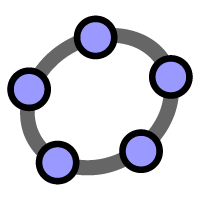
\includegraphics[scale=0.04]{img/introduction/geogebra-icon} if there is one.

When the program starts, the initial windows is shown (figure \ref{g:start-window}), allowing the user to choose among different working environments or \emph{Perspectives}.

\begin{figure}[h!]
\begin{center}
\includegraphics[width=\textwidth]{img/introduction/start-window}
\caption{Starting perspective of Geogegra.} \label{g:start-window}
\end{center}
\end{figure}

\section{Views}
Geogebra provides several windows that are called \emph{Views} and different working environments called \emph{Perspectives} that combine some views.
Both views and perspectives can be activated in the main menu of Geogebra that appears in the top right corner.
The most important views that we are going to use during these practices are:
\begin{description}
\item[Algebraic View] 
\includegraphics[scale=0.03]{img/introduction/algebraic-view-icon} This view allows to make algebraic and geometric constructions.
      It provides an \field{Input Bar} where the user can enter command and algebraic expressions.
      This is view is active by default when the program starts.
\item[Graphic View] 
\includegraphics[scale=0.03]{img/introduction/graphics-view-icon}
      This view allows to represent graphically geometric objects in the real plane.
      Beside the algebraic view, this view is also active by default when the program starts.
\item[3D Graphics View] 
\includegraphics[scale=0.3]{img/introduction/3d-graphics-view-icon} This view allows to represent graphically geometric objects in the real space.
      This view is not activated by default when the program starts, so that it must be activated by the user when it is required.
\item[CAS View] 
\includegraphics[scale=0.03]{img/introduction/cas-view-icon} (Computer Algebra System) This view allows to do symbolic calculations.
      It provides an \field{Input Bar} similar to the one of the algebraic view where you can enter commands and mathematical expressions, and evaluate them.
      This view is not activated by default when the program starts, but \emph{it will be the most used view during these practices}.
\end{description}


\section{Expression edition in the \field{CAS View}}
Before doing any computation with a mathematica expression, you need to know how to enter that expression and learn to manage it.


\subsection*{Entering expressions}
Any mathematical expression must be entered in the \field{Input Bar} of the \field{CAS View} (figure~\ref{g:input-bar}).

\begin{figure}[h!]
\begin{center}

\includegraphics[scale=0.6]{img/introduction/input-bar}
\caption{Input Bar.} \label{g:input-bar}
\end{center}
\end{figure}

The \field{Input Bar} allows to enter mathematical expressions, commands and text annotations.
In the mathematical expressions we can enter numbers, roman letters, greek letters, mathematical operators and any symbols that appears in the virtual keyboard.
It also allows to enter \LaTeX\footnote{\url{https://www.latex-project.org/}} code to format expressions.
For instance, it is possible to write superscripts with the command \command{\^{}} and subscripts with the command \command{\_}.

When the key \command{Enter} is pressed after entering a mathematical expression, Geogebra tries to evaluate it and it shows the result of the evaluation just below the expression, or a warning when there is some mistake in the expression.

Them most common operators for the construction of mathematical expressions are shown in the table below.

\begin{center}
\begin{tabular}{cc}
\tcrule
\textbf{Symbol} & \textbf{Operator} \\
\command{+}     & Addition          \\
\command{-}     & Subtraction       \\
\command{*}     & Product           \\
\command{/}     & Division          \\
\command{\^{}}  & Power             \\
\bcrule
\end{tabular}
\end{center}

At the time of writing a mathematical expression, you must take into account that Geogebra has an order of priority to evaluate the operators.
First it evaluates predefined functions and constants, after powers, after products and quotients (both with the same priority and from left to right), and finally additions and subtractions (both with the same priority and from left to right).
To force the evaluation of a subexpression, skipping the order of priority, you must use parenthesis.
Thus, as it can be appreciated in the table below, depending on how a expression is entered, you can get different results.

\begin{center}\renewcommand{\arraystretch}{2}
\begin{tabular}{cc}
\tcrule
\textbf{Entered expression} & \textbf{Evaluated expression} \\
\texttt{4x-1/x-5}           & $4x-\dfrac{1}{x}-5$           \\
\texttt{(4x-1)/x-5}         & $\dfrac{4x-1}{x}-5$           \\
\texttt{4x-1/(x-5)}         & $4x-\dfrac{1}{x-5}$           \\
\texttt{(4x-1)/(x-5)}       & $\dfrac{4x-1}{x-5}$           \\
\bcrule
\end{tabular}
\end{center}

Every expression that is entered in the \field{CAS View} is labelled with a number that allows to identify it.
Later, every time that we want to reference that expression we can use that identifier instead of writing again the whole expression.

There are two ways of referring to an expression, that are the static and the dynamic references.
To do a static reference we must write the symbol \# followed by the identifier number of the expression.
On the other hand, to do a dynamic reference we must write the symbol \$ followed by the identifier number of the expression.
A static reference will not change the expression where the reference is done even when the original expression changes, while for a dynamic reference, when the original expression changes, that change will be reflected in the expression where the reference is done.

It is possible to select any expression or subexpression of the \field{CAS View} and then copy and paste it in the \field{Input Bar}.


\subsection*{Entering text notes}
Geogebra also allows to enter text notes or comments int he \field{Input Bar}.
For that you have to right-click the \field{Input Bar} and select the option \option{Text} in the contextual menu that appears.
Text annotations are very helpful to explain the steps in a mathematical construction or to interpret the results.


\subsection*{Removing expressions}
Of course, it is possible to remove a expression from the \field{CAS View}.
For that you have to go to the line with the expression to remove and click the button 
\includegraphics[scale=0.035]{img/introduction/bin-button.png} or right-click that line and select the option \option{Delete row} in the contextual menu that appears.

If sometime we commit a mistake entering or deleting a wrong expression, it is possible to undo the last operations or redo them clicking the buttons 
\includegraphics[scale=0.03]{img/introduction/undo-button.png} or 
\includegraphics[scale=0.03]{img/introduction/redo-button.png} respectively.


\subsection*{Defining variables}
To define a variable we can use roman letters or greek letters.
The name of a variable can have more than one letter and, in this case, it is also possible to use numbers but it must start always by a letter.
Thus, for Geogebra, the expression \command{xy}, is not interpreted as the product of the variables $x$ and $y$, but the variable $xy$.
In addition, it distinguishes between upper and lower case, so that $xy$ and $xY$ are different variables.


\subsection*{Defining constants and functions}
To define a constant or a function the definition operator \command{:=} must be used.
To define a constant you have to write the name of the constant followed by \command{:=} and the value of the constant.
For example, to define the gravity constant we have to write \command{g:=9.81}.

On the other hand, to define a function you have to write the name of the function, followed buy the list of variables separated by commas and between parenthesis, then \command{:=} and finally the expression that defines the function.
For example, to define the function that calculates the area of triangle with base $b$ and high $h$, we have to write \command{a(b,h):=(b*h)/2} (ver figure~\ref{g:expressions}).


\begin{figure}[h!]
\begin{center}
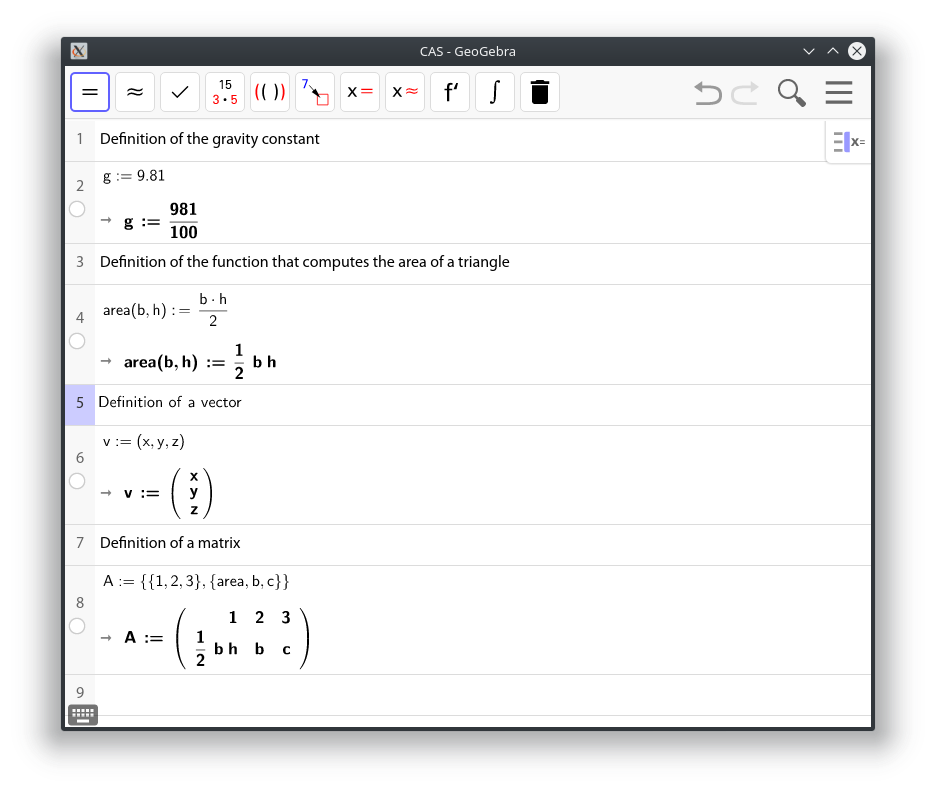
\includegraphics[scale=0.6]{img/introduction/math-expressions}
\caption{Entering mathematical expressions in the \field{Input Bar}.} \label{g:expressions}
\end{center}
\end{figure}


If we have defined a constant or function, and we change the definition after, the changes will be reflected in any other expression that contains the constant or function, except if the reference is static.

To remove a definition and free the name of the constant or function, for example \command{c}, we can use the command \command{Delete(c)} or the command \command{c:=}.


\subsection*{Predefined constants and functions}
Geogebra provides several predefined constants and functions that can be used in the mathematical expressions.
The sintax of some of these constants and functions is shown in the table~\ref{t:predefined-functions}, although, instead of using those commands, we can use the operators and constants of the virtual keyboard.

\begin{table}[h!]
\centering
\begin{tabular}{cl}
\tcrule
\textbf{Sintaxis}   & \textbf{Constante o función}                 \\
\command{pi}        & The number $\pi=3.14159\ldots$               \\
\command{Alt+e}     & Euler's constant $e=2.71828\ldots$           \\
\command{Alt+i}     & Imaginary number $i=\sqrt{-1}$               \\
\command{inf}       & Infinity $\infty$                            \\
\command{exp(x)}    & Exponential function $e^x$                   \\
\command{log(a,x)}  & Logarithmic function of base $a$, $\log_a x$ \\
\command{ln(x)}     & Neperian logarithmic function $\ln x$        \\
\command{sqrt(x)}   & Square root function $\sqrt{x}$              \\
\command{sin(x)}    & Sine function $\sin x$                       \\
\command{cos(x)}    & Cosine function $\cos x$                     \\
\command{tan(x)}    & Tangent function $\tan x$                    \\
\command{arcsin(x)} & Arcsine function $\arcsin x$                 \\
\command{arccos(x)} & Arccosine function $\arccos x$               \\
\command{arctan(x)} & Arctangent function $\arctan x$              \\
\bcrule
\end{tabular}
\caption{Sintax of some predefined constants and functions in Geogebra.} \label{t:predefined-functions}
\end{table}


\subsection*{Entering vectors and matrices}
Geogebra allows also to handle vectors and matrices.
To define a vector you must write its coordinates separated by commas between parenthesis.
For example, to enter the vector $(x,y,z)$ we have to write \command{(x,y,z)} (see figure~\ref{g:expressions}).

To define a matrix you must enter its elements by rows, separated by commas and between curly brackets.
For example, to enter the matrix
\[
\left(
\begin{array}{ccc}
1 & 2 & 3 \\
a & b & c \\
\end{array}
\right)
\]
we have to write \command{\{\{1,2,3\},\{a,b,c\}\}} (see figure~\ref{g:expressions}).


\subsection*{Simplifying expressions}
By default Geogebra always tries to simplify the mathematical expressions when it evaluates them.
For example, if you enter $x+x$ the result will be $2x$.
To avoid simplification you can change to the \button{Keep Input} mode clicking the button 
\includegraphics[scale=0.03]{img/introduction/keep-input-button}.

However, when Geogebra evaluates a mathematical expression it does not perform more complex simplifications, like, for instance, the simplification $\sin(x)^2+\cos(x)^2=1$.
To do this there are three commands:
\begin{description}
\item[Simplify] This is the most simple and tries to simplify a mathematical expression the most.
      For example, the command \command{Simplify(sin(x)\^{}2+cos(x)\^{}2)} returns \result{1}.
\item[Expand] This command tries to expand a mathematical expression computing all the possible powers, products, quotients, additions and subtractions.
      For example, the command \command{Expand((x+1)\^{}2)} returns \result{x\^{}2+2x+1}.
\item[Factor] This command tries to factorize a mathematical expression.
      For example, the command \command{Factoriza(x\^{}2+2x+1)} returns \result{(x+1)\^{}2}.
\end{description}

In any of these simplifications Geogebra uses by default the exact mode and returns fractional expressions.
To get the approximate value of a mathematical expression, with decimals, we must change to the \button{Numeric Evaluation} mode clicking the button 
\includegraphics[scale=0.03]{img/introduction/approximate-button}.
The number of decimal places showed can be set in the settings menu of Geogebra.

Lastly, it is possible to replace any variable by a value with the command \command{Substitute(<Expression>, <Substitution list>)}.
For example, the command \command{Substitute(2x+y, x=2, y=1)} returns \result{5}.


\subsection*{Entering equations and inequations}
To define equations in Geogebra the equality symbol \command{=} must be used.
Por example, the command \command{2x-y=1} defines the equation of a line.

And to define inequations we can use the symbols less than \command{<}, greater than \command{>}, less than or equal to \command{<=} or greater than or equal to \command{>=}.
For example, the command \command{x\^{}2+y\^{}2<=1} defines the circle with radius 1 centered at the origin.

To solve equations and inequation you can use the command \command{Solve(<equations>)}.
For example, the command \command{Solve(x\^{}2-5x+4=0)} returns \result{\{x=1, x=4\}}.
It is also possible to impose restrictions for the variables.
For example, the command \command{Solve(x\^{}2-5x+4=0, x>3)} returns only the solution \result{\{x=4\}}.

To solve systems of equations you must enter the list of equations separated by commans and between curly brackets.
For example, the command \command{Solve({2x+3=7, x-y=-1})} returns \result{\{x=3, y=2\}}.

This command also solves inequations.
For example, the command \command{Solve(3x-2<1)} returns \result{\{x<1\}}.


\section{Graphical representations}
One of the strengths of Geogebra is its graphics capabilities, sice it allows to represent graphically a lot of geometric objects both in the plane and in the real space.


\subsection*{Graphical representations in the real plane}
To represent geometric objects in the real plane $\mathbb{R}^2$, Geogebra uses the \field{Graphics View}.
By default any function defined in the \field{CAS View} will be plotted in this view.
To graphically represent other objects like constants, equations or inequations, it is required to click on the circle that appears to the left of the expression (see figure~\ref{g:graphics-view}).
To hide back the object in the \field{Graphics View} you have to click again on this circle.

\begin{figure}[h!]
\begin{center}
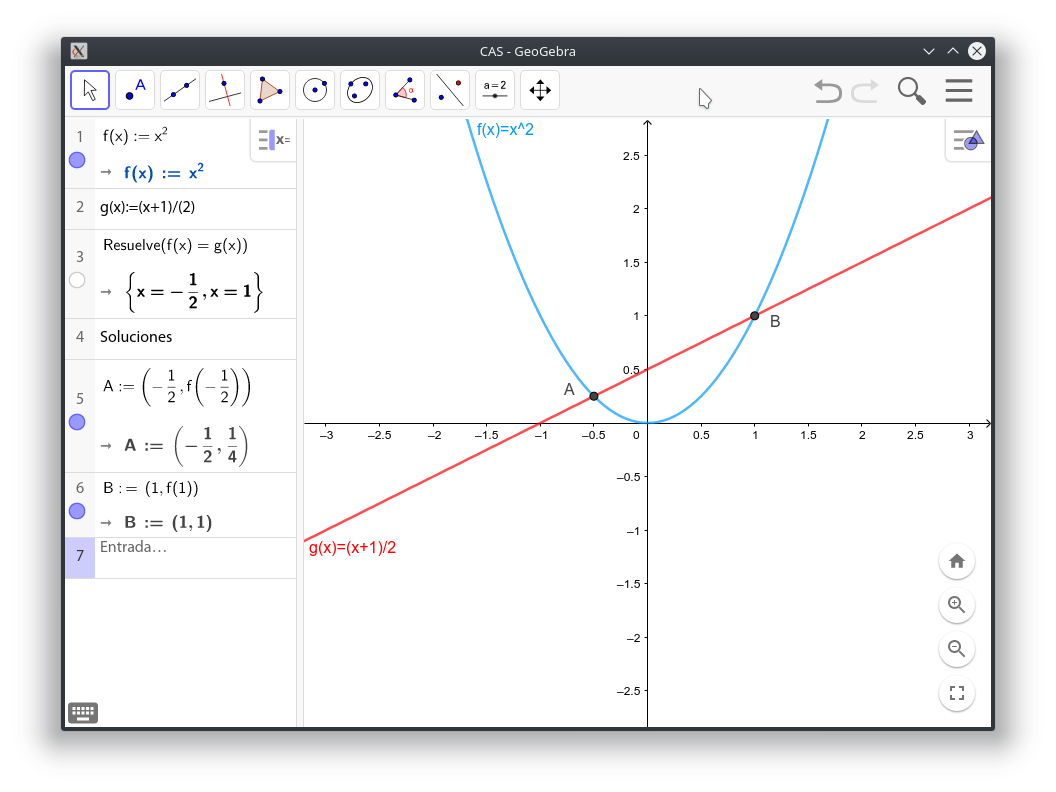
\includegraphics[width=\textwidth]{img/introduction/graphic-view}
\caption{Graphical representations in the \field{Graphics View}.} \label{g:graphics-view}
\end{center}
\end{figure}

Geogebra allows also the graphical representation of parametric functions defining the vector with the coordinate functions depending on one parameter.
For example, the command \command{g(t):=(cos(t), 2sin(t)cos(t))} plots the curve of the figure~\ref{g:parametric-curve}.

\begin{figure}[h!]
\begin{center}
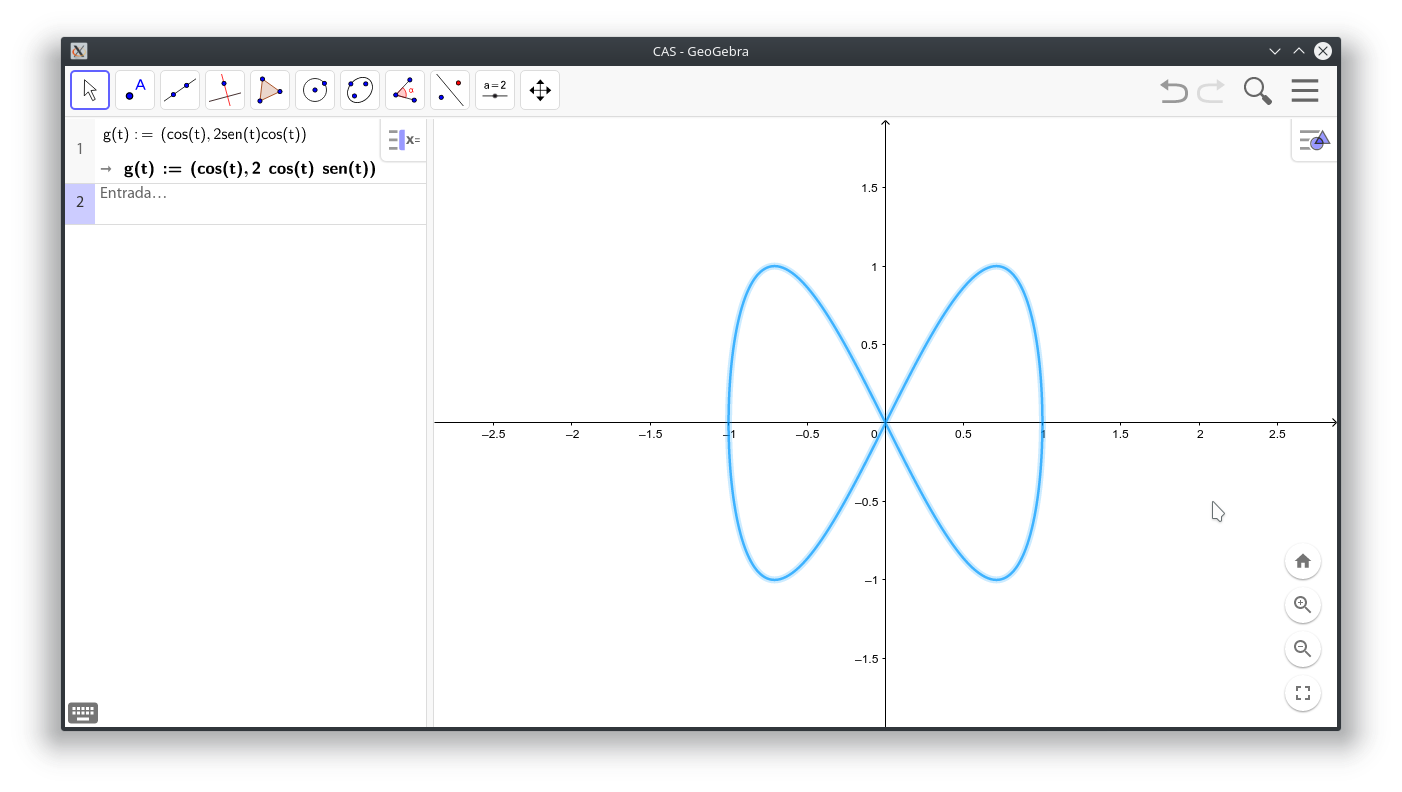
\includegraphics[width=\textwidth]{img/introduction/parametric-curve}
\caption{Graphical representation of a parametric curve in the real plane.} \label{g:parametric-curve}
\end{center}
\end{figure}

It is possible to change the aspect of any geometric object right-clicking on it and selecting the option \option{Settings} in the contextual menu that appears.
This opens a panel that allows to change the name of the object, the colour, the thickness or the opacity of the line, or even to enter a label that will appear next to the object in the \field{Graphics View}.

The \field{Graphics View} is centered at the origin of coordinates by default, but it is possible to make a zoom in or out clicking on the buttons 
\includegraphics[scale=0.03]{img/introduction/zoom-in-button} and 
\includegraphics[scale=0.03]{img/introduction/zoom-out-button} respectively.
It is also possible to move the view clicking at any position in the view and dragging the mouse.
To come back to the original view you can click on the button 
\includegraphics[scale=0.03]{img/introduction/home-button}.


\subsection*{Graphical representations in the real space}
To represent geometric objects in the real space $\mathbb{R}^3$, Geogebra uses the \field{3D Graphics View}.

By default, any function of two variables defined in the \field{CAS View} will be plotted in this view.
To graphically represent other objects like equations it is required to click on the circle that appears to the left of the expression (see figure~\ref{g:3D-graphics-view}).
Para ocultar de nuevo el objeto en la \field{Graphics View} basta con volver a hacer clic sobre ese círculo.

\begin{figure}[h!]
\begin{center}
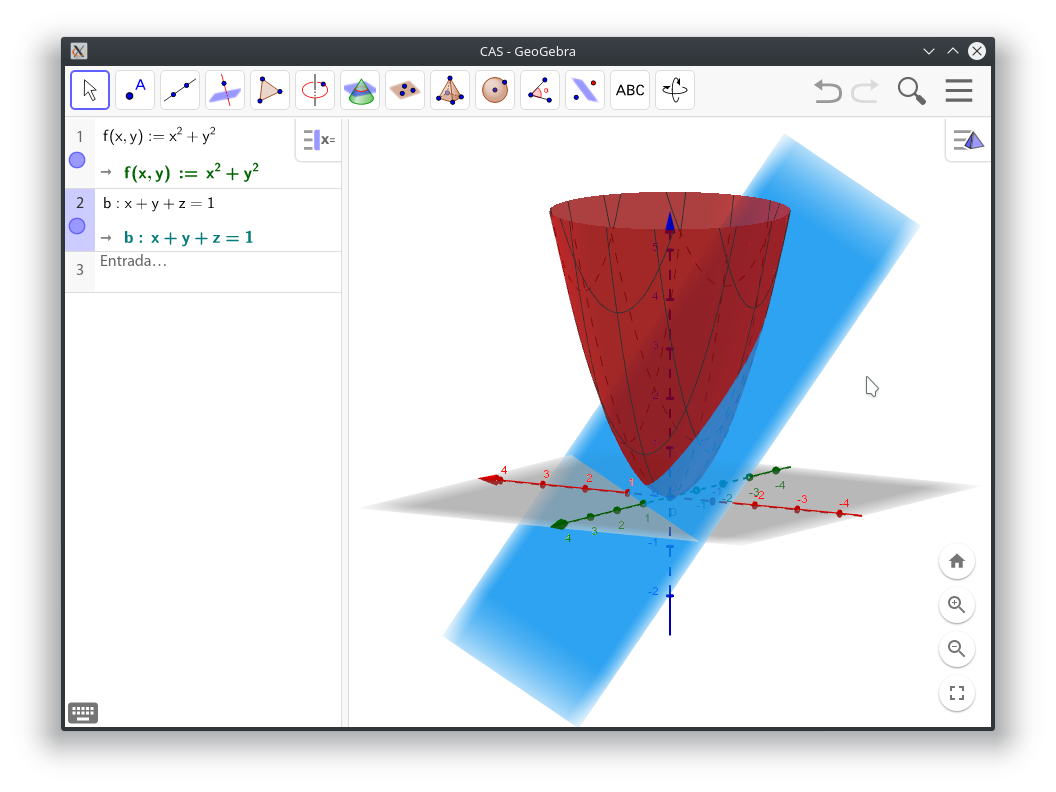
\includegraphics[width=\textwidth]{img/introduction/3D-graphic-view}
\caption{Grahpical representations in the \field{3D Graphics View}.} \label{g:3D-graphics-view}
\end{center}
\end{figure}

The same than in the \field{Graphics View} it is also possible to represent parametric functions defining the vector with the coordinate functions depending on one parameter.
For example, the command \command{h(t):=(cos(t), sin(t), t/2)} plots the curve of figure~\ref{g:3D-parametric-curve}.

\begin{figure}[h!]
\begin{center}
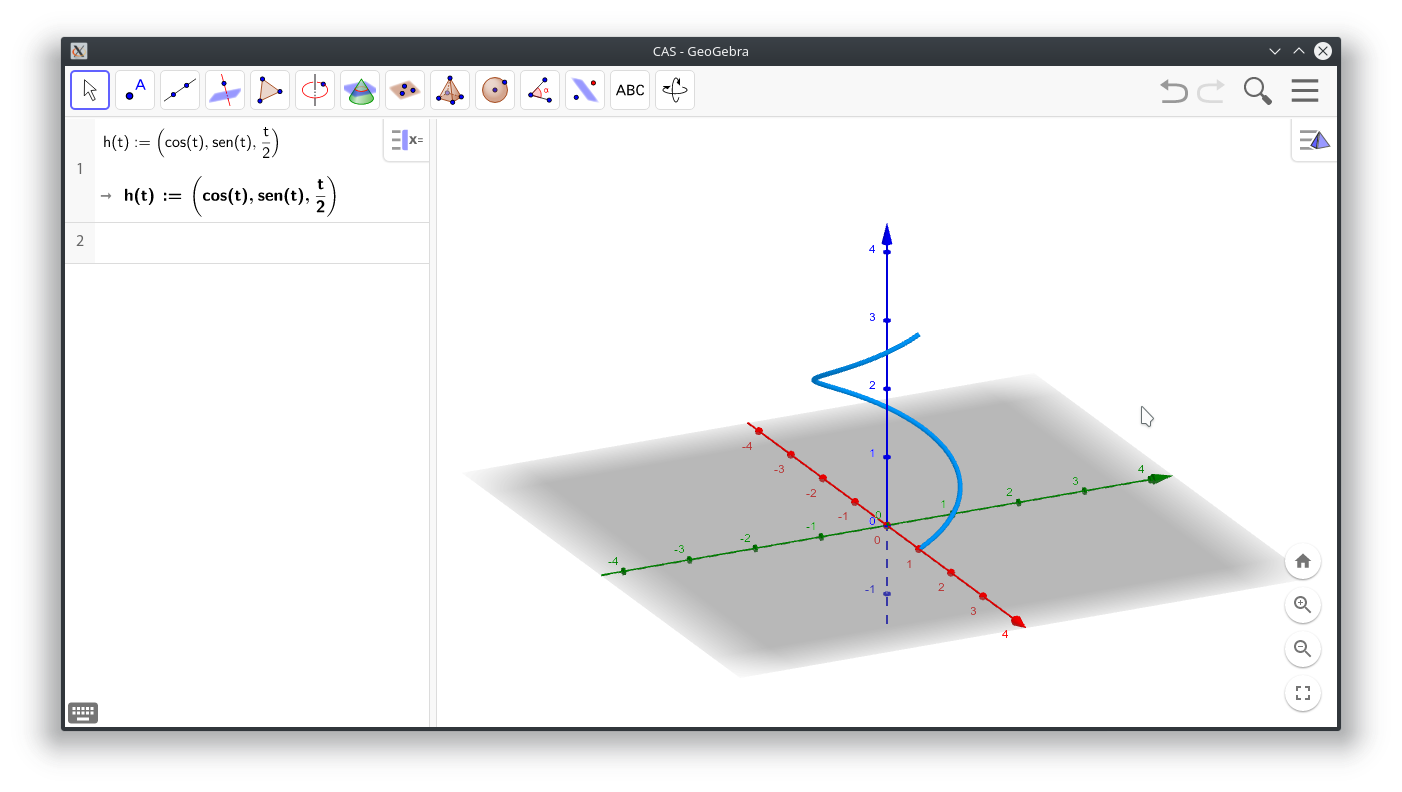
\includegraphics[width=\textwidth]{img/introduction/3D-parametric-curve}
\caption{Graphical representation of a parametric curve in the real space.} \label{g:3D-parametric-curve}
\end{center}
\end{figure}

The same than in the \field{Graphics View}, it is possible to change the aspect of any geometric object right-clicking on it and selecting the option \option{Settings} in the contextual menu that appears.
This opens a panel that allows to change the name of the object, the colour, the thickness or the opacity of the line, or even to enter a label that will appear next to the object in the \field{3D Graphics View}.

In the same way, it is possible to make a zoom in or out clicking on the buttons 
\includegraphics[scale=0.03]{img/introduction/zoom-in-button} and 
\includegraphics[scale=0.03]{img/introduction/zoom-out-button} respectively.
It is also possible to move the view with the button 
\includegraphics[scale=0.03]{img/introduction/move-button} or to rotate it with the button 
\includegraphics[scale=0.03]{img/introduction/rotate-button}.


\section{File management}
The mathematical expressions and calculus of the \field{CAS View} and the graphics of the \field{Graphics View} and \field{3D Graphics View} can be saved into a file.

\subsection*{Saving a file}
To save the mathematical expressions, calculus and graphics of a working session you must select the menu \menu{File>Save}.
If you have not logged in to the Geogebra web site a dialog appears asking for the user name an password to log in (see figure~\ref{g:login}).
If the you has no account in this site now is possible to register, but if you do not want to log in just click the link \button{Continue without signing in now}.

\begin{figure}[h!]
\begin{center}
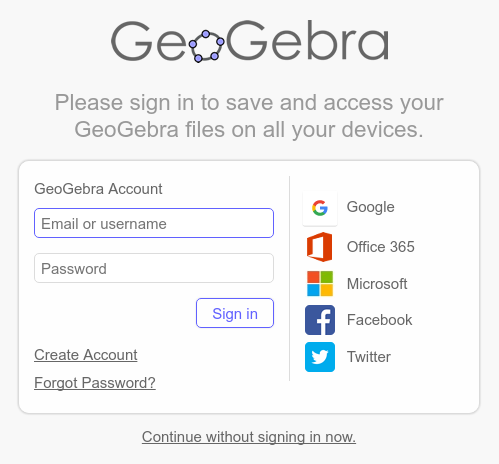
\includegraphics[scale=0.6]{img/introduction/login}
\caption{Login dialog of Geogebra web site.} \label{g:login}
\end{center}
\end{figure}

If you have logged in to the Geogebra web site, it will ask for the file name and the file will be uploaded to the Geogebra web site.
This way the file will be available whenever we are connected to this site with our user account.

If you have not logged in to the Geogebra web site, then a dialog is shown where you can enter the file name and select the local folder where to save the file in your computer.
Geogebras' files have extension \texttt{*.ggb}.

Once the file is saved, its name will appear in the title bar of the Geogebra window.


\subsubsection*{Opening a file}
To open a file in Geogebra you can use the menu \menu{File>Open}.
In the dialog shown you can choose to open a file from the Geogebra web site or to open a local file.

If you has logged in to the Geogebra web site, the files saved in our user account will appear automatically.
Eve if you are not logged in, you can open any public file in the Geogebra cloud.
For that we can search for a file entering a keyword in the search bar and Geogebra will show a list with all the files that contains that word.
Selecting any of them will download the file and open it.

If you want to open a local file you have to click on the folder icon.
This will open a dialog where you can select the file to open.


% \section{Printing}
% Geogebra permite imprimir las vistas gráficas seleccionando el menú \menu{Previsualización}.
% Tras esto aparece un cuadro de diálogo donde se puede seleccionar la ventana gráfica que se desea imprimir and las unidades de los ejes.
% Finalmente aparece el cuadro de diálogo de las impresoras donde hay que seleccionar la impresora con la que se quiere imprimir.

% También es posible exportar las vistas gráficas a diferentes formatos con el menú \menu{Descargar como}.
% Si se desea imprimir además de las gráficos las expresiones de la \field{CAS View} hay que seleccionar la opción \option{Construcción dinámica con página web (html)}.
% Esto genera una página web que puede abrirse con cualquier navegador and después imprimirse de la forma habitual.


\section{Solved exercises}
\begin{enumerate}
\item Enter and evaluate the following expressions.
      \begin{enumerate}
      \item $4x-\dfrac{1}{x}-5$.
            \begin{indication}
            Enter the expression \command{4x-1/x-5} in the \field{Input Bar} of the \field{CAS View}.
            \end{indication}
      \item $\dfrac{4x-1}{x}-5$.
            \begin{indication}
            Enter the expression \command{(4x-1)/x-5} in the \field{Input Bar} of the \field{CAS View}.
            \end{indication}
      \item $4x-\dfrac{1}{x-5}$.
            \begin{indication}
            Enter the expression \command{4x-1/(x-5)} in the \field{Input Bar} of the \field{CAS View}.
            \end{indication}
      \item $\dfrac{4x-1}{x-5}$.
            \begin{indication}
            Enter the expression \command{(4x-1)/(x-5)} in the \field{Input Bar} of the \field{CAS View}.
            \end{indication}
      \end{enumerate}

\item Define the following mathematical objects and plot them.
      \begin{enumerate}
      \item The constants $a=2$ and $b=3$.
            \begin{indication}
            \begin{enumerate}
            \item Enter the command \command{a:=2} in the \field{Input Bar} of the \field{CAS View} and activate the \field{Graphics View}.
            \item To plot the slider of the constant click the circle that appears to the left of the previous expression.
            \item Enter the command \command{b:=3} in the \field{Input Bar}.
            \item To plot the slider of the constant click the circle that appears to the left of the previous expression.
            \end{enumerate}
            \end{indication}
      \item The line $f(x)=a+bx$.
            Use the sliders of the constants to see how the line changes.
            \begin{indication}
            Enter the command \command{f(x):=a+b*x} in the \field{Input Bar}.
            \end{indication}
      \item The equation $ax^2+by^2=8$.
            Use the sliders of the constants to see how the conic changes.
            \begin{indication}
            Enter the command \command{a*x\^{}2+b*y\^{}2=8} in the \field{Input Bar}.
            \end{indication}
      \end{enumerate}

\item Define the following functions and plot them.
      \begin{enumerate}
      \item $f(x):=x^2$.
            \begin{indication}
            Enter the command \command{f(x):=x\^{}2} in the \field{Input Bar} of the \field{CAS View} and activate the \field{Graphics View}.
            \end{indication}
      \item $g(x):=\log(x)$.
            \begin{indication}
            Enter the command \command{g(x):=log(x)} in the \field{Input Bar}.
            \end{indication}
      \item $h(x):=\sin(x)$.
            \begin{indication}
            Enter the command \command{g(x):=sin(x)} in the \field{Input Bar}.
            \end{indication}
      \item $g\circ f(x)$.
            \begin{indication}
            Enter the command \command{g(f(x))} in the \field{Input Bar} and click the circle that appears to the left of the expression.
            \end{indication}
      \item $h\circ g \circ f(x)$.
            \begin{indication}
            Enter the command \command{h(g(f(x)))} in the \field{Input Bar} and click the circle that appears to the left of the expression.
            \end{indication}
      \item $f\circ g \circ h(x)$.
            \begin{indication}
            Enter the command \command{f(g(h(x)))} in the \field{Input Bar} and click the circle that appears to the left of the expression.
            \end{indication}
      \end{enumerate}

\item Given the matrices
      \[
      A=\left(
      \begin{array}{cc}
      a_{11} & a_{12} \\
      a_{21} & a_{22} \\
      a_{31} & a_{32}
      \end{array}
      \right)
      \qquad
      B=\left(
      \begin{array}{ccc}
      1 & 2 & 3 \\
      4 & 5 & 6
      \end{array}
      \right)
      \]
      and the vector $\mathbf{v}=(x, y, z)$, se pide:

      \begin{enumerate}
      \item Define the matrices $A$ and $B$, and the vector $v$.
            \begin{indication}
            \begin{enumerate}
            \item Enter the command \command{A:=\{\{a\_{11},a\_{12}\},\{a\_{21},a\_{22}\},\{a\_{31},a\_{32}\}\}} in the \field{Input Bar} of the \field{CAS View}.
            \item Enter the command \command{B:=\{\{1,2,3\},\{4,5,6\}\}} in the \field{Input Bar}.
            \item Enter the command \command{v:=(x,y,z)} in the \field{Input Bar}.
            \end{enumerate}
            \end{indication}
      \item Compute $A\cdot B$.
            \begin{indication}
            Enter the command \command{A*B} in the \field{Input Bar}.
            \end{indication}
      \item Compute $B\cdot A$.
            \begin{indication}
            Enter the command \command{B*A} in the \field{Input Bar}.
            \end{indication}
      \item Compute $\mathbf{v}\cdot A$.
            \begin{indication}
            Enter the command \command{v*A} in the \field{Input Bar}.
            \end{indication}
      \item Compute $B\cdot \mathbf{v}$.
            \begin{indication}
            Enter the command \command{B*v} in the \field{Input Bar}.
            \end{indication}
      \item Substitute $x=1$, $y=1$ and $z=0$ in the previous vector and plot it.
            \begin{indication}
            Enter the command \command{Substitute(\$,\{x=1,y=1,z=0\})} in the \field{Input Bar} and click the circle that appears to the left of the expression.
            \end{indication}
      \item Compute the modulus of the previous vector.
            \begin{indication}
            Enter the command \command{|\$|} in the \field{Input Bar} and click the circle that appears to the left of the expression.
            \end{indication}
      \item Change the previous substitution for $x=0$, $y=0$ and $z=1$ and observe how changes the modulus of the previous vector.
            \begin{indication}
            Edit the line with the substitution and change it for \command{Substitute(\$,\{x=0,y=0,z=1\})} in the \field{Input Bar}.
            \end{indication}
      \end{enumerate}

\item Find out the points where the graphs of the functions $f(x)=x^2$ and $g(x)=\dfrac{x+1}{2}$ intersect and plot them.
      \begin{enumerate}
      \item Enter the command \command{f(x):=x\^{}2} in the \field{Input Bar} of the \field{CAS View} and activate the \field{Graphics View}.
      \item Enter the command \command{g(x):=(x+1)/2} in the \field{Input Bar}.
      \item To solve the equation, enter the command \command{Solve(f=g)} in the \field{Input Bar}.
      \item To plot the intersection points, enter the command \command{Intersect(f,g)} in the \field{Input Bar} and click on the circle that appears to the left of the expression.
      \end{enumerate}

\item Plot the parametric function
      \[
      g(t)=
      \begin{cases}
      \cos(t) \\
      2\sin(t)\cos(t)
      \end{cases}
      t\in \mathbb{R}
      \]

      \begin{indication}
      Enter the command \command{g(t):=(cos(t), 2sin(t)cos(t))} in the \field{Input Bar} of the \field{CAS View} and activate the \field{Graphics View}.
      \end{indication}

\item Plot the following surfaces
      \[
      f(x,y)=\dfrac{2\sin(x^2+y^2)}{\sqrt{x^2+y^2}}, \qquad x^2+y 2+(z-2)^2=1
      \]
      and and the parametric curve
      \[
      h(t)=
      \begin{cases}
      \sin(t) \\
      \cos(t) \\
      t/2
      \end{cases}
      t\in \mathbb{R}
      \]
      \begin{indication}
      \begin{enumerate}
      \item Enter the command \command{f(x,y):=2sin(x\^{}2+y\^{}2)/sqrt(x\^{}2+y\^{}2)} in the \field{Input Bar} of the \field{CAS View} and activate the \field{3D Graphics View}.
      \item Enter the command \command{x\^{}2+y\^{}2+(z-2)\^{}2=1}  in the \field{Input Bar}.
      \item Enter the command \command{h(t):=(sin(t),cos(t),t/2)}  in the \field{Input Bar}.
      \end{enumerate}
      \end{indication}
\end{enumerate}
% !TEX root = ../practicas_geogebra.tex
% Author: Alfredo Sánchez Alberca (asalber@ceu.es)
\chapter{Elementary functions}

% \section{Fundamentos teóricos}

% En esta práctica se introducen los conceptos básicos sobre funciones reales de variable real, esto es, funciones
% \[f:\mathbb{R}\rightarrow \mathbb{R}.\]

% \subsection{Dominio e imagen}

% El \emph{Dominio} de la función $f$ es el conjunto de los números reales $x$ para los que existe $f(x)$ y se designa mediante $\dom f$.

% La \emph{Imagen} de $f$ es el conjunto de los números reales $y$ para los que existe algún $x\in \mathbb{R}$ tal que $f(x)=y$, y se denota por $\im f$.


% \subsection{Signo y crecimiento}
% El \emph{signo} de la función es positivo $(+)$ en los valores de $x$ para los que $f(x)>0$ y negativo $(-)$ en los que $f(x)<0$.
% Los valores de $x$ en los que la función se anula se conocen como \emph{raíces} de la función.

% Una función $f(x)$ es \emph{creciente} en un intervalo $I$ si $\forall\, x_1, x_2 \in I$ tales que $x_1<x_2$ se verifica que $f(x_1)\leq f(x_2)$.

% Del mismo modo, se dice que una función $f(x)$ es \emph{decreciente} en un intervalo $I$ si $\forall\, x_1, x_2 \in I$ tales que $x_1<x_2$ se verifica que $f(x_1)\geq f(x_2)$. En la figura~\ref{g:crecimiento} se muestran estos conceptos.

% \begin{figure}[h!]
% 	\centering \subfigure[Función creciente.] {\label{g:funcion_creciente}
% 		\scalebox{1}{\input{img/funciones_elementales/funcion_creciente}}}\qquad
% 	\subfigure[Función decreciente.]{\label{g:funcion_decreciente}
% 		\scalebox{1}{\input{img/funciones_elementales/funcion_decreciente}}}
% 	\caption{Crecimiento de una función.}
% 	\label{g:crecimiento}
% \end{figure}


% \subsection{Extremos Relativos}
% Una función $f(x)$ tiene un \emph{máximo relativo} en $x_0$ si existe un entorno $A$ de $x_0$ tal que $\forall x \in A$
% se verifica que $f(x)\leq f(x_0)$.

% Una función $f(x)$ tiene un \emph{mínimo relativo} en $x_0$ si existe un entorno $A$ de $x_0$ tal que $\forall x\in A$
% se verifica que $f(x)\geq f(x_0)$.

% Diremos que la función $f(x)$ tiene un \emph{extremo relativo} en un punto si tiene un \emph{máximo o mínimo relativo}
% en dicho punto. Estos conceptos se muestran en la figura~\ref{g:extremos}.

% \begin{figure}[h!]
% 	\centering \subfigure[Máximo relativo.] {\label{g:maximo}
% 		\scalebox{1}{\input{img/funciones_elementales/maximo}}}\qquad
% 	\subfigure[Mínimo relativo.]{\label{g:minimo}
% 		\scalebox{1}{\input{img/funciones_elementales/minimo}}}
% 	\caption{Extremos relativos de una función.}
% 	\label{g:extremos}
% \end{figure}

% Una función $f(x)$ está \emph{acotada superiormente} si $\exists K\in\mathbb{R}$ tal que $f(x)\leq K$ $\forall x \in \dom f$. Análogamente, se dice que una función $f(x)$ está \emph{acotada inferiormente} si $\exists K\in\mathbb{R}$ tal que $f(x)\geq K$ $\forall x \in \dom f$.

% Una función $f(x)$ está \emph{acotada} si lo está superior e inferiormente, es decir si $\exists K\in\mathbb{R}$ tal que $|f(x)|\leq K$ $\forall x \in \dom f$.


% \subsection{Concavidad}

% De forma intuitiva se puede decir que una función $f(x)$ es \emph{cóncava} en un intervalo $I$ si $\forall\, x_1, x_2
% \in I$, el segmento de extremos $(x_1,f(x_1))$ y $(x_2,f(x_2))$ queda por encima de la gráfica de $f$.

% Análogamente se dirá que es \emph{convexa} si el segmento anterior queda por debajo de la gráfica de $f$.

% Diremos que la función $f(x)$ tiene un \emph{punto de inflexión} en $x_0$ si en ese punto la función pasa de cóncava a
% convexa o de convexa a cóncava. Estos conceptos se ilustran en la figura~\ref{g:concavidad}.

% \begin{figure}[h!]
% 	\centering \subfigure[Función cóncava.] {\label{g:funcion_convexa}
% 		\scalebox{1}{\input{img/funciones_elementales/funcion_convexa}}}\qquad
% 	\subfigure[Función convexa.]{\label{g:funcion_concava}
% 		\scalebox{1}{\input{img/funciones_elementales/funcion_concava}}}
% 	\caption{Concavidad de una función.}
% 	\label{g:concavidad}
% \end{figure}

% \subsection{Asíntotas}

% La recta $x=a$ es una \emph{asíntota vertical} de la función $f(x)$ si al menos uno de los límites laterales de $f(x)$ cuando $x$ tiende hacia $a$ es $+\infty$ o $-\infty$, es decir cuando se verifique alguna de las siguientes igualdades
% \[
% 	\ \lim_{x\rightarrow a^{+}}f(x)=\pm\infty   \quad \textrm{o} \quad
% 	\lim_{x\rightarrow a^{-}}f(x)=\pm\infty
% \]

% La recta $y=b$ es una \emph{asíntota horizontal} de la función $f(x)$ si alguno de los límites de $f(x)$ cuando $x$ tiende hacia $+\infty$ o $-\infty$ es igual a $b$, es decir cuando se verifique
% \[
% 	\ \lim_{x\rightarrow -\infty }f(x)=b    \quad \textrm{o} \quad
% 	\ \lim_{x\rightarrow +\infty }f(x)=b
% \]

% La recta $y=mx+n$ es una \emph{asíntota oblicua} de la función $f(x)$ si alguno de los límites de $f(x)-(mx+n)$ cuando $x$ tiende hacia $+\infty$ o $-\infty$ es igual a 0, es decir si

% \[
% 	\ \lim_{x\rightarrow -\infty }{(f(x)-mx)}=n    \quad \textrm{o} \quad
% 	\ \lim_{x\rightarrow +\infty }{(f(x)-mx)}=n
% \]

% En la figura~\ref{g:asintotas} se muestran los distintos tipos de asíntotas.

% \begin{figure}[h!]
% 	\centering \subfigure[Asíntota horizontal y vertical.] {\label{g:asintotahorizontalyvertical}
% 		\scalebox{1}{\input{img/funciones_elementales/asintota_vertical}}}\qquad\qquad
% 	\subfigure[Asíntota vertical y oblicua.]{\label{g:asintotaoblicua}
% 		\scalebox{1}{\input{img/funciones_elementales/asintota_oblicua}}}
% 	\caption{Tipos de asíntotas de una función.}
% 	\label{g:asintotas}
% \end{figure}


% \subsection{Periodicidad}
% Una función $f(x)$ es \emph{periódica} si existe $h\in\mathbb{R^{+}}$ tal que \[f(x+h)=f(x)\  \forall x\in \dom f\] siendo el período $T$ de la función, el menor valor $h$ que verifique la igualdad anterior.

% En una función periódica, por ejemplo $f(x)=A\sin(wt)$, se denomina \emph{amplitud} al valor de $A$, y es la mitad de la diferencia entre los valores máximos y mínimos de la función. En la figura~\ref{g:periodoyamplitud} se ilustran estos conceptos.

% \begin{figure}[h!]
% 	\centering
% 	\scalebox{0.8}{\input{img/funciones_elementales/funcion_periodica}}
% 	\caption{Periodo y amplitud de una función periódica.}
% 	\label{g:periodoyamplitud}
% \end{figure}

% \clearpage
% \newpage

\section{Solved exercises}

\begin{enumerate}[leftmargin=*]
\item Consider the function
      \[
      f(t)=\frac{t^{4} +19t^{2} - 5}{t^{4} +9t^{2} - 10}.
      \]

      Representarla gráficamente y determinar a partir de dicha representación:

      \begin{enumerate}
      \item  Domain.
            \begin{indication}
            \begin{enumerate}
            \item Enter the expression \command{(t\^{}4+19t\^{}2-5)/(t\^{}4+9t\^{}2-10)} in the \field{Input Bar} of the \field{Vista CAS View} and activate the \field{Graphics View}.
            \item To determine the domain look at the values of $x$ where the function does exists, that is, where there is graph.
            \item Remember that, for this and the other parts of this exercise, we pretend to get approximate conclusions looking at the graph of the function.
            \end{enumerate}
            \end{indication}

      \item Image.
            \begin{indication}
            Look at the values of $y$ that are output of the function, that is, where there is graph.
            \end{indication}

      \item Asymtotes.
            \begin{indication}
            Look at the lines (horizontal, vertical or oblique) where the graph approaches (the distance between the graph and the line tends to zero as they tend to infinity).
            \end{indication}

      \item  Roots.
            \begin{indication}
            Look at the values of $x$ where the graph cuts the horizontal axis.
            \end{indication}

      \item Sign.
            \begin{indication}
            Look at the values of $x$ where the graph is over the horizontal axis (positive) and where it is under the horizontal axis (negative).

            \end{indication}

      \item Growth.
            \begin{indication}
            Look at the values of $x$ where $y$ increases when $x$ increases (increasing) and the values where $y$ decreases when $x$ increases (decreasing).
            \end{indication}

      \item Concavity.
            \begin{indication}
            Look at the values of $x$ where the curvature of the graph is up $\cup$ (concave up or convex) and where the curvature is $\cap$ (concave down or simply concave).
            \end{indication}

      \item Local extrema.
            \begin{indication}
            Look at the values of $x$ where the graph has a peak (relative maximum) and where the graph has a valley (relative minimum).
            \end{indication}

      \item Inflection points.
            \begin{indication}
            Look at the values of $x$ where the curvature changes continuously.
            \end{indication}
      \end{enumerate}

\item Representar en una misma gráfica las funciones $2^{x}, e^{x}, 0.7^{x}, 0.5^{x}$.
      A la vista de las gráficas obtenidas, ¿para qué valores de $a$ será la función creciente? ¿Y para qué valores de $a$ será decreciente?
      \begin{indication}
      \begin{enumerate}
      \item Introducir la función \command{2\^{}x} en la in the \field{Input Bar} of the \field{Vista CAS View}.
      \item Introducir la función \command{e\^{}x} en la \field{Barra de Entrada}.
      \item Introducir la función \command{0.7\^{}x} en la \field{Barra de Entrada}.
      \item Introducir la función \command{0.5\^{}x} en la \field{Barra de Entrada}.
      \item La función exponencial $a^x$ será creciente cuando $a>1$ y decreciente cuando $0<a<1$.
      \end{enumerate}
      \end{indication}

\item Representar en una misma gráfica las funciones siguientes, indicando su período y amplitud.
      \begin{enumerate}
      \item $\sin{x}$, $\sin{x}+2$, $\sin{(x+2)}$.
      \item $\sin{2x}$, $2\sin{x}$, $\sin\frac{x}{2}$.
            \begin{indication}
            \begin{enumerate}
            \item Introducir la función \command{sen(x)} en la in the \field{Input Bar} of the \field{Vista CAS View}.
            \item Introducir la función \command{sen(x)+2} en la \field{Barra de Entrada}.
            \item Introducir la función \command{sen(x+2)} en la \field{Barra de Entrada}.
            \item Introducir la función \command{sen(2x)} en la \field{Barra de Entrada}.
            \item Introducir la función \command{2sen(x)} en la \field{Barra de Entrada}.
            \item Introducir la función \command{sen(x/2)} en la \field{Barra de Entrada}.
            \end{enumerate}
            \end{indication}
      \end{enumerate}


\item Representar en una gráfica la función
      \[
      \ f(x)=\left\{
      \begin{array}{cl}
      -2x   & \hbox{si $x\leq0$;} \\
      x^{2} & \hbox{si $x>0$.}    \\
      \end{array}
      \right.
      \]

      \begin{indication}
      Introducir la función \command{Si(x<=0, -2x, x\^{}2)} en la \field{Barra de Entrada}.
      \end{indication}
\end{enumerate}


\section{Ejercicios propuestos}
\begin{enumerate}[leftmargin=*]
\item Hallar el dominio de las siguientes funciones a partir de sus representaciones gráficas:

      \begin{enumerate}
      \item $f(x)=\dfrac{x^{2} + x + 1}{x^{3} - x}$
      \item $g(x)=\sqrt[2]{x^{4}-1}$.
      \item $h(x)=\cos{\dfrac{x + 3}{x^{2} + 1}}$.
      \item $l(x)=\arcsin{\dfrac{x}{1+x}}$.
      \end{enumerate}

\item Se considera la función
      \[
      \ f(x)=\frac{x^{3} + x +2}{5x^{3} - 9x^{2} - 4x + 4}.
      \]

      Representarla gráficamente y determinar a partir de dicha representación:

      \begin{enumerate}
      \item Dominio.
      \item Imagen.
      \item Asíntotas.
      \item Raíces.
      \item Signo.
      \item Intervalos de crecimiento y decrecimiento.
      \item Intervalos de concavidad y convexidad.
      \item Extremos relativos.
      \item Puntos de inflexión.
      \end{enumerate}

\item Representar en una misma gráfica las funciones $\log_{10}{x}$, $\log_{2}{x}$, $\log{x}$, $\log_{0.5}{x}$.
      \begin{enumerate}
      \item A la vista de las gráficas obtenidas, indicar cuáles de las funciones anteriores son crecientes y cuáles son decrecientes.
      \item Determinar, a partir de los resultados obtenidos, o representando nuevas funciones si fuera necesario, para qué valores de $a$ será
            creciente la función $\log_{a}{x}$.
      \item Determinar, a partir de los resultados obtenidos, o representando nuevas funciones si fuera necesario, para qué valores de $a$ será
            decreciente la función $\log_{a}{x}$.
      \end{enumerate}

\item Completar las siguientes frases con la palabra igual, o el número de veces que sea mayor o menor en cada caso:
      \begin{enumerate}
      \item La función $\cos{2x}$ tiene un período............ que la función $\cos{x}$.
      \item La función $\cos{2x}$ tiene una amplitud............ que la función $\cos{x}$.
      \item La función $\cos\dfrac{x}{2}$ tiene un período............ que la función $\cos{3x}$.
      \item La función $\cos\dfrac{x}{2}$ tiene una amplitud............ que la función $\cos{3x}$.
      \item La función $3\cos{2x}$ tiene un período............ que la función $\cos\dfrac{x}{2}$.
      \item La función $3\cos{2x}$ tiene una amplitud............ que la función $\cos\dfrac{x}{2}$.
      \end{enumerate}

\item Hallar a partir de la representación gráfica, las soluciones de $e^{-1/x}=\dfrac{1}{x}$.

\item Representar en una gráfica la función
      \[
      \ f(x)=\left\{
      \begin{array}{ll}
      x^{3}   & \hbox{si $x<0$}    \\
      e^{x}-1 & \hbox{si $x\geq0$} \\
      \end{array}
      \right.
      \]

\end{enumerate}

% !TEX root = ../geogebra-practices.tex
% Author: Alfredo Sánchez Alberca (asalber@ceu.es)
\chapter{Limits and continuity}

% \section{Fundamentos teóricos}
% En esta práctica se introducen los conceptos de límite y continuidad de una función real, ambos muy relacionados.

% \subsection{Límite de una función en un punto}
% El concepto de límite está muy relacionado con el de proximidad y tendencia de una serie de valores. De manera informal, diremos que $l\in \mathbb{R}$ es el \emph{límite} de una función $f(x)$ en un punto $a\in \mathbb{R}$, si $f(x)$ tiende o se aproxima cada vez más a $l$, a medida que $x$ se aproxima a $a$, y se escribe
% \[ \lim_{x\rightarrow a} f(x)=l.\]

% Si lo que nos interesa es la tendencia de $f(x)$ cuando nos aproximamos al punto $a$ sólo por un lado, hablamos de \emph{límites laterales}. Diremos que $l$ es el \emph{límite por la izquierda} de una función $f(x)$ en un punto $a$, si $f(x)$ tiende o se aproxima cada vez más a $l$, a medida que $x$ se aproxima a $a$ por la izquierda, es decir con valores $x<a$, y se denota por
% \[ \lim_{x\rightarrow a^-} f(x)=l.\]
% Del mismo modo, diremos que $l$ es el \emph{límite por la derecha} de una función $f(x)$ en un punto $a$, si $f(x)$ tiende o se aproxima cada vez más a $l$, a medida que $x$ se aproxima a $a$ por la derecha, es decir con valores $x>a$, y se denota por
% \[ \lim_{x\rightarrow a^+} f(x)=l.\]

% Por supuesto, para que exista the limit global de la función $f(x)$ en el punto $a$, debe existir tanto the limit por la izquierda, como the limit por la derecha, y ser iguales, es decir
% \[
% \left.
% \begin{array}{l}
% \displaystyle \lim_{x\rightarrow a^-} f(x)=l \\
% \displaystyle \lim_{x\rightarrow a^+} f(x)=l
% \end{array}
% \right\}
% \Longrightarrow
% \lim_{x\rightarrow a} f(x)=l.
% \]

% \subsection{Álgebra de límites}
% Para el cálculo práctico de límites, se utiliza el siguiente
% teorema, conocido como Teorema de \emph{Álgebra de Límites}.


% 
% e $\lim_{x\rightarrow
% 
% , entonces se cumple
% 

% 

% 
% x)\pm g(x))=l_1\pm l_2$.
% 
% x)\cdot g(x))=l_1\cdot l_2$.
% 
% rac{f(x)}{g(x)}=\dfrac{l_1}{l_2}$ si $l_2\neq 0$.
% 
% mentales}


% \subsection{Así\input{capitulos/funciones_elementales}

% Como interpreta\input{capitulos/funciones_elementales}
% rica de los límites, definiremos rectas
% particulares a \input{capitulos/funciones_elementales}
% nde (se ``pega") la gráfica de una función
% cuando la varia\input{capitulos/funciones_elementales}
% a un cierto valor, finito o infinito.
% \subsubsection*\input{capitulos/funciones_elementales}
% verticales}
% La recta $x=a$ \input{capitulos/funciones_elementales}
% h{Asíntota Vertical} de la función $f(x)$
% si al menos uno\input{capitulos/funciones_elementales}
% ites laterales de $f$ en $a$ es $+\infty$
% ó $+\infty$. Es\input{capitulos/funciones_elementales}


% \[
% \mathop {\lim }\limits_{x \to a} f(x) =  \pm \infty
% \]

% \subsubsection*{Asíntotas Horizontales}
% La recta $y=b$ es una \emph{Asíntota Horizontal} de la función
% $f(x)$ si se cumple:
% \[
% \mathop {\lim }\limits_{x \to  + \infty } f(x) = b\quad
% \text{ó}\quad\mathop {\lim }\limits_{x \to  - \infty } f(x) = b
% \]


% \subsubsection*{Asíntotas Oblicuas}

% La recta $y=mx+n$, donde $m\neq0$, es \emph{Asíntota Oblicua} de la
% función $f(x)$ si:


% \[

% \m
% limits_{x \to  + \infty } \left[ {f(x) - \left( {mx
% + 
% ight] = 0\quad\text{ó}\quad\mathop {\lim }\limits_{x
% \t
% left[ {f(x) - \left( {mx + n} \right)} \right] = 0
% \]



% La
%  práctica de $m$ y $n$ se realiza del siguiente
% mo


% \[
% m = \mathop {\lim }\limits_{x \to  + \infty } \frac{{f(x)}} {x}
% \]

% \[
% n = \mathop {\lim }\limits_{x \to  + \infty } \left[ {f(x) - mx}
% \right]
% \]
% o bien lo mismo con los límites en $-\infty$:
% \[
% m = \mathop {\lim }\limits_{x \to  - \infty } \frac{{f(x)}} {x}
% \]

% \[
% n = \mathop {\lim }\limits_{x \to  - \infty } \left[ {f(x) - mx}
% \right]
% \]

% En cualquiera de los casos, si obtenemos un valor real para $m$ (no
% puede ser ni $+\infty$ ni $-\infty$) distinto de $0$, procedemos
% después a calcular $n$, que también debe ser real (sí que puede ser
% $0$).

% Si $m=\pm\infty$ entonces la función crece (decrece) más deprisa que
% cualquier recta, y si $m=0$ la función crece (decrece) más despacio
% que cualquier recta, y en cualquiera de los dos casos decimos que la
% función tiene una \emph{Rama Parabólica}.

% \subsection{Continuidad de una función en un punto}
% Diremos que una función $f(x)$ es continua en un punto $a\in
% \mathbb{R}$, si se cumple
% \[ \lim_{x\rightarrow a}f(x)=f(a),\]
% donde $f(a)\in \mathbb{R}$.

% La definición anterior implica a su vez que se cumplan estas tres
% condiciones:

% \begin{itemize}

% \item Existe the limit de $f$ en $x=a$.

% \item La función está definida en $x=a$; es decir, existe $f(a)$.

% \item Los dos valores anteriores coinciden.

% \end{itemize}

% Si la función $f$ no es continua en $x=a$, diremos que es
% \emph{discontinua} en el punto $a$, o bien que $f$ tiene una
% \emph{discontinuidad} en $a$.

% Intuitivamente, una función es continua cuando puede dibujarse su
% gráfica sin levantar el lápiz.

% \subsubsection*{Continuidad lateral en un punto}

% Si nos restringimos a los valores que toma una función a la derecha
% de un punto $x=a$, o a la izquierda, se habla de continuidad por la
% derecha o por la izquierda según la siguiente definición.

% Una función es \emph{continua por la derecha} en un punto $x=a$, y
% lo notaremos como $f$ continua en $a^+$, si existe the limit por la
% derecha en dicho punto y coincide con el valor de la función en el
% mismo:
% \[
% \mathop {\lim }\limits_{x \to a^ +  } f\left( x \right) = f\left( a
% \right)
% \]

% De igual manera, la función es \emph{continua por la izquierda} en
% un punto $x=a$, y lo notaremos como $f$ continua en $a^-$, si existe
% the limit por la izquierda en dicho punto y coincide con el valor de
% la función en el mismo:

% \[
% \mathop {\lim }\limits_{x \to a^ -  } f\left( x \right) = f\left( a
% \right)
% \]


% \subsubsection*{Propiedades de la continuidad en un punto}

% Como consecuencia de la definición de continuidad en un punto,
% podrían demostrarse toda una serie de teoremas, algunos de ellos
% especialmente importantes.

% \begin{itemize}

% \item \textbf{Álgebra de funciones continuas}.
%       Si $f$ y $g$ son funciones continuas en $x=a$, entonces $f\pm g$ y
%       $f\cdot g$ son también continuas en $x=a$. Si además $g(a)\neq 0$,
%       entonces $f/g$ también es continua en $x=a$.

% \item \textbf{Continuidad de funciones compuestas}. Si $f$ es continua en
%       $x=a$ y $g$ es continua en $b=f(a)$, entonces la función compuesta
%       $g\circ f$ es continua en $x=a$.

% \item \textbf{Continuidad y cálculo de límites}. Sean $f$ y $g$ dos
%       funciones tales que existe $\mathop {\lim }\limits_{x \to a} f(x) =
%       l$ $\in \mathbb{R}$ y $g$ es una función continua en $l$. Entonces:

%       \[
%       \mathop {\lim }\limits_{x \to a} g\left( {f\left( x \right)} \right)
%       = g\left( l \right)
%       \]

% \end{itemize}

% \subsubsection*{Tipos de discontinuidades}
% Puesto que la condición de continuidad puede no satisfacerse por
% distintos motivos, existen distintos tipos de discontinuidades:


% \begin{itemize}
% \item \textbf{Discontinuidad evitable}. Se dice que $f(x)$ tiene una \emph{discontinuidad evitable} en el punto $a$, si existe the limit de la función  pero no coincide con el valor de la función en el punto (bien porque sea diferente, bien por que la función no esté definida en dicho punto), es decir
%       \[\lim_{x\rightarrow a}f(x)=l\neq f(a).\]

% \item \textbf{Discontinuidad de salto}. Se dice que $f(x)$ tiene una \emph{discontinuidad de salto} en el punto $a$, si existe the limit de la función por la izquierda  y por la derecha pero son diferentes, es decir,
%       \[
%       \lim_{x\rightarrow a^-}f(x)=l_1\neq l_2=\lim_{x\rightarrow a^+}f(x).
%       \]
%       A la diferencia entre ambos límites $l_1-l_2$, se le llama
%       \emph{amplitud del salto}.

% \item \textbf{Discontinuidad esencial}. Se dice que $f(x)$ tiene una \emph{discontinuidad esencial} en el punto $a$, si no existe alguno de los límites laterales de la función.
% \end{itemize}

% \newpage

\section{Ejercicios resueltos}
\begin{enumerate}[leftmargin=*]
\item Given the function
      \[
      f(x)=\left( 1+\frac{2}{x}\right) ^{x/2},
      \]

      \begin{enumerate}
      \item Plot its graph and try to guess the values of the following limits looking at the graph:
            \begin{multicols}{2}
            \begin{enumerate}
            \item $\lim_{x\rightarrow -2^-} f(x)$
            \item $\lim_{x\rightarrow -2^+} f(x)$
            \item $\lim_{x\rightarrow -\infty} f(x)$
            \item $\lim_{x\rightarrow +\infty} f(x)$
            \item $\lim_{x\rightarrow 2} f(x)$
            \item $\lim_{x\rightarrow 0} f(x)$
            \end{enumerate}
            \end{multicols}

            \begin{indication}
            \begin{enumerate}
            \item To plot the graph, enter the function \command{f(x):=(1+2/x)\^{}(x/2)} in the \field{Input Bar} of the \field{CAS View} and activate the \field{Graphics View}.
            \item To guess the limits, create a slider entering the expression \command{a:=0} in the \field{Input Bar}.
            \item Enter the point \command{A:=(a,f(a))} to plot the point on the graph of the function.
            \item Finally, move the slider and observe the value of the $y$ coordinate when $x$ approaches any of the values in the limits.
            \end{enumerate}
            \end{indication}

      \item Compute the previous limits. Do you get the same results that you guess looking at the graph?
            \begin{indication}
            \begin{enumerate}
            \item To compute $\lim_{x\rightarrow -2^-} f(x)$ enter the command \command{LimitBelow(f(x), -2)} in the \field{Input Bar}.
            \item To compute $\lim_{x\rightarrow -2^+} f(x)$ enter the command \command{LimitAbove(f(x), -2)} in the \field{Input Bar}.
            \item To compute $\lim_{x\rightarrow -\infty} f(x)$ enter the command \command{Limit(f(x), -inf)} in the \field{Input Bar}.
            \item To compute $\lim_{x\rightarrow \infty} f(x)$ enter the command \command{Limit(f(x), inf)} in the \field{Input Bar}.
            \item To compute $\lim_{x\rightarrow 2} f(x)$ enter the command \command{Limit(f(x), 2)} in the \field{Input Bar}.
            \item To compute $\lim_{x\rightarrow 0} f(x)$ enter the command \command{Limit(f(x), 0)} in the \field{Input Bar}.
            \end{enumerate}
            \end{indication}
      \end{enumerate}

\item Given the function
      \[
      g(x)=
      \begin{cases}
      \dfrac{x}{x-2}    & \mbox{if $x\leq 0$;} \\
      \dfrac{x^2}{2x-6} & \mbox{if $x>0$;}
      \end{cases}
      \]
      \begin{enumerate}
      \item Plot the graph and determine graphically if there are asymptotes.
            \begin{indication}
            \begin{enumerate}
            \item To plot the graph, enter the function \command{g(x):=If(x<=0, x/(x-2), x\^{}2/(2x-6))} in the \field{Input Bar} of the \field{CAS View} and activate the \field{Graphics View}.
            \item To check if there are vertical, horizontal or oblique asymptotes look at the lines (horizontal, vertical or oblique) where the graph approaches (the distance between the graph and the line tends to zero as they tend to infinity).
            \end{enumerate}
            \end{indication}

      \item Compute the vertical asymptotes of $g$ and plot them if any.
            \begin{indication}
            \begin{enumerate}
            \item The function is not defined in the values where the denominators vanish.
                  To find the zeros of the denominator of the firt piece enter the command \command{Root(x-2)} in the \field{Input Bar}.
                  The only root is at $x=2$ but it falls outside the region of this piece.
            \item To find the zeros of the denominator of the second piece enter the command \command{Root(2x-6)} in the \field{Input Bar}.
                  The onliy root is at $x=3$, so that the function is not defined a that point and it could exist a vertical asymptote at this point.
            \item To check if there is a vertical asymptote a this point you have to compute the lateral limits  $\lim_{x\rightarrow 3^-}g(x)$ and $\lim_{x\rightarrow 3^+}g(x)$.
            \item To compute the lateral limit to the left enter the command \command{LimitBelow(g, 3)} in the \field{Input Bar}.
            \item To compute the lateral limit to the right enter the command \command{LimitAbove(g, 3)} in the \field{Input Bar}.
            \item Since $\lim_{x\rightarrow 3^-}g(x)=-\infty$ and $\lim_{x\rightarrow 3^+}g(x)=\infty$, there exist a vertical asymptote at $x=3$.
                  To plot it, enter the expression \command{x=3} in the \field{Input Bar}.
            \end{enumerate}
            \end{indication}

      \item Compute the horizontal asymptotes of $g$ and plot them if any.
            \begin{indication}
            \begin{enumerate}
            \item To check if there is an horizontal asymptote we have to compute the limits at infinity $\lim_{x\rightarrow -\infty} g(x)$ y $\lim_{x\rightarrow \infty} g(x)$.
            \item To compute the limit at $-\infty$ enter the command \command{Limit(g, -inf)} in the \field{Input Bar}.
            \item To compute the limit at $\infty$ enter the command \command{Limit(g, inf)} in the \field{Input Bar}.
            \item Since $\lim_{x\rightarrow -\infty} g(x)=1$, there exist an horizontal asymptote at $y=1$ to the left.
                  To plot it, enter the expression \command{y=1} in the \field{Input Bar}.
            \item Since $\lim_{x\rightarrow \infty} g(x)=\infty$, there is no horizontal asymptote to the right.
            \end{enumerate}
            \end{indication}

      \item Compute the oblique asymptotes of $g$ and plot them if any.
            \begin{indication}
            \begin{enumerate}
            \item To the left there is no asymptote since there is an horizontal asymptote.
                  To check if there is an oblique asymptote to the right you have to compute the limits $\lim_{x\rightarrow \infty}\frac{g(x)}{x}$.
                  For it, enter the \command{Limit(g/x, inf)} in the \field{Input Bar}.
            \item Since $\lim_{x\rightarrow \infty}\frac{g(x)}{x}=0.5$, there exist an oblique asymptote to the right and $0.5$.
            \item To compute the intercept you have to compute the limit $\lim_{x\rightarrow \infty}g(x)-0.5x$.
                  For it, enter the command \command{Limit(g(x)-0.5x, inf)} in the \field{Input Bar}.
            \item Since $\lim_{x\rightarrow \infty}g(x)-0.5x=1.5$ the equation of the oblique asymptote is $y=0.5x+1.5$.
                  To plot it, enter the expression \command{y=0.5x+1.5} in the \field{Input Bar}.
            \end{enumerate}
            \end{indication}
      \end{enumerate}

\item For the following functions determine the type of discontinuity at the points given.
      \begin{enumerate}
      \item  $f(x)=\dfrac{\sin x}{x}$ at $x=0$.

            \begin{indication}
            \begin{enumerate}
            \item To plot the graph enter the function \command{f(x):=sin(x)/x} in the \field{Input Bar} of the \field{CAS View} and activate the \field{Graphics View}.
            \item To compute the limit $\lim_{x\rightarrow 0^-}f(x)$ enter the command \command{LimitBelow(f, 0)} in the \field{Input Bar}.
            \item To compute the limit $\lim_{x\rightarrow 0^+}f(x)$ enter the command \command{LimitAbove(f, 0)} in the \field{Input Bar}.
            \item Since $\lim_{x\rightarrow 0^-}f(x)=\lim_{x\rightarrow 0^+}f(x)=1$, $f$ has a removable discontinuity at $x=0$.
            \end{enumerate}
            \end{indication}
      \item $g(x)=\dfrac{1}{2^{1/x}}$ at $x=0$.
            \begin{indication}
            \begin{enumerate}
            \item To plot the graph  enter the function \command{g(x):=1/2\^{}(1/x)} in the \field{Input Bar} of the \field{CAS View}.
            \item To compute the limit $\lim_{x\rightarrow 0^-}g(x)$ enter the command \command{LimitBelow(g, 0)} in the \field{Input Bar}.
            \item To compute the limit $\lim_{x\rightarrow 0^+}g(x)$ enter the command \command{LimitAbove(g, 0)} in the \field{Input Bar}.
            \item Since $\lim_{x\rightarrow 0^-}g(x)=\infty$, $g$ has an essential discontinuity at $x=0$.
            \end{enumerate}
            \end{indication}
      \item $h(x)=\dfrac{1}{1+e^{\frac{1}{1-x}}}$ at $x=1$.
            \begin{indication}
            \begin{enumerate}
            \item To plot the graph enter the function \command{h(x):=1/(1+e\^{}(1/(1-x)))} in the \field{Input Bar} of the \field{CAS View}.
            \item To compute the limit $\lim_{x\rightarrow 1^-}h(x)$ enter the command \command{LimitBelow(h, 1)} in the \field{Input Bar}.
            \item To compute the limit $\lim_{x\rightarrow 1^+}h(x)$ enter the command \command{LimitAbove(h, 1)} in the \field{Input Bar}.
            \item Since $\lim_{x\rightarrow 1^-}h(x)=0$ y $\lim_{x\rightarrow 1^+}f(x)=1$, $h$ has a jump discontinuity at $x=1$.
            \end{enumerate}
            \end{indication}
      \end{enumerate}


\item Plot the graph of the function
      \[
      f(x)=
      \left\{
      \begin{array}{ll}
      \dfrac{x+1}{x^2-1},       & \hbox{if $x<0$;}     \\
      \dfrac{1}{e^{1/(x^2-1)}}, & \hbox{if $x\geq 0$.} \\
      \end{array}
      \right.
      \]

      and determine the points where it has a discontinuity and classify them.

      \begin{indication}
      \begin{enumerate}
      \item To plot the graph enter the function \command{f(x):=If(x<0, (x+1)/(x\^{}2-1), 1/e\^{}(1/(x\^{}2-1)))} in the \field{Input Bar} of the \field{CAS View} and activate the \field{Graphics View}.
      \item First you have to find the points that are not in the domain for every piece.
            For it, you have to compute the zeros of the denominators that appears in any piece.
            To find the zeros of $x^2-1$ enter the command \command{Root(x\^{}2-1)} in the \field{Input Bar}.
      \item There are to roots at $x=-1$ and $x=1$.
            At this values the function is not defined and, therefore, is discontinuous.
            In addition to this points you have to study also what happens at $x=0$ where the definition of the function changes.
      \item To compute the limit $\lim_{x\rightarrow -1^-}f(x)$ enter the command \command{LimitBelow(f, -1)} in the \field{Input Bar}.
      \item To compute the limit $\lim_{x\rightarrow -1^+}f(x)$ enter the command \command{LimitAbove(f, -1)} in the \field{Input Bar}.
      \item Since $\lim_{x\rightarrow -1^-}f(x)=\lim_{x\rightarrow -1^+}f(x)=-0.5$, $f$ has a removable discontinuity at $x=-1$.
      \item To compute the limit $\lim_{x\rightarrow 0^-}f(x)$ enter the command \command{LimitBelow(f, 0)} in the \field{Input Bar}.
      \item To compute the limit $\lim_{x\rightarrow 0^+}f(x)$ enter the command \command{LimitAbove(f, 0)} in the \field{Input Bar}.
      \item Since $\lim_{x\rightarrow 0^-}f(x)=-1$ y $\lim_{x\rightarrow 0^+}f(x)=e$, $f$ has a jump discontinuity at $x=0$.
      \item To compute the limit $\lim_{x\rightarrow 1^-}f(x)$ enter the command \command{LimitBelow(f, 1)} in the \field{Input Bar}.
      \item To compute the limit $\lim_{x\rightarrow 1^+}f(x)$ enter the command \command{LimitAbove(f, 1)} in the \field{Input Bar}.
      \item Since $\lim_{x\rightarrow 1^-}f(x)=\infty$, $f$ has an essential discontinuity at $x=1$.
      \end{enumerate}
      \end{indication}
\end{enumerate}


\section{Ejercicios propuestos}
\begin{enumerate}[leftmargin=*]
\item Compute the following limits:
      \begin{multicols}{2}
      \begin{enumerate}
      \item $\displaystyle \lim_{x\rightarrow 1}\dfrac{x^3-3x+2}{x^4-4x+3}$.
      \item $\displaystyle \lim_{x\rightarrow a}\dfrac{\sin x-\sin a}{x-a}$.
      \item $\displaystyle \lim_{x\rightarrow\infty}\dfrac{x^2-3x+2}{e^{2x}}$.
      \item $\displaystyle \lim_{x\rightarrow\infty}\dfrac{\log(x^2-1)}{x+2}$.
      \item $\displaystyle \lim_{x\rightarrow 1}\dfrac{\log(1/x)}{\tan(x+\dfrac{\pi}{2})}$.
      \item $\displaystyle \lim_{x\rightarrow a}\dfrac{x^n-a^n}{x-a}\quad n\in \mathbb{N}$.
      \item $\displaystyle \lim_{x\rightarrow 1}\dfrac{\sqrt[n]{x}-1}{\sqrt[m]{x}-1}\quad n,m \in \mathbb{Z}$.
      \item $\displaystyle \lim_{x\rightarrow 0}\dfrac{\tan x-\sin x}{x^3}$.
      \item $\displaystyle \lim_{x\rightarrow \pi/4}\dfrac{\sin x-\cos x}{1-\tan x}$.
      \item $\displaystyle \lim_{x\rightarrow 0}x^2e^{1/x^2}$.
      \item $\displaystyle \lim_{x\rightarrow \infty}\left(1+\dfrac{a}{x}\right)^x$.
      \item $\displaystyle \lim_{x\rightarrow 0}\left(\dfrac{1}{x}\right)^{\tan x}$.
      \item $\displaystyle \lim_{x\rightarrow 0}(\cos x)^{1/\mbox{\footnotesize sen}\, x}$.
      \item $\displaystyle \lim_{x\rightarrow 0}\dfrac{6}{4+e^{-1/x}}$.
      \item $\displaystyle \lim_{x\rightarrow \infty}\left(\sqrt{x^2+x+1}-\sqrt{x^2-2x-1}\right)$.
      \end{enumerate}
      \end{multicols}

\item Given the function
      \[
      f(x) =
      \begin{cases}
      \dfrac{x^2+1}{x+3}       & \mbox{if $x<0$};     \\
      \dfrac{1}{e^{1/(x^2-1)}} & \mbox{if $x\geq 0$;}
      \end{cases}
      \]
      compute its asymptotes.

\item The following functions are not defined at $x=0$.
      Determine, when possible, the value that should take the function at that point to be continuous.
      \begin{multicols}{2}
      \begin{enumerate}
      \item $f(x)=\dfrac{(1+x)^n-1}{x}$.
      \item $h(x)=\dfrac{e^x-e^{-x}}{x}$.
      \item $j(x)=\dfrac{\log(1+x)-\log(1-x)}{x}$.
      \item $k(x)=x^2\sin\dfrac{1}{x}$.
      \end{enumerate}
      \end{multicols}

\end{enumerate}

% !TEX root = ../geogebra-practices.tex
% Author: Alfredo Sánchez Alberca (asalber@ceu.es)
\chapter{Derivatives of functions of one variable}

% \section{Fundamentos teóricos}
% El concepto de derivada es uno de los más importantes del Cálculo
% pues resulta de gran utilidad en el estudio de funciones y tiene
% multitud de aplicaciones. En esta práctica introducimos este
% concepto y presentamos algunas de sus aplicaciones, tanto en
% funciones de una como de varias variables.

% \subsection{Tasas de variación media e instantánea. La derivada}
% Cuando queremos conocer la variación que experimenta una función
% real $f(x)$ en un intervalo $[a,b]$, se calcula la diferencia
% $f(b)-f(a)$ que se conoce como \emph{incremento} de $f$, y se nota
% $\Delta f[a,b]$, aunque, a veces, simplemente se escribe $\Delta f$.

% En muchas otras ocasiones veces resulta importante comparar la
% variación que experimenta la función $f$ con relación a la variación
% que experimenta su argumento $x$ en un intervalo $[a,b]$. Si tenemos
% en cuenta que $b=a+\Delta x$, esto viene dado por la \emph{tasa de
% variación media}, que se define como:

% \[
% \textrm{TVM} f[a,b]=\textrm{TVM} f[a,a+\Delta x]=\frac{\Delta
% f}{\Delta x}=\frac{f(b)-f(a)}{b-a}=\frac{f(a+\Delta x )-f(a)}{\Delta
% x}. 
% \]

% También resulta muy común llamar a $\Delta x$ con la letra $h$, por
% lo que la expresión anterior queda de la forma:

% \[
% \textrm{TVM} f[a,b]=\textrm{TVM} f[a,a+h]=\frac{\Delta f}{\Delta
% x}=\frac{f(a+h)-f(a)}{h}.
% \]

% Desde el punto de vista geométrico, la tasa de variación media de
% $f$ en el intervalo $[a , a+\Delta x]$ es la pendiente de la recta
% secante a $f$ en los puntos $(a , f(a))$ y $(a+\Delta x, f(a+\Delta
% x))$, tal y como se muestra en la figura~\ref{g:secante}.

% \begin{figure}[h!]
% \begin{center}
% \scalebox{1}{\input{img/derivadas/secante}}
% \caption{La tasa de variación media como la pendiente de la recta
% secante a una función en dos puntos.} \label{g:secante}
% \end{center}
% \end{figure}


% Y, a veces, incluso más importante que la tasa de variación media,
% es estudiar la tasa de variación que experimenta la función, no en
% un intervalo, sino en un punto, tomando para ello límites cuando el
% incremento en la variable independiente tiende 0. Definimos la tasa
% de variación de una función en un punto $a$, o también tasa de
% variación instantánea, a partir de la tasa de variación media de la
% función en el intervalo $[a,a+\Delta x]$. Dicha tasa, si existe,
% recibe el nombre de \emph{derivada} de la función real $f(x)$ en un
% punto $a\in \mathbb{R}$, y se nota como $f'(a)$, o bien
% $\dfrac{df}{dx}(a)$:

% \[
% f'(a)=\dfrac{df}{dx}(a)= \lim_{\Delta x\rightarrow 0}\frac{\Delta
% f}{\Delta x}=\lim_{\Delta x\rightarrow 0}\frac{f(a+\Delta
% x)-f(a)}{\Delta x}=\lim_{h\rightarrow 0}\frac{f(a+h)-f(a)}{h}.
% \]

% Cuando este límite existe, se dice que la función $f$ es
% \emph{derivable} o \emph{diferenciable} en el punto $a$.

% Geométricamente, $f'(a)$ es la pendiente de la recta tangente a la
% curva de $f(x)$ en el punto $(a,f(a))$, tal y como se aprecia en la
% figura~\ref{g:tangente}.

% \begin{figure}[h!]
% \begin{center}
% \scalebox{1}{\input{img/derivadas/tangente}}
% \caption{La derivada como la pendiente de la recta tangente a una
% función en un punto.} \label{g:tangente}
% \end{center}
% \end{figure}

% \subsubsection*{Recta tangente y normal a una función en un punto}
% De la gráfica anterior, fácilmente se deduce que la ecuación de la
% recta tangente a una función $f(x)$ en el punto $(a,f(a))$ es:
% \[
% y=f(a)+f'(a)(x-a).
% \]

% Y teniendo en cuenta que la pendiente de la recta normal (recta
% perpendicular a la recta tangente) es la inversa cambiada de signo,
% la ecuación de la recta normal a $f(x)$ en el punto $(a,f(a))$ es:
% \[
% y=f(a)-\frac{1}{f'(a)}(x-a).
% \]

% \subsection{Función derivada y derivadas sucesivas}

% El límite que nos sirve para calcular la derivada de una función en
% un punto, define una nueva función $f'$ cuyo dominio está formado
% por los puntos en los que $f$ es diferenciable. La función $f'(x)$,
% o también $\dfrac{df}{dx}$, se llama \emph{primera derivada} de $f$.

% Puesto que $f'$ es una función, puede derivarse a su vez, y la
% primera derivada de $f'$ se conoce como segunda derivada de $f$, y
% se nota $f''(x)$ o $\dfrac{d^2f}{dx^2}$. Análogamente, la
% \emph{$n$-ésima derivada} de $f$, designada por $f^{(n}$ o
% $\dfrac{d^nf}{dx^n}$, es la primera derivada de $f^{(n-1}$, para
% $n=2,3,\ldots$, es decir
% \[
% \frac{d^nf}{dx^n}=\frac{d}{dx}\left(\frac{d^{n-1}f}{dx^{n-1}}\right)\
% n=2,3,\ldots
% \]


% \subsection{Estudio del crecimiento de una función}
% Una función $f(x)$ es \emph{creciente} en un intervalo $I$ si
% $\forall\, x_1, x_2 \in I$ tales que $x_1<x_2$ se verifica que
% $f(x_1)\leq f(x_2)$.

% Del mismo modo, se dice que una función $f(x)$ es \emph{decreciente}
% en un intervalo $I$ si $\forall\, x_1, x_2 \in I$ tales que
% $x_1<x_2$ se verifica que $f(x_1)\geq f(x_2)$. En la
% figura~\ref{g:crecimiento_derivada} se muestran estos conceptos.

% \begin{figure}[h!]
% \centering \subfigure[Función creciente.] {\label{g:funcion_creciente}
% \scalebox{1}{\input{img/funciones_elementales/funcion_creciente}}}\qquad
% \subfigure[Función decreciente.]{\label{g:funcion_decreciente}
% \scalebox{1}{\input{img/funciones_elementales/funcion_decreciente}}}
% \caption{Crecimiento de una función.}
% \label{g:crecimiento_derivada}
% \end{figure}

% Si $f$ es una función derivable en el intervalo $I$, el signo de la
% derivada puede utilizarse para estudiar el crecimiento de la función
% ya que se cumple:
% \begin{itemize}
% \item $f$ es creciente en $x_0\in I$, si y sólo si, $f'(x_0)\geq 0$.
% \item $f$ es decreciente en $x_0\in I$, si y sólo si, $f'(x_0)\leq 0$.
% \end{itemize}

% Desde el punto de vista geométrico, esto es evidente, ya en los
% intervalos donde $f$ es creciente, cualquier recta tangente tiene
% pendiente positiva, mientras que en los intervalos donde $f$ es
% decreciente, las tangentes tienen pendiente negativa, tal y como se
% observa en la figura~\ref{g:crecimiento_derivada}.

% \subsection{Determinación de los extremos relativos}
% Una función $f(x)$ tiene un \emph{máximo relativo} en $x_0$ si
% existe un entorno $A$ de $x_0$ tal que $\forall x \in A$ se verifica
% que $f(x)\leq f(x_0)$.

% Una función $f(x)$ tiene un \emph{mínimo relativo} en $x_0$ si
% existe un entorno $A$ de $x_0$ tal que $\forall x\in A$ se verifica
% que $f(x)\geq f(x_0)$.

% Diremos que la función $f(x)$ tiene un \emph{extremo relativo} en un
% punto si tiene un \emph{máximo o mínimo relativo} en dicho punto.

% Cuando $f$ es una función continua, entonces también se puede
% definir un extremo relativo como aquel punto donde cambia el
% crecimiento de la función. Así, un máximo relativo es un punto donde
% la función pasa de ser creciente a ser decreciente, y un mínimo
% relativo es un punto donde la función pasa de ser decreciente a ser
% creciente, tal y como se muestra en la figura~\ref{g:extremos_derivada}.

% \begin{figure}[h!]
% \centering \subfigure[Máximo relativo.] {\label{g:maximo}
% \scalebox{1}{\input{img/funciones_elementales/maximo}}}\qquad
% \subfigure[Mínimo relativo.]{\label{g:minimo}
% \scalebox{1}{\input{img/funciones_elementales/minimo}}}
% \caption{Extremos relativos de una función.}
% \label{g:extremos_derivada}
% \end{figure}

% Si $f$ tiene un extremo relativo en un punto $x_0$ y existe la
% derivada en dicho punto, entonces se cumple que $f'(x_0)=0$, es
% decir, la tangente a la gráfica de $f$ en dicho punto es horizontal
% (figura~\ref{g:extremos_derivada}). El recíproco no es cierto en general, de
% modo que esta es una condición necesaria pero no suficiente. No
% obstante, si $f$ es una función derivable en un intervalo $I$,
% podemos utilizar esta propiedad para detectar los puntos entre los
% que se encontrarán los extremos relativos del intervalo $I$. Los
% puntos donde se anula la primera derivada, se conocen como
% \emph{puntos críticos} y serán candidatos a extremos. Una vez
% detectados los puntos críticos, para ver si se trata de un extremo
% relativo o no, basta con estudiar el crecimiento de la función a la
% izquierda y a la derecha del punto tal y como se indicaba en la
% sección anterior. Resumiendo, si $f'(x_0)=0$, entonces:
% \begin{itemize}
% \item Si existe un $\delta>0$ tal que $f'(x)>0\ \forall\, x\in (x_0-\delta,x_0)$ (derivada positiva a la izquierda de $x_0$) y $f'(x)<0\ \forall\, x\in (x_0,x_0+\delta)$ (derivada negativa a la derecha de $x_0$), $x_0$ es un máximo relativo.

% \item Si existe un $\delta>0$ tal que $f'(x)<0\ \forall\, x\in (x_0-\delta,x_0)$ (derivada negativa a la izquierda de $x_0$) y $f'(x)>0\ \forall\, x\in (x_0,x_0+\delta)$ (derivada positiva a la derecha de $x_0$), $x_0$ es un mínimo relativo.

% \item En cualquier otro, $x_0$ es un \emph{punto de inflexión}.
% \end{itemize}

% \subsection{Estudio de la concavidad de una función}
% Se dice que una función $f(x)$ es \emph{cóncava} en un intervalo $I$
% si $\forall\, x_1, x_2 \in I$, el segmento de extremos
% $(x_1,f(x_1))$ y $(x_2,f(x_2))$ queda por encima de la gráfica de
% $f$.

% Análogamente se dirá que es \emph{convexa} si el segmento anterior
% queda por debajo de la gráfica de $f$.

% Diremos que la función $f(x)$ tiene un \emph{punto de inflexión} en
% $x_0$ si en ese punto la función pasa de cóncava a convexa o de
% convexa a cóncava. Estos conceptos se ilustran en la
% figura~\ref{g:concavidad_derivada}.

% \begin{figure}[h!]
% \centering \subfigure[Función cóncava.] {\label{g:funcion_concava_arriba}
% \scalebox{1}{\input{img/funciones_elementales/funcion_concava_arriba}}}\qquad
% \subfigure[Función convexa.]{\label{g:funcion_concava_abajo}
% \scalebox{1}{\input{img/funciones_elementales/funcion_concava_abajo}}}
% \caption{Concavidad de una función.}
% \label{g:concavidad_derivada}
% \end{figure}


% Si $f$ es una función derivable en el intervalo $I$, el signo de la
% segunda derivada puede utilizarse para estudiar la concavidad de la
% función ya que se cumple:
% \begin{itemize}
% \item $f$ es cóncava en $x_0\in I$, si y sólo si, $f''(x_0)\geq 0$.
% \item $f$ es convexa en $x_0\in I$, si y sólo si, $f''(x_0)\leq 0$.
% \end{itemize}

% \newpage

\section{Solved exercises}
\begin{enumerate}[leftmargin=*]
% \item Given the function $f(x)=\dfrac{x^3+x^2-2x-2}{x+3}$, se pide:
% \begin{enumerate}
% \item Calcular la tasa de variación media de $f$ en los intervalos $[-1,3]$, $[-1,0]$ y $[-1,-0.5]$, y calcular las correspondientes rectas
% secantes.
% \begin{indication}
% \begin{enumerate}
% \item To compute la tasa de variación media, definir previamente la función, y luego, por ejemplo para el intervalo $[-1,3]$, aplicamos
% la fórmula vista en la teoría:
% \[
% \textrm{TVM} f[-1,3]=\frac{\Delta y}{\Delta
% x}=\frac{f(3)-f(-1)}{3-(-1)}.
% \]
% \item To compute la ecuación de la recta secante, podemos utilizar, por ejemplo, la ecuación de la recta de la que conocemos un punto por
% el que pasa, $(x_0,y_0)$ y su pendiente, $m$:
% \[
% y - y_0  = m\left( {x - x_0 } \right)
% \]
% En nuestro caso, para el primero de los intervalos considerados, el punto puede ser, por ejemplo el $(-1,f(-1))$; y la pendiente viene dada
% por la tasa de variación media de la función en dicho intervalo. Es decir, la recta que buscamos tendrá como ecuación:
% \[
% y - f( - 1) = \textrm {TVM} f[ - 1,3]\left( {x - ( - 1)} \right)
% \]
% \item Después de calcular la ecuación de la recta secante, podemos comprobar que la misma corta a la función en los puntos adecuados sin más
% que representar en la misma gráfica tanto $f$ como la recta calculada.
% \end{enumerate}
% \end{indication}
% 
% 
% \item Calcular la tasa de variación instantánea de $f$ en el punto $-1$ haciendo uso de límites, y calcular la correspondiente recta
% tangente.
% \begin{indication}
% \begin{enumerate}
% \item Como ya sabemos por la teoría, las tasa de variación instantánea de la función en un punto dado si existe, recibe el nombre de
% derivada de la función en el punto, y se calcula mediante the limit:
% \[
% f'(a) = \mathop {\lim }\limits_{h \to 0} \frac{{f(a + h) - f(a)}}
% {h}
% \]
% en donde, por aligerar la notación, hemos llamado $h$ a lo que en la teoría denominábamos $\Delta x$.
% 
% Por lo tanto, para calcular la derivada de la función $f$ en $a=-1$ mediante la definición, procedemos con:
% \[
% f'(-1) = \mathop {\lim }\limits_{h \to 0} \frac{{f(-1 + h) - f(-1)}}
% {h}
% \]
% To compute the limit, podemos utilizar el botón \button{Calcular un límite} de la barra de botones.
% \item Para el cálculo de la recta tangente, de nuevo sabemos que la misma pasa por el punto $(-1, f(-1))$, y que su pendiente vale $f'(-1)$.
% Por lo tanto su ecuación es:
% \[
% y - f( - 1) = f'(-1)\left( {x - ( - 1)} \right)
% \]
% \item De nuevo, conviene representar en la misma gráfica tanto la función como la recta tangente en el punto considerado, para comprobar que
% los cálculos han sido los correctos.
% \end{enumerate}
% \end{indication}
% \end{enumerate}


\item Representar gráficamente y estudiar mediante la definición de derivada la derivabilidad de las siguientes funciones en los puntos que se indica:
      \begin{enumerate}
      \item $f(x)=|x-1|$ en $x=1$.

            \begin{indication}
            \begin{enumerate}
            \item Para representarla gráficamente, enter the function \command{f(x):=|x-1|} in the \field{Input Bar} of the \field{CAS View} and activate the \field{Graphics View}.
            \item To compute la derivada de $f$ por la izquierda en $x=1$ enter the command \command{LimitBelow((f(1+h)-f(1))/h, 0)} in the \field{Input Bar}.
            \item To compute la derivada de $f$ por la derecha en $x=1$ enter the command \command{LimitAbove((f(1+h)-f(1))/h, 0)} in the \field{Input Bar}.
            \item Como $lim_{x\rightarrow 0^-}\frac{f(1+h)-f(1)}{h}=-1$ es distinto de $lim_{x\rightarrow 0^+}\frac{f(1+h)-f(1)}{h}=1$, la función no es derivable en $x=1$.
            \end{enumerate}
            \end{indication}

      \item $g(x)=\left\{
            \begin{array}{ll}
            x \sin\dfrac{1}{x}, & \hbox{si $x\neq 0$;} \\
            0,                  & \hbox{si $x=0$.}     \\
            \end{array}
            \right. \quad \textrm{en $x=0$.}$

            \begin{indication}
            \begin{enumerate}
            \item Para representarla gráficamente, enter the function \command{g(x):=If(x!=0, sen(1/x), 0)} in the \field{Input Bar} of the \field{CAS View}.
            \item To compute la derivada de $g$ por la izquierda en $x=0$ enter the command \command{LimitBelow((g(h)-g(0))/h, 0)} in the \field{Input Bar}.
            \item To compute la derivada de $g$ por la derecha en $x=0$ enter the command \command{LimitAbove((g(h)-g(0))/h, 0)} in the \field{Input Bar}.
            \item Como ninguno de los dos límites anteriores existe $g$ no es derivable en $x=0$.
            \end{enumerate}
            \end{indication}
      \end{enumerate}


\item  Calcular las derivadas de las siguientes funciones hasta el orden 4 y conjeturar cuál sería el valor de la derivada de orden $n$.
      \begin{enumerate}
      \item  $f(x)=a^x\log(a)$.
            \begin{indication}
            \begin{enumerate}
            \item Introducir la función \command{f(x):=a\^{}xlog(a)} in the \field{Input Bar} of the \field{CAS View}.
            \item Para la primera derivada enter the expression \command{f'(x)} in the \field{Input Bar}.
            \item Para la segunda derivada enter the expression \command{f''(x)} in the \field{Input Bar}.
            \item Para la tercera derivada enter the expression \command{f'''(x)} in the \field{Input Bar}.
            \item Para la cuarta derivada enter the expression \command{f''''(x)} in the \field{Input Bar}.
            \item La derivada de orden $n$ será por tanto $f^n(x)=a^x\log(a)^{n+1}$.
            \end{enumerate}
            \end{indication}
      \item  $g(x)=\dfrac{\sin x +\cos x}{2}$.
            \begin{indication}
            \begin{enumerate}
            \item Introducir la función \command{g(x):=(sin(x)+cos(x))/2} in the \field{Input Bar} of the \field{CAS View}.of the \field{CAS View}.
            \item Para la primera deof the \field{CAS View}.{g'(x)} in the \field{Input Bar}.
            \item Para la segunda deof the \field{CAS View}.{g''(x)} in the \field{Input Bar}.
            \item Para la tercera deof the \field{CAS View}.{g'''(x)} in the \field{Input Bar}.
            \item Para la cuarta derivada enter the expression \command{g''''(x)} in the \field{Input Bar}.
            \item A partir de aquí las derivadas se repiten, por lo que la derivada de orden $n$ será
                  \[
                  f^n(x)=
                  \begin{cases}
                  \frac{\sin(x)+\cos(x)}{2}  & \mbox{si $x=4k$}   \\
                  \frac{\cos(x)-\sin(x)}{2}  & \mbox{si $x=4k+1$} \\
                  \frac{-\sin(x)-\cos(x)}{2} & \mbox{si $x=4k+2$} \\
                  \frac{-\cos(x)+\sin(x)}{2} & \mbox{si $x=4k+3$} \\
                  \end{cases}
                  \quad \mbox{con $k\in \mathbb{Z}$}
                  \]
            \end{enumerate}
            \end{indication}
            % \item  $h(x)=\dfrac{1}{\sqrt{1+x}}$.
      \end{enumerate}

\item Calcular las rectas tangente y normal a la gráfica de la función $f(x)=\log(\sqrt{x+1})$ en $x=1$.
      Dibujar la gráfica de la función y de la recta tangente.
      \begin{indication}
      \begin{enumerate}
      \item Introducir la función \command{f(x):=log(sqrt(x+1))} in the \field{Input Bar} of the \field{CAS View}.
      \item Para obtener la ecuación de la recta tangente a $f$ en $x=1$ introducir la ecuación $y=f(1)+f'(1)(x-1)$ in the \field{Input Bar}.
      \item Para dibujar la recta tangente hacer clic en el círculo que aparece a la izquierda de la expresión anterior.
      \item Para obtener la ecuación de la recta normal a $f$ en $x=1$ introducir la ecuación $y=f(1)-1/f'(1)(x-1)$ in the \field{Input Bar}.
      \item Para dibujar la recta normal hacer clic en el círculo que aparece a la izquierda de la expresión anterior.
      \end{enumerate}
      \end{indication}



\item Given the function
      \[
      g(x)=\dfrac{2x^{3}-3x}{x^{2}+1}
      \]

      \begin{enumerate}
      \item Representar la gráfica de $g$.
            \begin{indication}
            Para representarla gráficamente, enter the function \command{g(x):=(2x\^{}3-3x)/(x\^{}2+1)} in the \field{Input Bar} of the \field{CAS View} and activate the \field{Graphics View}.
            \end{indication}

      \item Calcular la función derivada $g'(x)$ y representar su gráfica.
            \begin{indication}
            \begin{enumerate}
            \item Para obtener la derivada de $g$ enter the expression \command{g'(x):=Derivada(g)} in the \field{Input Bar}.
            \item Para dibujar la gráfica de $g'$ hacer clic en el círculo que aparece a la izquierda de la expresión anterior.
            \end{enumerate}
            \end{indication}

      \item Calcular las raíces de $g'(x).$
            \begin{indication}
            \begin{enumerate}
            \item To compute las raíces de $g'$ enter the expression \command{Root(g'(x))} in the \field{Input Bar} y hacer clic sobre el botón de evaluación aproximada.
            \item $g'$ tiene dos raíces en $x=-0.56$ y $x=0.56$ aproximadamente.
            \end{enumerate}
            \end{indication}

      \item  A la vista de las raíces y de la gráfica de la función derivada, determinar los extremos relativos de la función y los intervalos de crecimiento.
            \begin{indication}
            \begin{enumerate}
            \item $g'(x)>0$ para $x\in (-\infty, -0.56)$, luego $g$ es creciente en ese intervalo.
            \item $g'(x)<0$ para $x\in (-0.56, 0.56)$, luego $g$ es decreciente en ese intervalo.
            \item $g'(x)>0$ para $x\in (-0.56, \infty)$, luego $g$ es creciente en ese intervalo.
            \item $g$ tiene un máximo en $x=-0.56$ ya que $g'$ se anula en este punto y a la izquierda la función es creciente y a la derecha decreciente.
            \item $g$ tiene un mínimo en $x=0.56$ ya que $g'$ se anula en este punto y a la izquierda la función es decreciente y a la derecha creciente.
            \end{enumerate}
            \end{indication}

      \item Calcular la segunda derivada $g''(x)$ y representar su gráfica.
            \begin{indication}
            \begin{enumerate}
            \item Para obtener la segunda derivada de $g$ enter the expression \command{g''(x):=Derivada(g, 2)} in the \field{Input Bar}.
            \item Para dibujar la gráfica de $g''$ hacer clic en el círculo que aparece a la izquierda de la expresión anterior.
            \end{enumerate}
            \end{indication}

      \item Calcular las raíces de $g''(x).$
            \begin{indication}
            \begin{enumerate}
            \item To compute las raíces de $g''$ enter the expression \command{Root(g''(x))} in the \field{Input Bar} y hacer clic sobre el botón de evaluación aproximada.
            \item $g''$ tiene tres raíces en $x=-\sqrt{3}$, $x=0$ y $x=\sqrt{3}$.
            \end{enumerate}
            \end{indication}

      \item A la vista de las raíces y de la gráfica de la segunda derivada, determinar los intervalos de concavidad de la función y los puntos de inflexión.
            \begin{indication}
            \begin{enumerate}
            \item $g''(x)>0$ para $x\in (-\infty, -\sqrt{3})$, luego $g$ es cóncava en ese intervalo.
            \item $g''(x)<0$ para $x\in (-\sqrt{3}, 0)$, luego $g$ es convexa en ese intervalo.
            \item $g''(x)>0$ para $x\in (0, \sqrt{3})$, luego $g$ es cóncava en ese intervalo.
            \item $g''(x)<0$ para $x\in (\sqrt{3}, \infty)$, luego $g$ es convexa en ese intervalo.
            \item $g$ tiene puntos de inflexión en $x=-\sqrt{3}$, $x=0$ y $x=\sqrt{3}$ pues $g''$ se anula en estos puntos y la concavidad a la izquierda y derecha de ellos cambia.
            \end{enumerate}
            \end{indication}
      \end{enumerate}

\end{enumerate}


\section{Ejercicios propuestos}
\begin{enumerate}[leftmargin=*]
\item  Probar que no es derivable en $x=0$ la siguiente función:
      \[ f(x)=\left\{
      \begin{array}{ccl}
      e^x-1 &  & \mbox{si } x\geq 0, \\
      x^3   &  & \mbox{si } x<0.
      \end{array}\right.
      \]

\item  Para cada una de las siguientes curvas, hallar las ecuaciones de las rectas tangente y normal en el punto $x_{0}$ indicado.
      \begin{enumerate}
      \item  $y=x^{\sin x},\quad x_{0}=\pi/2$.
      \item  $y=(3-x^2)^4\sqrt[3]{5x-4},\quad x_{0}=1$.
      \item  $y=\log \sqrt{\dfrac{1+x}{1-x}}+\arctan x, \quad x_{0}=0$.
      \end{enumerate}

\item Estudiar el crecimiento, decrecimiento, extremos relativos, concavidad y puntos de inflexión de la función $f(x)=\dfrac{x}{x^2-2}$.

\item Se ha diseñado un envoltorio cilíndrico para cápsulas.
      Si el contenido de las cápsulas debe ser de $0.15$ ml, hallar las dimensiones del cilindro para que el material empleado en el envoltorio
      sea mínimo.

\item La cantidad de trigo en una cosecha $C$ depende de la cantidad de nitrógeno en el suelo $n$ según la ecuación
      \[
      C(n) = \frac{n}{1+n^2}, \quad n\geq0
      \]
      ¿Para qué cantidad de nitrógeno se obtendrá la mayor cosecha de trigo?
\end{enumerate}

% \include{chapters/polinomios_taylor}
% \include{chapters/derivadas_implicitas_parametricas}
% !TEX root = ../practicas_geogebra.tex
% Author: Alfredo Sánchez Alberca (asalber@ceu.es)
\chapter{Integrales}

% \section{Fundamentos teóricos}
% Junto al concepto de derivada, el de integral es otro de los más importantes
% del cálculo matemático. Aunque dicho concepto surge en principio, como técnica
% para el cálculo de áreas, el teorema fundamental del cálculo establece su
% relación con la derivada, de manera que, en cierto sentido, la diferenciación
% y la integración son operaciones inversas.

% En esta práctica se introduce el concepto de integral como antiderivada, y
% también el de integral de Riemann, que permite calcular áreas por debajo de
% funciones acotadas en un intervalo.

% \subsection{Primitivas e Integrales}
% \subsubsection*{Función Primitiva}

% Se dice que la función $F(X)$ es una \emph{función primitiva} de
% $f(x)$ si se verifica que $F'(x)=f(x)$ $\forall x \in \dom f$.

% Como dos funciones que difieran en una constante tienen la misma
% derivada, si $F(x)$ es una función primitiva de $f(x)$ también lo será toda función de la forma $F(x)+k$ $\forall k \in \mathbb{R}$.\\


% \subsubsection*{Función integral indefinida}

% Se llama \emph{función integral indefinida} de la función $f(x)$ al
% conjunto de todas sus funciones primitivas y se representa como:

% \[
% \ \int{f(x)}\,dx=F(x)+C
% \]
% siendo $F(x)$ una función primitiva de $f(x)$ y $C$ una constante arbitraria.\\


% \subsubsection*{Linealidad de la integral}

% Dadas dos funciones $f(x)$ y $g(x)$ que admiten primitiva, y una
% constante $k \in \mathbb{R}$ se verifica que:

% \[
% \ \int{(f(x)+g(x))}\,dx=\int{f(x)}\,dx+\int{g(x)}\,dx
% \]
% y:
% \[
% \ \int{kf(x)}\,dx=k\int{f(x)}\,dx
% \]\\


% \subsection{Integral de Riemann}

% Se llama \emph{partición} de un intervalo $[a,b]\subset\mathbb{R}$,
% a una colección finita de puntos del intervalo,
% $P=\{x_{0},x_{1},...,x_{n}\}$,  tales que
% $x_{0}=a<x_{1}<...<x_{n}=b$, con lo que el intervalo $[a,b]$ queda
% dividido en $n$ subintervalos $[x_{i},x_{i+1}]$, $i=0,...,n-1$.

% Dada una función $f:[a,b]\rightarrow\mathbb{R}$ acotada y una
% partición $P=\{x_{0},x_{1},...,x_{n}\}$ de $[a,b]$, se llama
% \emph{suma inferior} de $f$ en relación a $P$, y se designa por
% $L(P,f)$, a:

% \[
% \ L(P,f)=\sum_{i=1}^{n} m_{i}(x_{i}-x_{i-1})
% \]
% donde $  m_{i}=\inf\{f(x):x_{i-1}\leq x \leq x_{i}\}$.

% Análogamente se llama \emph{suma superior} de $f$ en relación a $P$,
% y se designa por $U(P,f)$, a:

% \[
% \ U(P,f)=\sum_{i=1}^{n} M_{i}(x_{i}-x_{i-1})
% \]
% donde $ M_{i}=\sup\{f(x):x_{i-1}\leq x \leq x_{i}\}$.

% La \emph{suma inferior} y la \emph{suma superior} así definidas
% representan las sumas de las áreas de los rectángulos que tienen por
% bases los subintervalos de la partición, y por alturas los valores
% mínimo y máximo respectivamente de la función $f$ en los
% subintervalos considerados, tal y como se muestra en la
% figura~\ref{g:sumassupinf}. Así, los valores de $L(P,f)$ y $U(P,f)$
% serán siempre menores y mayores respectivamente, que el área
% encerrada por la función $f$ y el eje de abscisas en el intervalo
% $[a,b]$.

% \begin{figure}[htbp]
% \centering \subfigure[Suma inferior $L(P,f)$.]{
% \label{g:sumainferior}
% \scalebox{1}{\input{img/integrales/suma_inferior}}}\qquad\qquad
% \subfigure[Suma superior$U(P,f)$.]{
% \label{g:sumasuperior}
% \scalebox{1}{\input{img/integrales/suma_superior}}}
% \caption{Áreas medidas por las sumas superior e inferior
% correspondientes a una partición.} \label{g:sumassupinf}
% \end{figure}

% Una función $f:[a,b]\rightarrow\mathbb{R}$ acotada es
% \emph{integrable} en el intervalo $[a,b]$ si se verifica que:

% \[
% \ \sup\{L(P,f): P \textrm{ partición de } [a,b]\}=\inf\{U(P,f): P
% \textrm{ partición de }[a,b]\}
% \]
% y ese número se designa por $\int_{a}^{b}f(x)\,dx$ o simplemente por
% $\int_{a}^{b}f$.


% \subsubsection*{Propiedades de la Integral}

% \begin{enumerate}

% \item \textbf{Linealidad}

% Dadas dos funciones $f$ y $g$ integrables en $[a,b]$ y $k \in
% \mathbb{R}$ se verifica que:

% \[
% \
% \int_{a}^{b}(f(x)+g(x))\,dx=\int_{a}^{b}f(x)\,dx+\int_{a}^{b}g(x)\,dx
% \]
% y
% \[
% \ \int_{a}^{b}{kf(x)}\,dx=k\int_{a}^{b}{f(x)}\,dx
% \]

% \item \textbf{Monotonía}

% Dadas dos funciones $f$ y $g$ integrables en $[a,b]$ y tales que
% $f(x)\leq g(x)$ $\forall x \in [a,b]$ se verifica que:


% \[
% \ \int_{a}^{b}{f(x)\,dx} \leq \int_{a}^{b}{g(x)\,dx}
% \]

% \item \textbf{Acotación}

% Si $f$ es una función integrable en el intervalo $[a,b]$, existen
% $m,M\in\mathbb{R}$ tales que:

% \[
% \ m(b-a)\leq\int_{a}^{b}{f(x)\,dx} \leq \ M(b-a)
% \]

% \item \textbf{Aditividad}

% Si $f$ es una función acotada en $[a,b]$ y $c\in(a,b)$, entonces $f$
% es integrable en $[a,b]$ si y sólo si lo es en $[a,c]$ y en $[c,b]$,
% verificándose además:

% \[
% \ \int_{a}^{b}{f(x)\,dx} =
% \int_{a}^{c}{f(x)\,dx}+\int_{c}^{b}{f(x)\,dx}
% \]\\

% \end{enumerate}

% \subsubsection*{Teorema Fundamental del Cálculo}

% Sea $f : [a,b]\rightarrow\mathbb{R}$ continua y sea $G$ una función
% continua en $[a,b]$. Entonces $G$ es derivable en $(a,b)$ y
% $G'(x)=f(x)$ para todo $x\in(a,b)$ si y sólo si:

% \[
% \ G(x)-G(a) = \int_{a}^{x}f(t)\,dt
% \]

% \subsubsection*{Regla de Barrow}

% Si $f$ es una función continua en $[a,b]$ y $G$ es continua en
% $[a,b]$, derivable en $(a,b)$ y tal que $G'(x)=f(x)$ para todo
% $x\in(a,b)$ entonces:

% \[
% \  \int_{a}^{b}{f} = G(b)-G(a)
% \]


% De aquí se deduce que:

% \[
% \  \int_{a}^{b}{f} = -\int_{b}^{a}{f}
% \]


% \subsection{Integrales impropias}

% La integral $ \int_{a}^{b}{f(x)\,dx}$ se llama \emph{impropia} si el
% intervalo $(a,b)$ no está acotado o si la función $f(x)$ no está
% acotada en el intervalo $(a,b)$.

% Si el intervalo $(a,b)$ no está acotado, se denomina integral
% impropia de primera especie mientras que si la función no está
% acotada en el intervalo se denomina integral impropia de segunda
% especie.

% \subsection{Cálculo de áreas}
% Una de las principales aplicaciones de la integral es el cálculo de
% áreas.

% \subsubsection*{Área de una región plana encerrada por dos curvas}

% Si $f$ y $g$ son dos funciones integrables en el intervalo $[a,b]$ y
% se verifica que $g(x)\leq f(x)$ $\forall x\in[a,b]$, entonces el
% área de la región plana limitada por las curvas $y=f(x)$, $y=g(x)$,
% y las rectas $x=a$ y $x=b$ viene dada por:

% \[
% \ A = \int_{a}^{b}{(f(x)- g(x))\,dx}
% \]\\

% \noindent \textbf{Observaciones}

% \begin{enumerate}

% \item El intervalo $(a,b)$ puede ser infinito y la definición sería análoga, pero en ese caso es preciso que la integral impropia sea convergente.

% \item Si $f(x)\geq0$ y $g(x)=0$ al calcular la integral entre $a$ y $b$ se obtiene el área encerrada por la función $f(x)$ y el eje de abscisas entre las rectas verticales $x=a$ y $x=b$ (figura~\ref{g:integral_definida}).

% \begin{figure}[h!]
% \begin{center}
% \scalebox{1}{\input{img/integrales/integral_definida}}
% \caption{Cálculo de área encerrada por la función $f(x)$ y el eje de
% abscisas entre las rectas verticales $x=a$ y $x=b$  mediante la
% integral definida.} \label{g:integral_definida}
% \end{center}
% \end{figure}

% \item Si $f(x)\geq 0$ $\forall x\in[a,c]$ y $f(x)\leq 0$ $\forall x\in[c,b]$, el área de la región plana encerrada por $f$, las rectas verticales $x=a$ y $x=b$ y el eje de abscisas se calcula
% mediante:
% \[
% \ A= \int_{a}^{c}{f(x)\,dx} - \int_{c}^{b}{f(x)\,dx}.
% \]

% \item Si las curvas $y=f(x)$ e $y=g(x)$ se cortan en los puntos de abscisas $a$ y $b$, no cortándose en ningún otro punto cuya abscisa esté comprendida entre $a$ y $b$, el área encerrada por dichas curvas entre esos puntos de corte puede calcularse
% mediante:
% \[
% \ A= \int_{a}^{b}{|f(x)-g(x)|dx}
% \]
% \end{enumerate}


% \subsection{Cálculo de Volúmenes}

% \subsubsection*{Volumen de un sólido}
% Si se considera un cuerpo que al ser cortado por un plano
% perpendicular al eje $OX$ da lugar, en cada punto de abscisa $x$, a
% una sección de área $A(x)$, el volumen de dicho cuerpo comprendido
% entre los planos perpendiculares al eje $OX$ en los puntos de
% abscisas $a$ y $b$ es:

% \[
% \ V = \int_{a}^{b}{A(x)\,dx}
% \]

% \subsubsection*{Volumen de un cuerpo de revolución}
% Si se hace girar la curva $y=f(x)$ alrededor del eje $OX$ se genera
% un sólido de revolución cuyas secciones perpendiculares al eje $OX$
% tienen áreas $A(x)=\pi(f(x))^{2}$, y cuyo volumen comprendido entre
% las abscisas $a$ y $b$ será:

% \[
% \ V = \int_{a}^{b}{\pi(f(x))^{2}\,dx}=
% \pi\int_{a}^{b}{(f(x))^{2}\,dx}
% \]


% En general, el volumen del cuerpo de revolución engendrado al girar
% alrededor del eje $OX$ la región plana limitada por las curvas
% $y=f(x)$, $y=g(x)$ y las rectas verticales $x=a$ y $x=b$ es:

% \[
% \ V = \int_{a}^{b}{\pi|(f(x))^{2}-(g(x))^{2}|\,dx}
% \]

% De manera análoga se calcula el volumen del cuerpo de revolución
% engendrado por la rotación de una curva $x=f(y)$ alrededor del eje
% $OY$, entre los planos $y=a$ e $y=b$, mediante:

% \[
% \ V = \int_{a}^{b}{\pi(f(y))^{2}dy} = \pi \int_{a}^{b}{(f(y))^{2}dy}
% \]


\section{Ejercicios resueltos}

\begin{enumerate}[leftmargin=*]
\item Calcular las siguientes integrales:
      \begin{enumerate}
      \item $ \int{x^2 \log x\,dx}$
            \begin{indication}
            Enter the command \command{Integral(x\^{}2log(x))} in the \field{Input Bar} of the \field{CAS View}.
            \end{indication}

      \item $\displaystyle \int \frac{\log(\log x)}{x}\,dx$
            \begin{indication}
            Enter the command \command{Integral(log(log(x))/x)} in the \field{Input Bar} of the \field{CAS View}.
            \end{indication}

      \item $\displaystyle \int \frac{5x^{2}+4x+1}{x^{5}-2x^{4}+2x^{3}-2x^{2}+x}\,dx$
            \begin{indication}
            Enter the command \command{Integral((5x\^{}2+4x+1)/(x\^{}5-2x\^{}4+2x\^{}3-2x\^{}2+x))} in the \field{Input Bar} of the \field{CAS View}.
            \end{indication}

      \item $\displaystyle \int \frac{6x+5}{(x^{2}+x+1)^{2}}\,dx$
            \begin{indication}
            Enter the command \command{Integral((6x+5)/((x\^{}2+x+1)\^{}2))} in the \field{Input Bar} of the \field{CAS View}.
            \end{indication}
      \end{enumerate}


\item Calcular las siguientes integrales definidas y representarlas gráficamente:
      \begin{enumerate}
      \item $\displaystyle \int_{-\frac{1}{2}}^0 \frac{x^{3}}{x^{2}+x+1}\,dx$
            \begin{indication}
            \begin{enumerate}
            \item Introducir la función \command{f(x):=x\^{}3/(x\^{}2+x+1)} in the \field{Input Bar} of the \field{CAS View} and activate the \field{Graphics View}.
            \item Enter the command \command{Integral(f(x), -1/2, 0)} y hacer clic en el botón de \button{Valor numérico}.
            \item Para representar gráficamente la región que abarca la integral definida, hacer clic en el círculo que aparece a la izquierda de la expresión anterior.
            \end{enumerate}
            \end{indication}

      \item $\displaystyle \int_2^4 \frac{\sqrt{16-x^{2}}}{x}\,dx$
            \begin{indication}
            \begin{enumerate}
            \item Introducir la función \command{g(x):=sqrt(16-x\^{}2)/x} in the \field{Input Bar} of the \field{CAS View}.
            \item Enter the command \command{Integral(g(x), 2, 4)} y hacer clic en el botón de \button{Valor numérico}.
            \item Para representar gráficamente la región que abarca la integral definida, hacer clic en el círculo que aparece a la izquierda de la expresión anterior.
            \end{enumerate}
            \end{indication}

      \item $\displaystyle \int_0^{\frac{\pi}{2}} \frac{dx}{3+\cos(2x)}$
            \begin{indication}
            \begin{enumerate}
            \item Introducir la función \command{h(x):=1/(3+cos(2x))} in the \field{Input Bar} of the \field{CAS View}.
            \item Enter the command \command{Integral(h(x), 0, pi/2)} y hacer clic en el botón de \button{Valor numérico}.
            \item Para representar gráficamente la región que abarca la integral definida, hacer clic en el círculo que aparece a la izquierda de la expresión anterior.
            \end{enumerate}
            \end{indication}
      \end{enumerate}

\item Calcular la siguiente integral impropia $\int_2^{\infty} x^2e^{-x}\,dx$ y representarla gráficamente.
      \begin{indication}
      \begin{enumerate}
      \item Introducir la función \command{f(x):=x\^{}2 exp(-x)} in the \field{Input Bar} of the \field{CAS View} and activate the \field{Graphics View}.
      \item Enter the command \command{Integral(f(x), 2, inf)} y hacer clic en el botón de \button{Valor numérico}.
      \item Para representar gráficamente la región que abarca la integral impropia, hacer clic en el círculo que aparece a la izquierda de la expresión anterior.
      \end{enumerate}
      \end{indication}


\item Representar la parábola $y=x^{2}-7x+6$, y calcular el área limitada por dicha parábola, el eje de abscisas y las rectas $x=2$ y $x=7$.
      \begin{indication}
      \begin{enumerate}
      \item Introducir la función \command{f(x):=x\^{}2-7x+6} in the \field{Input Bar} of the \field{CAS View} and activate the \field{Graphics View}.
      \item Como $f$ toma valores positivos y negativos en el intervalo $(2,7)$, para obtener el área comprendida entre la $f$ y el eje de abscisas en este intervalo hay que calcular la integral del valor absoluto de $f$.
            Para ello enter the command \command{Integral(abs(f(x)), 2, 7)} y hacer clic en el botón de \button{Valor numérico}.
      \item Para representar gráficamente la región que abarca la integral impropia, hacer clic en el círculo que aparece a la izquierda de la expresión anterior.
      \end{enumerate}
      \end{indication}


\item Calcular y dibujar el área comprendida entres las funciones $\sin x$ y $\cos x$ en el intervalo $[0,2\pi]$.
      \begin{indication}
      \begin{enumerate}
      \item Introducir la función \command{f(x):=sin(x)} in the \field{Input Bar} of the \field{CAS View} and activate the \field{Graphics View}.
      \item Introducir la función \command{g(x):=cos(x)} in the \field{Input Bar}.
      \item Enter the command \command{Integral(abs(f(x)-g(x)), 0, 2pi)} in the \field{Input Bar} y hacer clic en el botón de \button{Valor numérico}.
      \item Para representar gráficamente el área, hacer clic en el círculo que aparece a la izquierda de la expresión anterior.
      \item Otra alternativa es utilizar el comando \command{Integral(Máximo(f(x),g(x)), Mínimo(f(x),g(x)), 0, 2pi)}.
      \end{enumerate}
      \end{indication}


\item Representar gráficamente la región del primer cuadrante limitada por la función $f(x)=(x+\sin x)^2$, la recta $x=2\pi$ y el eje $OX$, y hallar el volumen generado en la rotación alrededor del eje $OX$ de la región anterior.
      \begin{indication}
      \begin{enumerate}
      \item Introducir la función \command{f(x):=(x+sin(x))\^{}2} in the \field{Input Bar} of the \field{CAS View} and activate the \field{Graphics View}.
      \item To compute el área plana enter the command \command{Integral(f(x), 0, 2pi)} in the \field{Input Bar} y hacer clic en el botón de \button{Valor numérico}.
      \item Para representar gráficamente el área, hacer clic en el círculo que aparece a la izquierda de la expresión anterior.
      \item To compute el volumen de revolución enter the command \command{Integral(pif(x)\^{}2, x, 0, 2pi)}.
      \end{enumerate}
      \end{indication}

\end{enumerate}


\section{Ejercicios propuestos}
\begin{enumerate}[leftmargin=*]
\item Calcular las siguientes integrales:
      \begin{enumerate}
      \item $ \int{\dfrac{2x^{3}+2x^{2}+16}{x(x^{2}+4)^{2}}\;dx}$
      \item $ \int{\dfrac{1}{x^{2}\sqrt{4+x^{2}}}\;dx}$
      \end{enumerate}

\item Hallar el área encerrada la parábola $y=9-x^{2}$ y la recta $y=-x$.

\item Hallar el área encerrada por la curva $y=e^{-|x|}$ y su asíntota.

\item Hallar el volumen generado en la rotación alrededor del eje $OX$ de la región plana limitada por la parábola $y=2x^{2}$, las rectas
      $x=0$, $x=5$ y el eje $OX$, representando previamente dicha región plana.

\item Hallar el volumen generado en la rotación alrededor del eje $OY$ del área limitada por la parábola $y^{2}=8x$ y la recta $x=2$.

\end{enumerate}

% \include{chapters/primitivas}
% \include{chapters/integral_riemann}
% Author: Alfredo Sánchez Alberca (asalber@ceu.es)
\chapter{Ecuaciones Diferenciales Ordinarias}

% \section{Fundamentos teóricos}

% Muchos fenómenos de la naturaleza como la desintegración radiactiva, algunas reacciones químicas, el crecimiento de
% poblaciones o algunos problemas gravitatorios responden a determinadas ecuaciones en las que se relaciona una función
% con sus derivadas. 
% Este tipo de ecuaciones se conocen como \emph{ecuaciones diferenciales} and en esta práctica
% estudiaremos cómo resolverlas.

% \subsection{Ecuaciones diferenciales ordinarias (E.D.O.)}
% Se llama \emph{ecuación diferencial ordinaria (E.D.O.)} a una relación entre una variable independiente $x$, una función
% desconocida $y(x)$, and alguna de las derivadas de $y$ con respecto a $x$. 
% Esto es, a una expresión de la forma
% \[
% F(x,y,y',y'',...,y^{(n})=0.
% \]

% Llamaremos \emph{orden de la ecuación diferencial ordinaria} al mayor orden de las derivadas que aparezcan en la
% ecuación. 
% Así, la forma más general de una E.D.O. de primer orden es $F(x,y,y')=0$, que puede quedar de la forma $y'=G(x,y)$ si se
% puede despejar $y'$.

% \subsubsection*{Solución de una E.D.O.}
% Diremos que una función $f(x)$ es \emph{solución} o \emph{integral} de la EDO $F(x,y,y',y'',...,y^{(n})=0$, si al
% sustituir en ella $y$ and sus derivadas por $f(x)$ and sus derivadas respectivas, la ecuación se satisface, es decir
% $F(x,f(x),f'(x),f''(x),...,f^{(n}(x))=0$.

% En general una ecuación diferencial admite infinitas soluciones, and se limita su número imponiendo condiciones iniciales.

% \subsection{Ecuaciones diferenciales ordinarias de primer orden}
% Una ecuación diferencial ordinaria de primer orden es una ecuación de la forma
% \[
% y'=F(x,y).
% \]
% Esta es la forma estándar de escribir la ecuación, aunque a veces, también se suele representar en la forma diferencial como
% \[
% M(x,y)dx+N(x,y)dy=0.
% \]

% \subsubsection*{Soluciones general and particular de una E.D.O. de primer orden}
% Se llama \emph{solución general} o \emph{integral general} de una ecuación diferencial ordinaria de primer orden a una
% función $y=f(x,c)$, donde $c$ es una constante real, tal que para cada valor de $c$, la función $y=f(x,c)$ es una
% solución de la ecuación diferencial. 
% A esta solución así obtenida para un valor concreto de $c$ se le denomina \emph{solución particular} o \emph{integral
% particular} de la ecuación diferencial.

% En la práctica, la determinación de las constantes que conducen a una solución particular se realiza imponiendo ciertas
% condiciones iniciales en el problema, que son los valores que debe tomar la solución en determinados puntos. 
% Así, para una ecuación diferencial ordinaria de primer orden $y'=F(x,y)$, una condición inicial se expresaría de la
% forma $y(x_{0})=y_{0}$, and la solución particular sería una función $y=f(x)$ tal que $f'(x)=F(x,f(x))$, and $f(x_0)=y_0$.

% Por ejemplo, si consideramos la ecuación diferencial $y'=y$, resulta sencillo comprobar que su solución general es
% $f(x)=ce^x$, ya que $f'(x)=ce^x$ and se cumple la ecuación. 
% Si para esta misma ecuación tenemos la condición inicial $y(0)=1$, entonces, al imponer dicha condición a la solución
% general, se tiene $f(0)=ce^0=1$, de donde se deduce que $c=1$, and por tanto la solución particular sería $f(x)=e^x$.

% Geométricamente, la solución general de una ecuación diferencial de primer orden representa una familia de curvas,
% denominadas \emph{curvas integrales}, una para cada valor concreto asignado a la constante arbitraria. 
% En la figure~\ref{g:curvas integrales} se muestran las curvas integrales de la ecuación diferencial $y'=y$.

% \begin{figure}[h!]
% \begin{center}
% \scalebox{1}{\input{img/ecuaciones_diferenciales/curvas_integrales}}
% \caption{Familia de curvas integrales que son solución de la ecuación $y'=y$.}
% \label{g:curvas integrales}
% \end{center}
% \end{figure}

% \subsubsection*{Existencia and unicidad de soluciones}
% El siguiente teorema aporta una condición suficiente, aunque no necesaria, para la existencia and la unicidad de la
% solución de una ecuación diferencial ordinaria de primer orden.

% \begin{teoremasn}
% Si $F(x,y)$ and $\partial F/\partial y$ son funciones continuas en un entorno del punto $(x_0,y_0)$, entonces la ecuación
% diferencial $y'=F(x,y)$ tiene una solución $y=f(x)$ que verifica $f(x_0)=y_0$, and además esa solución es única.
% \end{teoremasn}
% Cuando no se cumplen las condiciones del teorema hay que tener cuidado porque la ecuación puede no tener solución, o
% bien tener soluciones múltiples como ocurre con la ecuación $y'=3\sqrt[3]{y^2}$, que tiene dos soluciones $y=0$ y
% $y=x^3$ que pasan por el punto $(0,0)$, ya que $\frac{\partial}{\partial y}(3\sqrt[3]{y^2})=2/\sqrt[3]{y}$ que no existe
% en $(0,0)$.

% Desafortunadamente, el teorema anterior sólo nos habla de la existencia de una solución pero no nos proporciona la forma
% de obtenerla. 
% En general, no existe una única técnica de resolución de ecuaciones diferenciales ordinarias de primer orden
% $M(x,y)dx+N(x,y)dy=0$, sino que dependiendo de la forma que tengan $M(x,y)$ and $N(x,y)$, se utilizan distintas técnicas.


% \subsection{EDO de variables separables}
% Una E.D.O. de primer orden es de \emph{variables separables} si se puede poner de la forma $y'g(y)=f(x)$ o bien
% $M(x)dx+N(y)dy=0$, donde $M(x)$ es una función que sólo depende de $x$ and $N(y)$ sólo depende de $y$.

% La solución de una ecuación de este tipo se obtiene fácilmente integrando $M(x)$ and $N(y)$ por separado, es decir
% \[
% \int M(x)\,dx=-\int N(y)\,dy.
% \]

% \subsection{EDO Homogéneas}
% Se dice que una función $F(x,y)$ es \emph{homogénea} de grado $n$ si se cumple $F(kx,ky)=k^nF(x,y)$.

% Una E.D.O. de primer orden es \emph{homogénea} si se puede poner de la forma
% $y'=f\left(\dfrac{y}{x}\right)$ o bien $M(x,y)dx+N(x,y)dy=0$ donde $M(x,y)$ and $N(x,y)$ son funciones homogéneas del mismo grado.

% Las ecuaciones homogéneas son fácilmente reducibles a ecuaciones de variables separables mediante el cambio $y=ux$,
% siendo $u$ una función derivable de $x$.

% \subsection{EDO Lineales}
% Una E.D.O. de primer orden es \emph{lineal} si se puede poner de la forma $y'+ P(x)y = Q(x)$, donde $P$ and $Q$ son
% funciones continuas de $x$.

% Para resolver este tipo de ecuaciones se utiliza la técnica de los factores integrantes. 
% Un factor integrante es una función $u(x)$ cuya derivada sea $P(x)u(x)$, con lo que al multiplicar $u(x)$ por el lado
% izquierdo de la ecuación, el resultado es la derivada del producto $u(x)y$, es decir
% \[
% u(x)y'+u(x)P(x)y=\frac{d}{dx}(u(x)y).
% \]
% A partir de aquí, si también multiplicamos por $u(x)$ el lado derecho de la ecuación tenemos
% \[
% \frac{d}{dx}(u(x)y)=Q(x)u(x),
% \]
% por lo que integrando, resulta
% \[
% u(x)y=\int Q(x)u(x)\,dx
% \]
% de donde se puede despejar fácilmente $y$.

% Por último, resulta fácil comprobar que un factor integrante de esta ecuación es $u(x)=e^{\int P(x)\, dx}$, de manera
% que la solución quedaría
% \[
% y=e^{-\int P(x)\,dx}\int Q(x)e^{\int P(x)\,dx}\,dx+C.
% \]

% \newpage

\section{Ejercicios resueltos}

\begin{enumerate}[leftmargin=*]
\item Resolver las siguientes ecuaciones diferenciales de variables separables and dibujar sus curvas integrales para distintos valores de la constante de integración:
      \begin{enumerate}
      \item $xdy=ydx$.
            \begin{indication}
            \begin{enumerate}
            \item Enter the command \command{ResuelveEDO(y'=y/x)} in the \field{Input Bar} of the  \field{CAS View}.
            \item Para dibujar la solución de la ecuación diferencial, hacer clic en el círculo que aparece a la izquierda de la expresión anterior.
            \item Para hacer variar la constante de integración and obtener diferentes soluciones particulares abrir la \field{Vista de Álgebra} and mover el deslizador correspondiente a la constante.
            \end{enumerate}
            \end{indication}

      \item $-2x(1+e^y)+e^y(1+x^{2})y'=0$.
            \begin{indication}
            \begin{enumerate}
            \item Enter the command \command{ResuelveEDO(-2x(1+e\^{}y)+e\^{}y(1+x\^{}2)y'=0)} in the \field{Input Bar} of the  \field{CAS View}.
            \item Para dibujar la solución de la ecuación diferencial, hacer clic en el círculo que aparece a la izquierda de la expresión anterior.
            \item Para hacer variar la constante de integración and obtener diferentes soluciones particulares abrir la \field{Vista de Álgebra} and mover el deslizador correspondiente a la constante.
            \end{enumerate}
            \end{indication}

      \item $y-xy'=1+x^2y'$.
            \begin{indication}
            \begin{enumerate}
            \item Enter the command \command{ResuelveEDO(y-x*y'=1+x\^{}2*y')} in the \field{Input Bar} of the  \field{CAS View}.
            \item Para dibujar la solución de la ecuación diferencial, hacer clic en el círculo que aparece a la izquierda de la expresión anterior.
            \item Para hacer variar la constante de integración and obtener diferentes soluciones particulares abrir la \field{Vista de Álgebra} and mover el deslizador correspondiente a la constante.
            \end{enumerate}
            \end{indication}
      \end{enumerate}


\item Resolver and representar gráficamente las siguientes ecuaciones diferenciales con las condiciones iniciales dadas.
      \begin{enumerate}
      \item $xdy=ydx$, con la condición inicial $y(1)=2$.
            \begin{indication}
            \begin{enumerate}
            \item Enter the command \command{ResuelveEDO(y'=y/x, (1,2))} in the \field{Input Bar} of the  \field{CAS View}.
            \item Para dibujar la solución de la ecuación diferencial, hacer clic en el círculo que aparece a la izquierda de la expresión anterior.
            \end{enumerate}
            \end{indication}

      \item $x\sqrt{1-y^2}+y\sqrt{1-x^2} y'=0$, con la condición inicial $y(0)=1$.
            \begin{indication}
            \begin{enumerate}
            \item Enter the command \command{ResuelveEDO(xsqrt(1-y\^{}2)+ysqrt(1-x\^{}2)y'=0, (0,1))} in the \field{Input Bar} of the  \field{CAS View}.
            \item Para dibujar la solución de la ecuación diferencial, hacer clic en el círculo que aparece a la izquierda de la expresión anterior.
            \end{enumerate}
            \end{indication}

      \item $s'+s\cos t=\sin t\cos t$ con la condición inicial $s(0)=1$.
            \begin{indication}
            \begin{enumerate}
            \item Enter the command \command{ResuelveEDO(s'+s*cos(t)=sen(t)cos(t), s, t, (0,1))} in the \field{Input Bar} of the  \field{CAS View}.
            \item Para dibujar la solución de la ecuación diferencial, hacer clic en el círculo que aparece a la izquierda de la expresión anterior.
            \end{enumerate}
            \end{indication}

      \item $(1+e^x)yy'=e^y$, con la condición inicial $y(0)=0$.
            \begin{indication}
            \begin{enumerate}
            \item Enter the command \command{ResuelveEDO((1+e\^{}x)yy'=e\^{}y, (0,0))} in the \field{Input Bar} of the  \field{CAS View}.
            \item En este caso, Geogegra no es capaz de encontrar la solución particular de esta ecuación, pero podemos intentar resolverla separando las variables e integrando.
            \item Tras separar las variables se tiene la igualdad $\frac{y}{e^y}dy = \frac{1}{1+e^x}dx$, de manera que sólo hay que integrar a cada lado.
                  Para ello Enter the command \command{Integral(y/e\^{}y) - Integral(1/(1+e\^{}x))} in the \field{Input Bar}.
            \item En la solución aparecen dos constantes $c_1$ and $c_2$, pero realmente se puede eliminar una pasándola al otro lado.
                  Para ello Enter the command \command{Sustituye(\$, c\_{}2=0)} in the \field{Input Bar}.
            \item Para imponer la condición inicial Enter the command \command{Sustituye(\$, x=0, y=0)} in the \field{Input Bar}.
            \item Para dibujar la solución de la ecuación diferencial, hacer clic en el círculo que aparece a la izquierda de la expresión anterior.
            \end{enumerate}
            \end{indication}
      \end{enumerate}


\item El azúcar se disuelve en el agua con una velocidad proporcional a la cantidad que queda por disolver.
      Si inicialmente había $13.6$ kg de azúcar and al cabo de $4$ horas quedan sin disolver $4.5$ kg, ¿cuánto tardará en disolverse el $95\%$ del
      azúcar contando desde el instante inicial?
      \begin{indication}
      \begin{enumerate}
      \item La ecuación diferencial que explica la disolución del azúcar es $a'=ka$, donde $a$ es la cantidad de azúcar que queda por disolver, $t$ es el tiempo and $k$ es la constante de disolución del azúcar.
      \item Para resolver la ecuación diferencial Enter the command \command{ResuelveEDO(a'=k*a, a, t, (0, 13.6)} in the \field{Input Bar} of the  \field{CAS View}.
      \item Para imponer la segunda condición inicial Enter the command \command{Sustituye(\$, t=4, a=4.5)} in the \field{Input Bar}.
      \item Para obtener el valor de la constante de disolución Enter the command \command{Resuelve(\$)} in the \field{Input Bar}.
      \item Para sustituir el valor de la constante de disolución en la solución particular Enter the command  \command{Sustituye(\$$n$,\$)} in the \field{Input Bar}, donde $n$ es el identificador de la expresión que contienen la solución de la ecuación diferencial.
      \item El azúcar que quedará sin disolver tras disolverse el 95\% de la cantidad inicial es el 5\% de esta cantidad.
            Para sustituir esta cantidad de azúcar en la solución de la ecuación diferencial Enter the command \command{Sustituye(\$,13.6*0.05)} in the \field{Input Bar}.
      \item Finalmente, para obtener la predicción del tiempo Enter the command  \command{Resuelve(\$)} in the \field{Input Bar}.
      \end{enumerate}
      \end{indication}

\end{enumerate}


\section{Ejercicios propuestos}
\begin{enumerate}[leftmargin=*]

\item Resolver las siguientes ecuaciones diferenciales:
      \begin{enumerate}
      \item $(1+y^{2})+xyy'=0$.
      \item $xy'-4y+2x^2+4=0$.
      \item $(y^{2}+xy^{2})y'+x^{2}-yx^{2}=0$.
      \item $(x^3-y^3)dx+2x^2ydy=0$.
      \item $(x^2+y^2+x)+xydy=0$.
      \end{enumerate}

\item Hallar las curvas tales que en cada punto $(x,y)$ la pendiente de la recta tangente sea igual al cubo de la
      abscisa en dicho punto.
      ¿Cuál de estas curvas pasa por el origen?

\item Al introducir glucosa por vía intravenosa a velocidad constante, el cambio de concentración global de glucosa con
      respecto al tiempo $c(t)$ se explica mediante la siguiente ecuación diferencial
      \[
      \frac{dc}{dt}=\frac{G}{100V}-kc,
      \]
      donde $G$ es la velocidad constante a la que se suministra la glucosa, $V$ es el volumen total de la sangre en el cuerpo and $k$ es una constante positiva que depende del paciente. Se pide calcular $c(t)$.

\item En una reacción química, un cierto compuesto se transforma en otra sustancia a un ritmo proporcional a la cantidad
      no transformada.
      Si había inicialmente 100 gr de sustancia original and 60 gr tras una hora, ¿cuanto tiempo pasará hasta
      que se haya transformado el 80\% del compuesto?
\end{enumerate}


% Author: Alfredo Sánchez Alberca (asalber@ceu.es)
\chapter{Derivadas de funciones de varias variables}

% \section{Fundamentos teóricos}
% El concepto de derivada es uno de los más importantes del Cálculo
% pues resulta de gran utilidad en el estudio de funciones y tiene
% multitud de aplicaciones. En esta práctica introducimos este
% concepto de derivada parcial en funciones de varias variables y presentamos algunas de sus aplicaciones.

% \subsection{Derivadas parciales de una función de $n$ variables}
% Recordemos que the derivative of una función de una única variable en
% un punto $x=a$ se define como la tasa de variación instantánea de la
% función en dicho punto. Si llamamos $h$ al incremento en la
% variable, the derivative of la función en $x=a$ se nota como $f'(a)$ ó
% $\dfrac{{df}} {{dx}}(a)$, y se calcula como:

% \[
% f'(a) = \frac{df}{dx}(a) = \mathop {\lim
% }\limits_{h \to 0} \frac{{f(a + h) - f(a)}} {h}
% \]

% Y, en general, para cualquier $x$ en un conjunto en el que la
% función de una única variable sea derivable, puede definirse la
% función derivada $f'(x)$ ó $\dfrac{df}{dx}$,
% mediante the limit:

% \[
% f'(x) = \frac{df}{dx} = \mathop {\lim }\limits_{h
% \to 0} \frac{{f(x + h) - f(x)}} {h}
% \]
% que, no obstante, se calcula aplicando las adecuadas reglas de
% derivación, más bien que acudiendo a la resolución directa del
% límite.

% De igual forma, si tenemos una función de $n$ variables
% $f(\vec{x})=f(x_1,x_2,...,x_n)$, se pueden definir esas mismas tasas
% de variación instantáneas con respecto a cada una de las variables
% en un punto $\vec{a}=(a_1,a_2,...,a_n)$, para obtener las
% \emph{Derivadas Parciales} de la función con respecto a cada una de
% las variables en el punto $\vec{x}=\vec{a}$, que se notarán como
% $f_{x_i}(\vec{a})$, o bien por $\dfrac{\partial f}{\partial
% x_i}(\vec{a})$:

% \[
% f_{x_i}(\vec{a})=\dfrac{\partial f}{\partial
% x_i}(\vec{a})=\lim_{h\rightarrow
% 0}\frac{f(a_1,\ldots,a_i+h,\ldots,a_n)-f(a_1,\ldots,a_i,\ldots,a_n)}{h},
% \]

% Y la \emph{Función Derivada Parcial} con respecto a cualquiera de
% las variables $x_i$, para todos los $\vec{x}$ de un conjunto, que se
% notará como $f_{x_i}$, o $\dfrac{\partial f}{\partial x_i}$:

% \[
% f_{x_i}=\dfrac{\partial f}{\partial x_i}=\lim_{h\rightarrow
% 0}\frac{f(x_1,\ldots,x_i+h,\ldots,x_n)-f(x_1,\ldots,x_i,\ldots,x_n)}{h},
% \]

% Lo cual, a efectos de cálculo, se resume en que la derivada parcial
% de una función de varias variables se obtiene como la derivada de
% una función de una única variable, que es aquella con respecto a la
% que se deriva, y constantes el resto. Como consecuencia, las reglas
% de derivación también se aplican en el cálculo de las derivadas
% parciales de este tipo de funciones, sin más que considerar
% constantes todas las variables con respecto a las que no estamos
% derivando.

% Si para las funciones de una variable la derivada en un punto $a$
% tiene una interpretación gráfica sencilla como la pendiente de la
% recta tangente a la gráfica de la función en el punto $(a,f(a))$,
% también para funciones de dos variables la derivada parcial con
% respecto a $x$ en el punto $\vec{a}=(x_0,y_0)$:

% \[
% \frac{{\partial f}} {{\partial x}}(x_0 ,y_0 ) = \mathop {\lim
% }\limits_{h \to 0} \frac{{f(x_0  + h,y_0 ) - f(x_0 ,y_0 )}} {h}
% \]
% representa la pendiente de la recta tangente a la curva que se
% obtiene al cortar la gráfica de la función en el punto
% $(x_0,y_0,z_0=f(x_0,y_0))$ mediante el plano en el que $y$ permanece
% constante e igual a $y_0$, y tan sólo varía el valor de $x$. E
% igualmente, la derivada parcial con respecto a $y$ será la pendiente
% de la recta tangente a la curva que se obtiene al cortar la gráfica
% de la función en $(x_0,y_0,z_0=f(x_0,y_0))$ mediante el plano
% $x=x_0$.

% \begin{figure}[h!]
% \begin{center}
% \includegraphics[scale=0.4]{img/derivadas_varias_variables/tangentesuperficie}
% \caption{La derivada parcial de una función $f(x,y)$ con respecto a
% $x$ en el punto $(x_0,y_0)$, como la pendiente de la recta tangente
% a la curva descrita por la intersección de la superficie de $f$ y el
% plano de ecuación $y=y_0$.}
% \end{center}
% \end{figure}


% \subsection{Derivadas parciales sucesivas de una función de $n$
% variables}

% De la misma forma que en las funciones de una variable, mediante los
% límites que las definen, siempre y cuando existan, obtenemos las
% segundas, terceras y derivadas de cualquier orden. Es decir, si $f$
% es una función real de $n$ variables, con sus correspondientes
% derivadas parciales, a su vez también las mismas son funciones de
% $n$ variables que, en determinadas condiciones, podrán derivarse de
% nuevo con respecto a sus $n$ variables para obtener derivadas
% parciales segundas, y así sucesivamente hasta órdenes superiores de
% derivación.

% Para la derivada parcial de segundo orden se utiliza la notación
% $f_{x_ix_j}$ ó $\dfrac{{\partial ^2 f}} {{\partial x_j \partial x_i
% }}$:


% \[
% f_{x_i x_j }  = \frac{{\partial ^2 f}} {{\partial x_j \partial x_i
% }} = \frac{\partial } {{\partial x_j }}\left( {\frac{{\partial f}}
% {{\partial x_i }}} \right)
% \]

% Por ejemplo, para una función de dos variables $f(x,y)$, tenemos dos derivadas parciales de primer orden, que siguen
% siendo funciones de las variables $x$ e $y$:
% \[
% \frac{\partial f}{\partial x}(x,y)\qquad \frac{\partial f}{\partial y}(x,y) 
% \] y cuatro diferentes de segundo orden, que también serán funciones de $x$ e $y$, aunque ya no se
% refleje para aligerar la notación:
% \[
% \frac{\partial}{\partial x}\left({\frac{\partial f}{\partial x}}\right) = \frac{\partial^2 f}{\partial x^2}
% \]
% \[
% \frac{\partial}{\partial y}\left({\frac{\partial f}{\partial x}}\right) = \frac{\partial^2 f}{\partial y\partial x}
% \]
% \[
% \frac{\partial}{\partial x}\left({\frac{\partial f}{\partial y}}\right) = \frac{\partial^2 f}{\partial x\partial y}
% \]
% \[
% \frac{\partial}{\partial y}\left({\frac{\partial f}{\partial y}}\right) = \frac{\partial^2 f}{\partial y^2}
% \]

% La primera y la última reciben el nombre de derivadas segundas, mientras que la segunda y tercera se denominan derivadas
% cruzadas.

% Si procedemos con las derivadas parciales de tercer orden tendríamos ocho diferentes, y el número es más amplio con
% funciones de tres o más variables.
% No obstante, el teorema conocido con \emph{Teorema de Schwartz de las Derivadas Cruzadas} reduce el número de derivadas
% parciales diferentes:

% \begin{teorema}[Schwartz]
% Si $f$ es una función de $n$ variables con derivadas parciales segundas cruzadas continuas en un conjunto abierto que
% contiene al punto $a$, entonces en dicho punto se cumple
% \[
% \frac{\partial ^2 f}{\partial x_i \partial x_j } = \frac{\partial ^2 f}{\partial x_j \partial x_i }
% \] 
% e igual con las derivadas cruzadas de tercer y superior orden.
% \end{teorema}

% Es decir, si se cumplen las hipótesis del teorema de Schwartz concluimos que, a efectos de cálculo, tan sólo importa el
% número de veces que se deriva respecto a cada variable, pero no el orden de la derivación.

% \subsection{Vector gradiente y matriz hessiana}
% A partir de las derivadas parciales de primer orden de un campo escalar, podemos definir el siguiente vector:

% \begin{definicion}[Vector gradiente]
% Dado un campo escalar $f(x_1,\ldots,x_n)$, se llama \emph{gradiente} de $f$, y se escribe $\nabla f$, a la función que a
% cada punto $a=(a_1,\ldots,a_n)$ le asigna el vector cuyas coordenadas cartesianas son las derivadas parciales de $f$ en
% $a$,
% \[
% \nabla f(a)=\left(\frac{\partial f}{\partial x_1}(a),\ldots,\frac{\partial f}{\partial x_n}(a)\right).
% \]
% \end{definicion}

% El vector gradiente en un punto dado tiene la misma magnitud y dirección que la velocidad máxima de variación de la
% función en ese punto, por lo que $\nabla f(a)$ indica la dirección de máximo crecimiento de $f$ en el punto $a$,
% mientras que $-\nabla f(a)$ indica la dirección de máximo decrecimiento.

% Y a partir de las derivadas parciales de segundo orden, podemos definir la siguiente matriz:

% \begin{definicion}[Matriz hessiana]
% Dada una función de varias variables $f(x_1,\ldots,x_n)$, para la que existen todas sus derivadas parciales de segundo
% orden en un punto $a=(a_1,\ldots,a_n)$, se define la \emph{matriz hessiana} de $f$ en $a$, y se nota $\nabla^2f(a)$, como la
% matriz cuadrada cuyos elementos son
% \[
% \nabla^2f(a)=\left(
% \begin{array}{cccc}
% \dfrac{\partial^2 f}{\partial x_1^2}(a) & 
% \dfrac{\partial^2 f}{\partial x_1 \partial x_2}(a) &
% \cdots &
% \dfrac{\partial^2 f}{\partial x_1 \partial x_n}(a)\\
% \dfrac{\partial^2 f}{\partial x_2 \partial x_1}(a) &
% \dfrac{\partial^2 f}{\partial x_2^2}(a) & 
% \cdots &
% \dfrac{\partial^2 f}{\partial x_2 \partial x_n}(a)\\
% \vdots & \vdots & \ddots & \vdots \\
% \dfrac{\partial^2 f}{\partial x_n \partial x_1}(a) &
% \dfrac{\partial^2 f}{\partial x_n \partial x_2}(a) &
% \cdots &
% \dfrac{\partial^2 f}{\partial x_n^2}(a)
% \end{array}
% \right).
% \]
% Al determinante de esta matriz se le llama \emph{hessiano} de $f$ en $a$, y se nota $Hf(a)=|\nabla^2f(a)|$.
% \end{definicion}

% Entre las utilidades de la matriz Hessiana y el hessiano está la determinación de los extremos relativos y los puntos de
% silla de una función. 

% \subsection{Derivada direccional}
% Ya se ha visto que la derivadas parciales miden la tasa de variación instantánea de la función con respecto a cada uno
% de sus variables, es decir, en la dirección de cada uno de los ejes de coordenadas. 
% Pero, \emph {¿qué pasa si nos movemos en cualquier otra dirección?}
% La tasa de variación instantánea de $f$ en un punto $a$ en la dirección de un vector unitario cualquiera $u$ se conoce
% como \emph{derivada direccional}.

% \begin{definicion}[Derivada direccional]
% Dado un campo escalar $f$ de $\mathbb{R}^n$, un punto $a$ y un vector unitario $\mathbf{u}$ en ese espacio, the limit
% \[
% f'_{\mathbf{u}}(a) = \lim_{h\rightarrow 0}\frac{f(a+h\mathbf{u})-f(a)}{h},
% \] 
% cuando existe, se llama \emph{derivada direccional} de $f$ en el punto $a$ en la dirección de $\mathbf{u}$.
% \end{definicion}
% Se cumple 
% \[
% f'_{\mathbf{u}}(a) =\nabla f(a)\cdot \mathbf{u}.
% \]
% Obsérvese que las derivadas parciales son las derivadas direccionales en las direcciones de los vectores coordenados.

% \subsection{Derivación implícita}
% Si se sabe que la ecuación 
% \[
% f(x,y)=0
% \]
% define a $y$ como función de $x$, $y=h(x)$, alrededor de cierto valor $x=x_0$ para el que $y=h(x_0)=y_0$, entonces, si se toma la trayectoria $g(x)=(x,h(x))$, la ecuación anterior se puede expresar como
% \[
% (f\circ g)(x) = f(g(x)) = f(x,h(x))=0,
% \]
% de modo que usando la regla de la cadena sobre se tiene
% \[
% (f\circ g)'(x) = \nabla f(g(x))\cdot g'(x) = \left(\frac{\partial f}{\partial x}, \frac{\partial f}{\partial y}\right)\cdot (1,h'(x)) = 
% \frac{\partial f}{\partial x}+\frac{\partial f}{\partial y}h'(x) = 0,
% \] 
% de donde se deduce
% \[
% y'=h'(x)=\frac{-\dfrac{\partial f}{\partial x}}{\dfrac{\partial f}{\partial y}}
% \]

% \subsection{Cálculo de extremos}
% Si $a$ es un extremo de un campo escalar $f$ de $\mathbb{R}^n$, entonces se cumple que $a$ es un punto crítico de $f$,
% es decir,
% \[
% \nabla f(P) = 0,
% \]
% Sin embargo, no todos los puntos críticos son extremos relativos. 
% Existen puntos como el de la figura~\ref{g:punto_silla} donde se anula el gradiente y que no son puntos de máximo, ni de
% mínimo.
% Estos puntos se conocen como \emph{puntos de silla}. 
% \begin{figure}[htp]
% \begin{center}
% \scalebox{1}{\input{img/derivadas_varias_variables/punto_silla}}.
% \caption{Gráfica de la función $f(x,y)=x^2-y^2$, que tiene un punto de silla en $(0,0)$. }
% \label{g:punto_silla}
% \end{center}
% \end{figure}

% Afortunadamente, es posible determinar si un punto crítico es un extremo relativo o un punto de silla a partir de la
% matriz Hessiana y el hessiano. 

% \begin{teorema}
% Dado un punto crítico $a$ de un campo escalar $f$ que tiene matríz hessiana $Hf(a)$, se cumple
% \begin{itemize}
% \item Si $\nabla^2f(a)$ es definido positivo entonces $f$ tiene un mínimo relativo en $a$.
% \item Si $\nabla^2f(a)$ es definido negativo entonces $f$ tiene un máximo relativo en $a$.
% \item Si $\nabla^2f(a)$ es indefinido entonces $f$ tiene un punto de silla en $a$.
% \end{itemize}
% \end{teorema}
% En el caso de que $\nabla^2f(a)$ sea semidefinido, no se puede obtener ninguna conclusión y hay que recurrir a derivadas
% parciales de orden superior.

% En el caso particular de un campo escalar de dos variables se tiene
% \begin{teorema}
% Dado un punto crítico $a=(x_0,y_0)$ de un campo escalar $f(x,y)$ que tiene matríz hessiana $\nabla^2f(a)$, se cumple
% \begin{itemize}
% \item Si $Hf(a)>0$ y $\dfrac{\partial^2 f}{\partial x^2}(a)>0$ entonces $f$ tiene un mínimo relativo en $a$.
% \item Si $Hf(a)>0$ y $\dfrac{\partial^2 f}{\partial x^2}(a)<0$ entonces $f$ tiene un máximo relativo en $a$.
% \item Si $Hf(a)<0$ entonces $f$ tiene un punto de silla en $a$.
% \end{itemize}
% \end{teorema}

% \newpage

\section{Ejercicios resueltos}
\begin{enumerate}[leftmargin=*]
\item Calcular la recta tangente y el plano normal a la trayectoria
      \[
      f(t)=
      \begin{cases}
      x=\sin(t), \\
      y=\cos(t), \\
      z=\sqrt(t),
      \end{cases}
      \quad t\in \mathbb{R};
      \]
      en el instante $t=\pi$ y dibujarlos.

      \begin{indication}
      \begin{enumerate}
      \item Enter the command \command{f(t):=(sen(t),cos(t),sqrt(t))} in the \field{Input Bar} of the \field{CAS View} y activar a \field{Vista Gráficas 3D}.
      \item Para dibujar el punto de tangencia en la trayectoria, enter the command \command{f(pi)} in the \field{Input Bar} y hacer clic en el círculo que aparece a la izquierda de esta expresión.
      \item To compute y dibujar la recta tangente a la trayectoria, enter the command \command{g(t):=f(pi)+f'(pi)t} in the \field{Input Bar}.
      \item To compute el plano normal a la trayectoria, enter the command \command{((x,y,z)-f(pi))f'(pi)=0} in the \field{Input Bar}.
      \item Para dibujar el plano normal a la trayectoria, hacer clic en el círculo que aparece a la izquierda de la expresión anterior.
      \end{enumerate}
      \end{indication}

\item Given the function $f(x,y)=y^2-x^2$, se pide:
      \begin{enumerate}
      \item Dibujar su gráfica y el punto $(1,2,f(1,2))$.
            \begin{indication}
            \begin{enumerate}
            \item Introducir el la función \command{f(x,y):=y\^{}2-x\^{}2} in the \field{Input Bar} of the \field{CAS View} y activar la \field{Vista Gráficas 3D}.
            \item Introducir el punto \command{(1,2,f(1,2))} in the \field{Input Bar} y hacer clic en el círculo que aparece a la izquierda de esta expresión.
            \end{enumerate}

            \end{indication}

            % \item Dibujar las curvas de nivel $f(x,y)=k$, para valores enteros de $k$ desde 1 hasta 5.
            % \begin{indication}
            % \begin{enumerate}
            % \item Introducir la ecuación \command{f(x,y)=k} para cada valor de $k$.
            % \item Hacer clic sobre el botón \button{Ventana 2D} para pasar a la ventana de gráficas 2D.
            % \item Hacer clic sobre el botón \button{Representar Expresión}).
            % \end{enumerate}
            % \end{indication}

      \item Dibujar el plano $x=1$. ¿Qué figura forma la intersección de este plano con la gráfica de $f$?
            \begin{indication}
            Enter the command \command{x=1} in the \field{Input Bar} y hacer clic en el círculo que aparece a la izquierda de esta expresión.
            \end{indication}

      \item Calcular the derivative of $f(1,y)$ en $y=2$.
            \begin{indication}
            \begin{enumerate}
            \item Introducir la expresión \command{Derivative(f(1,y))} in the \field{Input Bar}.
            \item Introducir la expresión \command{Sustituye(\$, y=2)} in the \field{Input Bar}.
            \end{enumerate}
            \end{indication}

      \item Dibujar el plano $y=2$. ¿Qué figura forma la intersección de este plano con la gráfica de $f$?
            \begin{indication}
            Enter the command \command{y=2} in the \field{Input Bar} y hacer clic en el círculo que aparece a la izquierda de esta expresión.
            \end{indication}

      \item Calcular the derivative of $f(x,2)$ en $x=1$.
            \begin{indication}
            \begin{enumerate}
            \item Introducir la expresión \command{Derivative(f(x,2))} in the \field{Input Bar}.
            \item Introducir la expresión \command{Sustituye(\$, x=1)} in the \field{Input Bar}.
            \end{enumerate}
            \end{indication}

      \item Calcular la derivadas parciales de $f$ en el punto $(1,2)$. ¿Qué conclusiones sacas?
            \begin{indication}
            \begin{enumerate}
            \item To compute la derivada parcial con respecto a $x$, enter the command \command{f'\_x(x,y):=Derivative(f, x)} in the \field{Input Bar}.
            \item To compute el valor de la derivada parcial con respecto a $x$ en el punto $(1,2)$, enter the function \command{f'\_x(1,2)} in the \field{Input Bar}.
            \item To compute la derivada parcial con respecto a $y$, enter the command \command{f'\_y(x,y):=Derivative(f, y)} in the \field{Input Bar}.
            \item To compute el valor de la derivada parcial con respecto a $y$ en el punto $(1,2)$, enter the function \command{f'\_y(1,2)} in the \field{Input Bar}.
            \end{enumerate}
            \end{indication}
      \end{enumerate}


\item Calcular las siguientes derivadas parciales:
      \begin{enumerate}
      \item  $\dfrac{\partial }{\partial V}\dfrac{nRT}{V}.$
            \begin{indication}
            Enter the command \command{Derivative(nRT/V, V)} in the \field{Input Bar} of the \field{CAS View}.
            \end{indication}

      \item  $\dfrac{\partial ^{2}}{\partial x\partial y}e^{x+y}\sin(x/y).$
            \begin{indication}
            Enter the command \command{Derivative(Derivative(e\^{}(x+y)sen(x/y), y), x)} in the \field{Input Bar}.
            \end{indication}
      \end{enumerate}

\item Given the function $f(x,y)=20-4x^2-y^2$, se pide calcular en el punto $(2,-3)$:
      \begin{enumerate}
      \item Vector gradiente.
            \begin{indication}
            \begin{enumerate}
            \item Enter the function \command{f(x,y):=20-4x\^{}2-y\^{}2} in the \field{Input Bar} of the \field{CAS View}.
            \item To compute la derivada parcial con respecto a $x$, enter the command \command{f'\_x(x,y):=Derivative(f, x)} in the \field{Input Bar}.
            \item To compute la derivada parcial con respecto a $y$, enter the command \command{f'\_y(x,y):=Derivative(f, x)} in the \field{Input Bar}.
            \item To compute el vector gradiente, enter the command \command{f'(x,y):=(f'\_x, f'\_y)} in the \field{Input Bar}.
            \item To compute el vector gradiente en el punto $(2,-3)$, enter the function \command{f'(2,-3)}.
            \end{enumerate}
            \end{indication}

      \item Matriz hessiana.
            \begin{indication}
            \begin{enumerate}
            \item To compute la derivada parcial de segundo orden $\frac{\partial\^2 f}{\partial x^2}$, enter the command \command{f''\_\{xx\}(x,y):=Derivative(f'\_x, x)} in the \field{Input Bar}.
            \item To compute la derivada parcial de segundo orden $\frac{\partial\^2 f}{\partial y\partial x}$, enter the command \command{f''\_\{xy\}(x,y):=Derivative(f'\_x, y)} in the \field{Input Bar}.
            \item To compute la derivada parcial de segundo orden $\frac{\partial\^2 f}{\partial x\partial y}$, enter the command \command{f''\_\{yx\}(x,y):=Derivative(f'\_y, x)} in the \field{Input Bar}.
            \item To compute la derivada parcial de segundo orden $\frac{\partial\^2 f}{\partial y^2}$, enter the command \command{f''\_\{yy\}(x,y):=Derivative(f'\_y, y)} in the \field{Input Bar}.
            \item To compute la matriz Hessiana, enter the command \command{f''(x,y):=\{\{f''\_\{xx\}, f''\_\{yx\}\}, \{f''\_\{xy\}, f''\_\{yy\}\}\}} in the \field{Input Bar}.
            \item To compute la matriz Hessiana en el punto $(2,-3)$, enter the function \command{f''(2,-3)} in the \field{Input Bar}.
            \end{enumerate}
            \end{indication}

      \item Calcular el hessiano en el punto $(2,-3)$.
            \begin{indication}
            Introducir la expresión \command{Determinante(\$)} in the \field{Input Bar}.
            \end{indication}
      \end{enumerate}


      % \item Given the function
      % \[
      % f(x,y,z)=\sin((x^2-y^2)z)
      % \]
      % \begin{enumerate}
      % \item Definir la función.
      % \begin{indication}
      % Introducir la expresión \command{f(x,y,z):=sin((x\^{}2-y\^{}2)z)}.
      % \end{indication}
      % 
      % \item Calcular su vector gradiente en el punto $(0,-1,\pi/2)$.
      % \begin{indication}
      % \begin{enumerate}
      % \item Introducir la expresión \command{f'(0,-1,pi/2)}.
      % \item Hacer clic sobre el botón \button{Simplificar}.
      % \end{enumerate}
      % \end{indication}
      % 
      % \item Calcular su matriz Hessiana en el punto $(0,-1,\pi/2)$.
      % \begin{indication}
      % \begin{enumerate}
      % \item Introducir la expresión \command{f''(0,-1,pi/2)}.
      % \item Hacer clic sobre el botón \button{Simplificar}.
      % \end{enumerate}
      % \end{indication}
      % 
      % \item Comprobar que se cumple el teorema Schwartz de las derivadas para las derivas cruzadas:
      % \begin{enumerate}
      % \item $\dfrac{{\partial ^3 f}} {{\partial x\partial z\partial y}}$
      % \begin{indication}
      % \begin{enumerate}
      % \item Introducir la expresión \command{f(x,y,z)}.
      % \item Hacer clic sobre el botón \button{Hallar una derivada}.
      % \item En el cuadro de diálogo que aparece seleccionar la variable $y$ y hacer clic en el botón \button{Simplificar}.
      % \item Repetir el proceso con la expresión resultante, seleccionando esta vez la variables $z$.
      % \item Repetir una vez más el proceso con la expresión resultante, seleccionando esta vez la variables $x$.
      % \end{enumerate}
      % \end{indication}
      % 
      % \item $\dfrac{{\partial ^3 f}} {{\partial z\partial x\partial y}}$
      % \begin{indication}
      % \begin{enumerate}
      % \item Introducir la expresión \command{f(x,y,z)}.
      % \item Hacer clic sobre el botón \button{Hallar una derivada}.
      % \item En el cuadro de diálogo que aparece seleccionar la variable $y$ y hacer clic en el botón \button{Simplificar}.
      % \item Repetir el proceso con la expresión resultante, seleccionando esta vez la variables $x$.
      % \item Repetir una vez más el proceso con la expresión resultante, seleccionando esta vez la variables $z$.
      % \end{enumerate}
      % \end{indication}
      % \end{enumerate}
      % 
      % ¿Puedes predecir el valor de $\dfrac{{\partial ^3 f}} {{\partial y\partial x\partial z}}$?
      % \end{enumerate}

\item Hallar la recta normal y el plano tangente a la superficie $S: x+2y-\log z +4 =0$ en el punto $(0,-2,1)$ y dibujarlos.
      \begin{indication}
      \begin{enumerate}
      \item Enter the function \command{f(x,y,z):=x+2y-log(z)+4} in the \field{Input Bar} of the \field{CAS View}.
      \item Para dibujar la gráfica de la función, introducir la ecuación \command{f(x,y,z)=0} in the \field{Input Bar} y activar a \field{Vista Gráficas 3D}.
      \item Para dibujar el punto, introducir el punto \command{(0,-2,1)} in the \field{Input Bar} y hacer clic en el círculo que aparece a la izquierda de esta expresión.
      \item To compute el gradiente, enter the expression \command{f'(x,y,z):=(Derivative(f,x), Derivative(f,y), Derivative(f,z))} in the \field{Input Bar}.
      \item Para dibujar la recta normal, enter the expression \command{n(t):=(0,-2,1)+f'(0,-2,1)t} in the \field{Input Bar}.
      \item Para dibujar el plano tangente, enter the expression \command{((x,y,z)-(0,-2,1))f'(0,-2,1)=0} in the \field{Input Bar} y hacer clic en el círculo que aparece a la izquierda de esta expresión.
      \end{enumerate}
      \end{indication}

      % \item La ecuación $x+y-2e^y+2=0$ define implícitamente una función $y=f(x)$ alrededor del punto $(0,0)$. Calcular
      % $f'(0)$.
      % \begin{indication}
      % \begin{enumerate}
      % \item Introducir la expresión \command{x+y-2\$e\^{}y+2}.
      % \item Hacer clic sobre el botón \button{Hallar una derivada}.
      % \item En el cuadro de diálogo que aparece seleccionar la variable $x$ y hacer clic en el botón \button{Simplificar}. 
      % \item Seleccionar de nuevo la expresión inicial.
      % \item Hacer clic sobre el botón \button{Hallar una derivada}.
      % \item En el cuadro de diálogo que aparece seleccionar la variable $y$ y hacer clic en el botón \button{Simplificar}.
      % \item Introducir la expresión \command{-\$i/\$j} donde \command{\$i} es la etiqueta de la expresión de la derivada
      % parcial con respecto a $x$ y \command{\$j} es la etiqueta de la expresión de la derivada parcial con respecto a $y$.
      % \item Hacer clic sobre el botón \button{Sustituir}.
      % \item En el cuadro de diálogo que aparece, seleccionar $x$ e introducir el valor $0$, seleccionar $y$ e
      % introducir el valor $0$, y hacer clic en el botón \button{Simplificar}.
      % \end{enumerate}
      % \end{indication}

\item Calcular la derivada direccional de la función $h(x,y)= 3x^2+y$ en el punto $(0,0)$, en la dirección del vector $(1,1)$.
      \begin{indication}
      \begin{enumerate}
      \item Enter the function \command{h(x,y):=3x\^{}2+y} in the \field{Input Bar} of the \field{CAS View}.
      \item To compute la derivada parcial con respecto a $x$, enter the command \command{h'\_x(x,y):= Derivative(h, x)} in the \field{Input Bar}.
      \item To compute la derivada parcial con respecto a $y$, enter the command \command{h'\_y(x,y):= Derivative(h, y)} in the \field{Input Bar}.
      \item To compute el vector gradiente, enter the command \command{h'(x,y):= (h'\_x, h'\_y}) in the \field{Input Bar}.
      \item To compute la derivada direccional en el punto $(0,0)$ en la dirección del vector $(1,1)$, enter the command \command{h'(0,0)VectorUnitario((1,1))}.
      \end{enumerate}
      \end{indication}

\item Given the function $f(x,y)=x^3+y^3-3xy$, se pide:
      \begin{enumerate}
      \item Definirla y dibujar su gráfica. ¿Puedes identificar a simple vista sus extremos relativos?
            \begin{indication}
            Enter the function \command{f(x,y):=x\^{}3+y\^{}3-3x*y} in the \field{Input Bar} of the \field{CAS View} y activar la \field{Vista Gráficas 3D}.
            \end{indication}

      \item Calcular los puntos críticos que anulan el vector gradiente de $f$.
            \begin{indication}
            \begin{enumerate}
            \item To compute la derivada parcial con respecto a $x$, enter the command \command{f'\_x(x,y):= Derivative(f, x)} in the \field{Input Bar}.
            \item To compute la derivada parcial con respecto a $y$, enter the command \command{f'\_y(x,y):= Derivative(f, y)} in the \field{Input Bar}.
            \item To compute el vector gradiente, enter the command \command{f'(x,y):= (f'\_x, f'\_y} in the \field{Input Bar}.
            \item Para obtener los puntos críticos, enter the command \command{Resuelve(f'(x,y)=(0,0))} in the \field{Input Bar}.
            \end{enumerate}
            \end{indication}

      \item Determinar los extremos relativos y los puntos de silla de $f$.
            \begin{indication}
            \begin{enumerate}
            \item To compute la derivada parcial de segundo orden $\frac{\partial\^2 f}{\partial x^2}$, enter the command \command{f''\_\{xx\}(x,y):=Derivative(f'\_x, x)} in the \field{Input Bar}.
            \item To compute la derivada parcial de segundo orden $\frac{\partial\^2 f}{\partial y\partial x}$, enter the command \command{f''\_\{xy\}(x,y):=Derivative(f'\_x, y)} in the \field{Input Bar}.
            \item To compute la derivada parcial de segundo orden $\frac{\partial\^2 f}{\partial x\partial y}$, enter the command \command{f''\_\{yx\}(x,y):=Derivative(f'\_y, x)} in the \field{Input Bar}.
            \item To compute la derivada parcial de segundo orden $\frac{\partial\^2 f}{\partial y^2}$, enter the command \command{f''\_\{yy\}(x,y):=Derivative(f'\_y, y)} in the \field{Input Bar}.
            \item To compute la matriz Hessiana, enter the command \command{f''(x,y):=\{\{f''\_\{xx\}, f''\_\{yx\}\}, \{f''\_\{xy\}, f''\_\{yy\}\}\}} in the \field{Input Bar}.
            \item To compute el Hessiano, enter the command \command{H(x,y):=Determinante(f'')} in the \field{Input Bar}.
            \item To compute el Hessiano en el punto crítico $(0,0)$ enter the command \command{H(0,0)} in the \field{Input Bar}. Como sale negativo hay un punto de silla en $(0,0)$.
            \item To compute el Hessiano en el punto crítico $(1,1)$ enter the command \command{H(1,1)} in the \field{Input Bar}. Como sale positivo hay un extremo relativo en $(1,1)$.
            \item Enter the command \command{f''\_\{xx\}(1,1)} in the \field{Input Bar}. Como sale positivo se trata de un mínimo relativo en $(1,1)$.
            \end{enumerate}
            \end{indication}
      \end{enumerate}

\end{enumerate}


\section{Ejercicios propuestos}
\begin{enumerate}[leftmargin=*]
\item Una nave espacial está en problemas cerca del sol.
      Se encuentra en la posición $(1,1,1)$ y la temperatura de la nave cuando está en la posición $(x,y,z)$ viene dada por
      \[T(x,y,z)=\mbox{e}^{-x^2-2y^2-3z^2},\]
      donde $x,y,z$ se miden en metros.
      ¿En qué dirección debe moverse la nave para que la temperatura decrezca lo más rápidamente posible?

\item Calcular el vector gradiente, la matriz hessiana y el hessiano de la función
      \[
      g(x,y,z) = \frac{x}{\sqrt{x^2+y^2+z^2}^3}
      \]
      en el punto $(1,1,1)$ y en el punto $(0,3,4)$.

\item Obtener los puntos del elipsoide $S: x^2+2y^2+z^2=1$ en los que el plano tangente es paralelo al plano $\Pi:
      x-y+2z^2=0$.

\item Estudiar los extremos relativos de la función
      \[
      f(x)=-\frac{y}{9+x^2+y^2}.
      \]

\item Calcular la derivada direccional del campo escalar $f(x,y,z)=x^2-y^2+xyz^3-zx$ en el punto $(1,2,3)$ y en la
      dirección del vector $(1,-1,0)$.
\end{enumerate}

\end{document}
